\documentclass[letterpaper,12pt,oneside,final]{book}

\setlength{\parindent}{6mm} %Paragraph Indent
\usepackage[top=1in, bottom=1in, left=1.5in, right=1in]{geometry} %Page Margins
\usepackage{setspace}
\doublespacing
\usepackage{graphicx} %advanced image options
\usepackage{color} %using colors
\usepackage{tikz} %create graphics
\usetikzlibrary{arrows,positioning,fit,shapes,decorations,patterns} %better arrow tips, relative positioning, automatic fitting, shapes and snakes for better shapes
\usepackage{pgfplots}
\pgfplotsset{width=5in}
\usepackage[normalem]{ulem} %strike through text
\usepackage{amsmath} %advanced math symbols
\usepackage{calc} %to calculate best dimensions for images:
\newlength{\imgwidth}
\newlength{\imgheight}
\newlength{\finalwidth}
\newlength{\finalheight}
\newlength{\imgtextheight}
\newcommand\scalegraphics[1]{%
	\settowidth{\imgwidth}{\includegraphics{#1}}%
	\settoheight{\imgheight}{\includegraphics{#1}}%
	\ifnum\imgwidth>\imgheight \def\imgangle{90} \else \def\imgangle{0} \fi%
	\setlength{\imgtextheight}{0.74\textheight}%
	\setlength{\finalwidth}{\minof{\imgwidth}{\textwidth}}%
	\setlength{\finalheight}{\minof{\imgheight}{\imgtextheight}}%
	\ifnum\finalwidth=\imgwidth \def\imgangle{0} \fi%
	\includegraphics[angle=\imgangle, width=\finalwidth, height=\finalheight, keepaspectratio]{#1}%
}
\newcommand\RQ{\begin{enumerate} \renewcommand{\theenumi}{\alph{enumi}} \item What usability heuristics are relevant to web-based CRM systems? \item Which heuristics are irrelevant? \item Are there new heuristics that need to be added? \end{enumerate}}
\newcommand{\thesisTitle}{\uppercase{Identifying New and Obsolete Usability Heuristics for Web-Based Business Software}}
\newcommand{\downloadDate}{May 16, 2012}
%\newcommand\added[1]{\textcolor{red}{#1}}
%\newcommand\deleted[1]{\sout{\textcolor{red}{#1}}}
\graphicspath{{./img/other/}} %look for images in the img/other directory
\graphicspath{{./img/dynamics/}} %look for images in the img/dynamics directory
\graphicspath{{./img/force/}} %look for images in the img/force directory
\usepackage{placeins} %Defined float barriers
\renewcommand{\familydefault}{\rmdefault} %Serif Font
%\usepackage{times} %Times font
\usepackage{tabularx}
\usepackage{booktabs} %Nice tables
\usepackage{longtable} %Tables across pages, required by tabu
\usepackage{tabu} %Better table control
\usepackage{multirow} %Center multi-row cells vertically
\usepackage{array} %More table stuff
\usepackage{boxedminipage} %Minipages with lines around them
\usepackage{appendix} %Extra support for fancy appendices
\usepackage{lscape} %Landscape pages
\usepackage{pifont} %Extra special characters
\setcounter{secnumdepth}{3} %Numbering depth of subsections
\renewcommand{\thesubsubsection}{.\arabic{subsubsection}} %number subsubsections like .1
\setcounter{tocdepth}{1} %Depth of TOC
\usepackage{fancyhdr} %customize plain page style
\setlength{\headheight}{15pt}
\fancypagestyle{plain}{%
    \fancyhf{} % clear all header and footer fields
    \fancyhead[R]{\thepage} % except the right top corner
    \renewcommand{\headrulewidth}{0pt} % remove line between header and main text
}
\pagestyle{plain}

\makeatletter %wider box for TOC page numbers
\renewcommand{\@pnumwidth}{2em} %wider box for TOC page numbers
\renewcommand{\@tocrmarg}{3em} %wider box for TOC page numbers
\makeatother %wider box for TOC page numbers

\usepackage[sort]{natbib} %Fancy referencing, sorted citations
\bibpunct{(}{)}{;}{a}{,}{,} %Punctuation for inline referencing
\usepackage[hyphens]{url}
\usepackage[hidelinks,pdfauthor={Bettina Lechner},pdftitle={Identifying New and Obsolete Usability Heuristics for Web-Based Business Software}]{hyperref}
\usepackage[final]{pdfpages} %add PDF pages to document
\usepackage[justification=centering]{caption} %better control how captions are displayed
\usepackage{tocloft} %Needed for adding dots to table of contents
\renewcommand{\cftchapleader}{\cftdotfill{\cftdotsep}} %Adding dots to table of contents chapter
\renewcommand{\cftsecleader}{\cftdotfill{\cftdotsep}} %Adding dots to table of contents section

\begin{document}

\begin{titlepage}
	\begin{center}
		\vspace*{.5in}
		\textbf{\thesisTitle{}}
		
		\vspace*{.25in}
		
		A Thesis \\ Presented to the \\ Department of Information Systems and Quantitative Analysis \\ and the \\ Faculty of the Graduate College \\ University of Nebraska \\ \begin{singlespace}In Partial Fulfillment \\ of the Requirements for the Degree \end{singlespace} Master of Science in Management Information Systems \\ University of Nebraska at Omaha \\ by \\ Bettina Lechner \\ August 2012
		
		\vspace*{1in}
		
		\begin{table}[h!]
			\centering
			\begin{tabular}{c}
				Supervisory Committee: \\ \midrule\addlinespace[6pt]
				Ann Fruhling, Ph.D. \\ \addlinespace[8pt]
				Stacie Petter, Ph.D. \\ \addlinespace[8pt]
				Harvey Siy, Ph.D. \\
			\end{tabular}
		\end{table}
	\end{center}
\end{titlepage}

\frontmatter
\pagenumbering{gobble}
\newpage
\thispagestyle{empty}
%Abstracts are limited to 350 words including the title. Note, however, that thesis and project abstracts published by ProQuest will be truncated to 150 words.

\begin{center}
	\vspace*{.5in}
	
	\thesisTitle{}
	
	\vspace*{.25in}
	
	Bettina Lechner, M.S.
	
	University of Nebraska, 2012
	
	Advisor: Ann Fruhling, Ph.D.
	
	\vspace*{.25in}
\end{center}

With the emergence of advanced software development technologies, web sites have become increasingly dynamic and provide greater functionality. One class of business software that has seen an increased focus on web-based implementations are customer relationship management (CRM) systems. As the complexity and functionality of these web-based applications increase, usability engineering also becomes more important. Heuristic evaluations are a way to perform a usability analysis without the necessity of involving actual users. Rather, experts in the field of human-computer interaction and usability evaluate a system's user interface based on a set of defined principles (i.e. heuristics).

While there is some research investigating usability heuristics for web sites and web applications, these heuristics are of a general nature and do not focus on CRM systems. On the other hand, it has been recommend that general heuristics be complemented by heuristics specific to the domain they are to be applied to, since general heuristics are likely to miss domain-specific problems. This thesis investigates the relevance of existing heuristics to today's web-based CRM systems, as well as the potential need for new, specific heuristics.

To answer this question, a two-phased, mixed approach combining qualitative and quantitative methods was employed. First, usability experts were asked to review existing heuristics. Second, users of CRM systems evaluated this new list for validation.

The results show that there is a need for domain-specific heuristics for web-based CRM systems. In addition, it was shown that general heuristics and heuristics developed for similar classes of applications are rated as more applicable than heuristics developed for very different classes of applications.

\newpage
\pagenumbering{roman}

\chapter*{Acknowledgements}
First and foremost, I want to thank my advisor Dr.\ Ann Fruhling for her continued support and belief in me. She has been invaluable in shaping this thesis and guiding me along the way. I would also like to thank Dr.\ Stacie Petter and Dr.\ Harvey Siy for being on my thesis committee and giving me great advice and helping me see things I wouldn't have without them.

I would like to thank the people who participated in my study. Without them, this thesis would not have been possible and I appreciate their willingness to share their opinions and expertise.

Nick Spintig deserves gratitude for supporting me and believing in me. He also provided ideas and comments for this thesis and felt with me throughout the process of creating it.

Many thanks go out to my parents, Cornelia and Josef Lechner, who have always supported me in all my goals, even after I moved to the other end of the world.

\textit{Vielen Dank auch an meine Eltern, Cornelia und Josef Lechner, die mich immer in all meinen Zielen unterst\"utzt haben, selbst als ich ans andere Ende der Welt gezogen bin.}

\newpage
\tableofcontents

\newpage
\listoffigures

\newpage
\listoftables

\mainmatter

\pagenumbering{arabic}

\chapter{Introduction}
\label{chap:intro}
%Intro: web applications becoming more prevalent, used in business setting in place of traditional, desktop-based applications
%CRM systems: one class of business applications that are moving to the web
	%Explain what CRM is, what CRM system do and why they are important
	%Usability issues with CRM systems well-documented
%Ways to improve usability: user testing, metrics (distance/size, usage), heuristic evaluations
	%Explain heuristics: definitions, pros and cons
	%Many different heuristics, some general, some specific, some old, some new
	%Need for specific heuristics to discover all problems

With the emergence of advanced software development technologies, web sites have become increasingly dynamic and provide greater functionality. It is now possible to create sophisticated applications for the web, which are close, if not equal, to traditional desktop applications in terms of complexity and functionality.

Current research shows that web applications are also increasingly moving into the workplace, replacing previously desktop-based business applications such as enterprise resource planning systems, customer relationship management systems (e.g.\ Microsoft Dynamics CRM and Oracle CRM On Demand), and customizable information storage and retrieval systems (e.g.\ force.com and ZOHO tools) \citep{Band2010}. In 2011 alone, the global market for web-based Software-as-a-Service (SaaS) products was worth \$12.1 and grew 20.7\% compared to the previous year \citep{Symplified2011}. These web-based applications offer a number of features, putting them on par with desktop applications, sometimes even exceeding the functionalities of their traditional counterparts.

One class of business software that has seen an increased focus on web-based implementations are customer relationship management (CRM) systems. \Citet{Band2010}, for example, found that CRM technology buyers now consider web-based solutions their first choice, before even considering a traditional solution. CRM systems are the foundations for the customer relationship management strategy within a business, which aims to create and maintain lasting, lucrative relationships with customers \citep{Ling2001}. Modern customer relationship management addresses challenges such as the need for market segmentation and targeted advertising \citep{Brown2000}.

CRM systems are ``information systems aimed at enabling organisations to realise a customer focus'' \citep[p.\ 592]{Bull2003}. CRM systems are used to execute marketing strategies and offer a number of benefits over traditional mass-media marketing. These benefits include reduced costs, increased traceability of advertising campaign effectiveness, easier identification of high-value and low-value customers, as well as a way to target specific customer segments \citep[p.\ 8]{Brown2000}.

Traditionally, these CRM applications were desktop-based and installed on client computers. Recently though, many of them have become available as web-based versions which run in a web browser and don't require any additional software to be installed. The applications are used to increase a business's productivity and are integrated in employees' work flows and processes. Usage is often mandatory and dictated by upper-level management.

As the complexity and functionality of these web-based applications increase, usability engineering also becomes more important. \textit{Usability} is a measurable characteristic of user interfaces that shows how easy to learn and use an interface is \citep{Mayhew1999}. Users are impatient and often give up quickly when they experience problems~\citep{Najjar2011,Nielsen2000}. Therefore, good usability can lead to decreased frustration and increased employee satisfaction, even in mandatory usage situations \citep{Hsiehforthcoming}. In addition, it is important for CRM system vendors to provide a good user experience in order to attract and retain customers, since customers generally have a variety of providers to choose from and can decide whether they like one before they commit to purchasing it~\citep{Nielsen2000,Hasan2009}.

There are many different ways to improve usability. Some methods include the observation of users, other methods are based on an assessment of certain properties of a system, and a third group uses usability experts to evaluate a system based on a set of defined usability heuristics.

Heuristic evaluations are a way to perform a usability analysis without the necessity of involving actual users. Rather, experts in the field of human-computer interaction and usability evaluate a system's user interface based on a set of defined principles (i.e.\ heuristics). This method is relatively cheap and allows for the swift identification of major and minor usability problems, without having to locate and recruit users \citep{Nielsen1993}. Previous research has shown that heuristic evaluations are a suitable technique for assessing web applications~\citep{Sharp2007,Nielsen2000,Ssemugabi2010}.

\section{Research Problem}
There are a number of established and tested usability heuristics which have been developed for desktop applications or software in general \citep[e.g.][see section \ref{sec:heuristics_review}]{Molich1990,Nielsen1994a,Pierotti1995,Leavitt2006}.

Web applications, however, have a number of limitations and likewise advantages that differentiate them from traditional desktop applications. Limitations include differences in the implementation of web browsers resulting in differently rendered interfaces, a lack of platform- and browser-independent keyboard short-cuts, and varying network speeds affecting load time and performance. Examples of benefits are the ability to collaborate with other users in real-time, as well as an easy method of managing updates and distributing new functionality. %need citations

While there is some research investigating usability heuristics for web sites and web applications \citep[e.g.][]{DeJong2000,Krug2006,Leavitt2006,Najjar2011}, these heuristics are of a general nature and do not focus on CRM systems. \Citet{Rusu2011}, on the other hand, recommend that general heuristics be complemented by heuristics specific to the domain they are to be applied to, since general heuristics are likely to miss domain-specific problems. Other researchers have also come to this conclusion and developed specific usability heuristics for specific applications based on general heuristics \citep[e.g.][]{Zhang2011}. While there are heuristics and guidelines available for web sites, they are not geared toward web-based CRM systems and their characteristics, which will be explained later on.

In addition, usability heuristics can become obsolete over time as user interfaces change and new interface components emerge and others disappear. With the evolution of user interface paradigms from command-line interfaces over monochrome, text-based terminals to window-based graphical user interfaces, the interface components used in each vary considerably \citep[p.\ 220ff]{Sharp2007}. Therefore, usability heuristics developed for a specific interface type or interface element may become obsolete when the corresponding element is superseded by a newer technology.

In consequence, this thesis will be guided by the following research questions:

\RQ{}

\section{Importance}
The value of performing a heuristic evaluation lies in being able to quickly and cheaply identify major and minor usability problems. Rather than having to recruit users for a usability test, usability experts can evaluate a system by means of a set of heuristics to identify usability issues and improve the user interface.

While the benefits of good and usable interfaces are largely intangible and unquantifiable, research has shown that reducing the number of usability problems improves employee productivity \citep[p.\ 17]{Marcus2005} and job satisfaction \citep[p.\ 19]{Preece1998}, reduces the need for user support, and decreases the need for user training \citep{Karat1990,Marcus2005}.

Although it has been argued that good usability is not important in mandatory usage situations like those common for business software, \citet{Hsiehforthcoming} show that user satisfaction with a system has a positive impact on employee service quality and, in turn, on customer satisfaction.

Since usability issues of CRM software are evident and well-covered in academia and industry \citep[e.g.][]{Band2008, Fjermestad2003a}, it is important to improve on usability in order to avoid the pitfalls described by \citet{Hsiehforthcoming}. One way to achieve better usability is to perform evaluations of the software based on a set of relevant and applicable heuristics.

While there are general heuristics to increase usability and user satisfaction for desktop and web applications, they are not specific to web-based business applications and their characteristics. This means that when they are used in an evaluation of such a system, important domain-specific usability issues may be missed \citep{Rusu2011}.

\subsection{Characteristics of Web-Based Business Software}
Some of the characteristics that differentiate web-based business software from general web applications are a greater focus on reliable data storage and retrieval, a large amount of interaction between the user and the system, as well as a need for efficient and fast expert navigation.

These web-based business applications are used within organizations on a daily basis and are a critical part of the business workflow. They support core business activities such as customer relationship management or supply chain management. As such, they are integral to the health of the business. In order to fulfill their functions, they often are integrated with other applications internal and external to an organization.

There is a lack of research investigating heuristics specific to the domain of web-based business software and its characteristics. Due to this lack of heuristics, important usability issues may be missed when these systems are evaluated, leading to less-than-optimal user interfaces and thus decreased user satisfaction.

\section{Contributions}
The results of this thesis add to the existing body of usability heuristics and provide a set of heuristics tailored to the expanding class of web-based business software. This thesis closes a gap in usability heuristics for web-based business software.

For practitioners, the benefits are two-fold. On one hand, a better understanding of the heuristics relevant to web-based business software will allow for the selection of systems with greater usability, which can lead to benefits such as increased productivity and customer satisfaction within the organization. On the other hand, it will allow vendors to evaluate their own products and improve them in order to gain a competitive advantage through improved usability.

\section{Organization of this Thesis}
This thesis is divided into five chapters. Chapter~\ref{chap:litrev} discusses existing research about the usability heuristics, provides background information on customer relationship management, and presents existing theories related to usability and its importance. The research method followed in this thesis is described in chapter~\ref{chap:method}. This chapter includes descriptions of the research question and research design, as well as participant selection. Chapter~\ref{chap:findings} presents the findings of the study. The thesis is concluded by chapter~\ref{chap:discussion}, which discusses and analyzes the findings, and describes the limitations of the study as well as future research directions.

\chapter{Literature Review}
\label{chap:litrev}
In the first section of this chapter, theories relevant to this thesis will be discussed. These theories explain constructs such as information systems success and task-technology fit. These are pertinent to emphasizing the importance of good usability and informing the theoretical aspect of this thesis.

The second section will address existing research in the area of customer relationship management systems with special emphasis on known usability issues and leading products in the industry.

The third section of this chapter will give an overview of research in the area of usability heuristics and the most important and relevant works. As stated previously, a number of studies \citep[e.g.][]{Molich1990,Leavitt2006,Weiss1994} have addressed the need for usability heuristics for desktop and web-based applications in general, as well as specific classes of web applications such as e-learning and e-commerce sites.

\section{Theories}
\label{sec:theories}
While conducting the literature review, no theories pertinent to developing heuristics for specific types of applications or for evaluating existing heuristics in terms of their applicability to a type of applications were found. There are, however, theories which explain the role of usability in the greater context of information systems and organizations.

The following two theories explain the performance impacts information systems have on individuals or organizations. Both recognize the importance of usability as a characteristic of the system in determining performance outcomes. Accordingly, they postulate that good system usability will contribute to increased individual and, in consequence, organizational performance. Therefore, managers should be interested in choosing a CRM system with good usability and vendors should be interested in providing a product with good usability in order to reap the benefits of highly user-friendly software.

\subsection{Information Systems Success Model}
\label{sec:is_success}
%add why it's relevant from the last paragraph
The information systems success model \citep{DeLone1992,DeLone2004,DeLone2003} defines six categories for measuring the success of information systems: system quality, information quality, use, user satisfaction, individual impact, and organizational impact. A second literature review \citep{DeLone2003} led to the authors' suggestion of adding \textit{service quality} to the list of system characteristics, and merging \textit{individual impact} and \textit{organizational impact} into a single construct named \textit{net benefits}, resulting in the model shown in figure~\ref{img:is_success}.

\begin{figure}[htb]
	\centering
	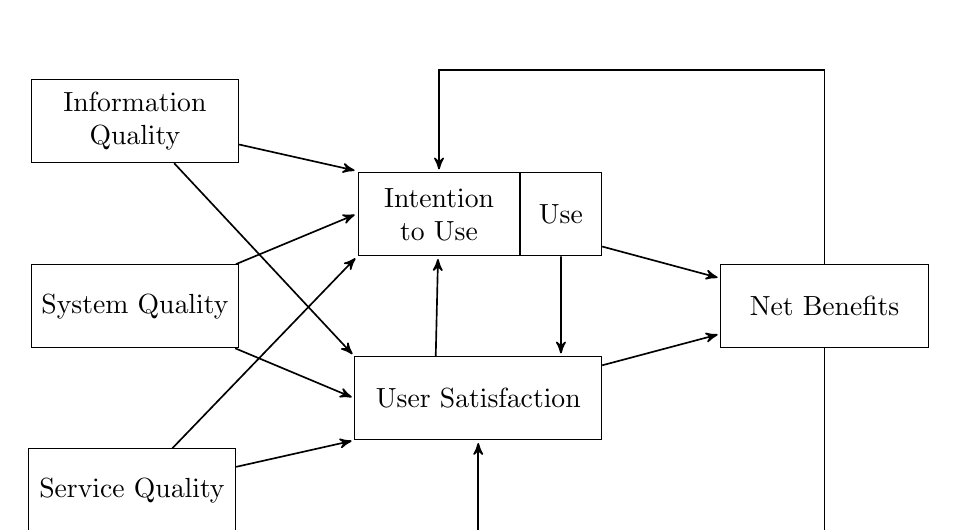
\begin{tikzpicture}
	[ node distance=1mm and 15mm,
		construct/.style={rectangle,draw,text width=2.4cm,minimum height=3em,text centered},
		arrowOut/.style={->,shorten >=1pt,>=stealth',semithick},
		arrowIn/.style={<-,shorten <=1pt,>=stealth',semithick}]
	
	\node[construct] 									(net benefits) {Net Benefits};
	
	\node[construct,text width=8mm]	(use) [above left=of net benefits] {Use};
	\node[construct,text width=18mm,node distance=1mm and 0mm] (intention) [left=of use] {Intention to Use};
	\node[rectangle,fit=(use)(intention),inner sep=0pt] (use combo) [above left=of net benefits] {}
		edge[arrowOut] (net benefits);
	
	\node[construct,text width=29mm] 	(user sat) [below left=of net benefits] {User Satisfaction}
		edge[arrowOut]	(net benefits);
		
	\node[construct] (info qual) [above left=of use combo] {Information Quality}
		edge[arrowOut] 	(use combo.north west)
		edge[arrowOut] 	(user sat.north west);
	\node[construct] (sys qual) [below left=of use combo] {System Quality}
		edge[arrowOut] 	(use combo.west)
		edge[arrowOut] 	(user sat.west);
	\node[construct] (ser qual) [below left=of user sat] {Service Quality}
		edge[arrowOut] 	(use combo.south west)
		edge[arrowOut] 	(user sat.south west);
		
	\draw[arrowOut] (net benefits) -- (0,3) -| (intention);
	\draw[arrowOut] (net benefits) -- (0,-3) -| (user sat);
	\draw[arrowOut] (use) -- ([xshift=10.5mm] user sat.north);
	\draw[arrowOut] ([xshift=-5.4mm] user sat.north) -- (intention);
\end{tikzpicture}
	\caption[Updated D\&M IS Success Model]{Updated D\&M IS Success Model \citep{DeLone2003}}
	\label{img:is_success}
\end{figure}

According to the revised model, \textit{information quality} (e.g.\ ease of understanding and completeness), \textit{system quality} (measured in metrics such as ease of use and ease of learning, usefulness, and convenience of access) and \textit{service quality} (e.g.\ reliability, responsiveness, and being up-to-date) influence \textit{user satisfaction} (e.g.\ enjoyment and overall satisfaction) and \textit{intention to use}, which is related to \textit{use} (e.g.\ amount of use and voluntariness of use), which in turn also influence each other. Use and user satisfaction also influence \textit{net benefits}, consisting of \textit{individual impact} (e.g.\ decision effectiveness, job performance), which subsequently influences \textit{organizational impact} (e.g.\ cost reductions, increased profits).

Several studies investigated the significance of the various relationships among constructs in the model. \Citet{Seddon1996} confirmed that there are significant relationships between system quality and user satisfaction, and information quality and user satisfaction. This finding means that improved information quality (which contains ease of understanding of the outputs of the system) and system quality (containing ease of use, ease of learning, and convenience of access) can lead to increased user satisfaction. Usability is a component of both of these independent variables, and thus plays a role in the relationship with user satisfaction.

\Citet{Teo1998} and \citet{Wixom2001} found that there is a significant relationship between system quality and individual impact, which means that a higher-quality system can lead to positive individual impact. Since usability is a component of system quality, it can be argued that using heuristics to increase a system's usability will lead to increased job performance and decision quality.

In addition, \citet{Teo1998} and \citet{Wixom2001} found that there is a significant relationship between information quality and individual impact (a component of \textit{net benefits} in the revised model), which means that increased understandability and usefulness of a system's output can lead to increased decision quality and job effectiveness \citep{DeLone2003}.

Overall, the model shows that usability plays an important role in information systems success, as it is a component of system quality and, to a lesser extent, of information quality and service quality. These three constructs influence user satisfaction and intention to use, which is coupled to use, and finally net benefits to the organization in which the information system is used. This network of relationships underlines the importance of good usability to ensure the success of an information system and, in continuation, the need for better tools for usability engineering.

\subsection{Task-Technology Fit}
\label{sec:ttf}
Another popular theory in this area is the task-technology fit model \citep{Goodhue1995}, in which \textit{technologies} are defined as ``tools used by individuals in carrying out their tasks'' \citep[p.\ 1828]{Goodhue1995} and \textit{tasks} are defined as ``actions carried out by individuals in turning inputs into outputs'' \citep[p.\ 1828]{Goodhue1995}. Consequently, \textit{task-technology fit} is defined as ``the extent that technology functionality matches task requirements and individual abilities'' \citep[p.\ 1829]{Goodhue1995}. This theory is relevant, since usability is an important aspect of \textit{technology characteristics}.

\begin{figure}[htb]
	\centering
	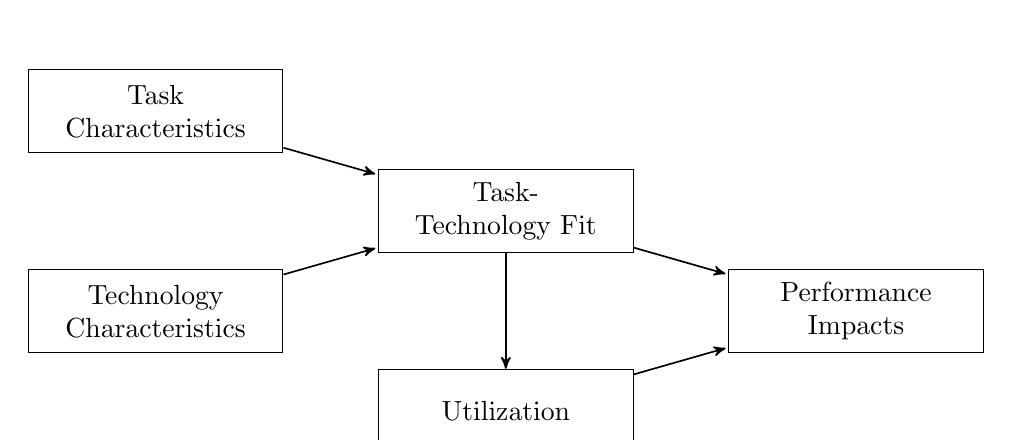
\begin{tikzpicture}
	[ node distance=2mm and 1.2cm,
		concept/.style={rectangle,draw,text width=3cm,minimum height=3em,text centered},
		arrowOut/.style={->,shorten >=1pt,>=stealth',semithick},
		arrowIn/.style={<-,>=stealth',semithick}]
		
	\node[concept] (performance) {Performance Impacts};
	\node[concept] (fit) [above left=of performance] {Task-Technology Fit}
			edge[arrowOut] 	(performance);
	\node[concept] (utilization) [below left=of performance] {Utilization}
			edge[arrowOut] 	(performance)
			edge[arrowIn] 	(fit);
	\node[concept] (task) [above left=of fit] {Task\\ Characteristics}
			edge[arrowOut] 	(fit);
	\node[concept] (technology) [below left=of fit] {Technology Characteristics}
			edge[arrowOut] 	(fit);
\end{tikzpicture}
	\caption[Task-technology fit and technology-to-performance chain]{Task-technology fit with technology-to-performance chain \citep{Goodhue1995a}}
	\label{img:ttf}
\end{figure}

\Citet{Goodhue1995a} extend the task-technology fit model with the tech\-no\-logy-to-performance chain, in order to include the influence of usage in explaining an individual's job performance. Figure~\ref{img:ttf} shows the extended task-technology fit model.

The combined model suggests that a good fit between technology, task, and the individual's characteristics, together with actual usage, will lead to improved job performance. In addition, different users are theorized to rate the same technology differently due to variances in their task needs and abilities. This means that when evaluating the usability of a system, it is important to factor in characteristics of the different tasks that users need to complete using a system, in order to ensure an actual increase in work performance \citep{Goodhue2006}.

According to the model, users will rate a technology system better if it fits the task characteristics. Since usability is an important component of a technology's characteristics, increased usability of a technology will, subject to other factors, lead to performance improvements. If the methods and tools used for usability engineering (e.g.\ heuristic evaluations) can be advanced, a technology's characteristics and fit to the task can be improved.

\section{Customer Relationship Management}
%what is it, what are crm systems
As alluded to previously, customer relationship management is the ``process of acquiring, retaining and growing profitable customers'' \citep[p.\ 8]{Brown2000}. In today's competitive marketplace, mass-advertising is often not an effective way to build lucrative relationships with customers, and thus customer relationship management becomes increasingly important in creating purposeful and tailored advertising strategies to reach customers \citep{McKenzie2001,Brown2000}. The ultimate goals of CRM are to ``win mind share, increase wallet share, and reduce churn'' \citep{McKenzie2001}.

Many companies employ computer-based systems of some form or other in an effort to realize the potential benefits of customer relationship management and to execute marketing strategies. While some systems are rudimentary, there is a large offering of specialized software for this purpose.

Most dedicated CRM systems can be grouped into one of three categories \citep{Band2010}. Enterprise CRM systems specialize in large-scale installations for companies with more than 1,000 employees, often spread across different countries. These systems are the most full-featured. Mid-market CRM systems cater to smaller companies with less than 1,000 employees and usually offer limited functionality for a cheaper price. Often, these solutions are hosted by the vendor and licensed in a software-as-a-service model. Finally, there are specialty tools, which offer a narrow band of specialized functionality, such as analytics and data management, or functionality for a specific industry such as pharmaceuticals or telecommunications \citep{Band2010}.

\subsection{Business Need, Advantages, and Problems}
%commoditization, need for tailored advertising and multiple channels Brown2000 p. 8
The business need for this type of software is increasing and driven by a commoditization of many products and a fragmentation of the marketplace and customers. This changing business environment necessitates a detailed marketing strategy with an emphasis on tailored advertising and utilization of different communication channels \citep{Brown2000}.

CRM systems support an organization in typical marketing activities by providing the functionality mentioned as follows \citep{Chaffey2011,Band2010b}.

\begin{singlespace}
	\begin{itemize}
		\item Customer selection (identify types of customers to target, segment customers)
			\begin{itemize}
				\item customer business intelligence
				\item customer data management
			\end{itemize}
		\item Customer acquisition (perform marketing activities to form relationships with new customers)
			\begin{itemize}
				\item sales force automation
				\item revenue and pricing management
				\item order management
			\end{itemize}
		\item Customer retention (perform marketing activities to maintain relationships with customers)
			\begin{itemize}
				\item electronic bill presentment and payment
				\item interactive voice response
				\item contact center infrastructure
				\item customer service and support
			\end{itemize}
		\item Customer extension (increase depth or range of products a customer purchases from the company)
			\begin{itemize}
				\item sales force automation
				\item customer service management
			\end{itemize}
	\end{itemize}
\end{singlespace}

More recently, many CRM suites have added capabilities for social media integration, support for mobile devices, and hosted software-as-a-service options. Social media integration allows CRM users to directly interact with their customers and prospects through the various social networks. Some CRM suites also allow employees within a company to network with each other and use social media-like features within the CRM system to share important information. Support for mobile devices such as smartphones and tablets is becoming increasingly important, since many salespeople want to be able to access the CRM system from their devices while on the road. Most major CRM vendors now also offer software-as-a-service solutions, which means that the vendor hosts the system and typically charges a per-use fee for access to it.

%problems with CRM (Brown2000 p. 3/4), benefits p. 8/9
There are many reasons for the adoption of CRM systems and a corresponding strategy. Costs may be reduced by employing targeted advertising models through which specific lucrative customer groups and individuals can be identified, campaigns can be tracked and assessed based on their effectiveness, and the importance of the price of a product can be reduced by providing superior customer service \citep{Brown2000}. In addition, recent research has shown that it is important to diversify marketing efforts as much as possible, since long-term customers are not necessarily more loyal than new customers, as they may still buy from a competitor who can offer better value \citep[p.\ 451]{Chaffey2011}.

\Citet{Band2010} identified the top customer relationship management goals of both business-to-business (B2B) and business-to-consumer (B2C) oriented companies. The top three benefits B2B companies seek to realize through CRM systems are attracting new customers (66\%), retaining existing customers and improving loyalty (63\%), and selling more products/services to existing customers (50\%) \citep{Band2010}. The top three CRM goals of B2C companies are retaining existing customers and improving loyalty (72\%), improving the customer experience (62\%), and attracting new customers (45\%) \citep{Band2010}.

Despite the compelling promises made about CRM systems, implementations of these systems are complex and therefore often troubled. Due to failed implementations, expected benefits are often not realized. Among the reasons for failing CRM implementations are a lack of shared understanding between different parts of the company, a lack of clear program scope, fragmented and fractional implementations, and a lack of a clear strategy for utilizing the CRM system \citep{Brown2000,McKenzie2001}.

%\subsection{Usability Issues}
%known issues with regard to usability, forrester wave
Many failed CRM system implementations have been attributed to a lack of good usability and user experience, which resulted in employee user dissatisfaction with and resistance to change toward the new system. \Citet{Kemp2001} found that a lack of alignment between users' workflow and the application's design, as well as poorly designed user interfaces, lead to many CRM implementation failures. \Citet{Ebner2003} reported usability as being a frequent source of ``trouble'' in CRM implementations. Recently though, an improvement in the usability of many CRM systems has been noted, which shows that there is an interest in resolving the problem \citet{Band2010,Band2010a}.

\subsection{Examples of CRM Software}
%examples and screen shots
\Citet{Band2010,Band2010a} identified several CRM solutions as leaders in the market for large and/or midsized companies. All of these leading solutions are either fully web-based or have at least an alternative web-based user interface. Table~\ref{tab:crm_leaders} gives an overview of these solutions. \Citet{Band2010,Band2010a} also assigned a rating for each product's usability on a scale of one through five, but it is unclear how these ratings were developed and on what they are based.

\begin{table}[hbtp]
	\vspace{0.5cm}
	\centering
	\caption[Leaders in the CRM market]{Leaders in the CRM market as identified by \citet{Band2010} and \citet{Band2010a}}
	\label{tab:crm_leaders}
	\newcolumntype{C}{>{\centering\arraybackslash}X} %
	\begin{tabularx}{\textwidth}{lCCc} \toprule
		\textbf{Solution} & \textbf{Large Companies} & \textbf{Midsize Companies} & \textbf{Usability} \\ \midrule
		Microsoft Dynamics CRM  		& \ding{51}	& \ding{51}	& 4.93 \\
		salesforce.com 				& \ding{51}	& \ding{51}	& 4.87 \\
		Oracle CRM On Demand 		& \ding{51}	& \ding{51}	& 4.54 \\
		SAP CRM 						& \ding{51}	& \ding{51}	& 4.37 \\
		Oracle Siebel CRM			& \ding{51}	& 			& 4.33 \\
		SAP Business All-in-One		&			& \ding{51}	& 4.22 \\
		CDC Software Pivotal    		& \ding{51}	& \ding{51}	& 4.13 \\
		RightNow CX 					& \ding{51}	& \ding{51}	& 3.94 \\
		SugarCRM Sugar Professional	&			& \ding{51}	& 3.90 \\
		\bottomrule
	\end{tabularx}
\end{table}

While these industry rankings and ratings are a useful tool to identify strong players and innovators, market positions can change quickly, as was recently exemplified when IBM, formerly Oracle Siebel CRM's largest customer, switched to SugarCRM, a relative new-comer and outsider due to its open source approach \citep{Jones2012}.

Section~\ref{sec:materials}\ref{sec:selected_systems} contains an overview of the three CRM systems selected as examples for the study.

\section{Usability Heuristics}
\label{sec:heuristics_review}
There are a number of different usability engineering techniques, some more expensive and complex than others. Traditional user testing, for example, calls for the inclusion of a representative sample of end users and expensive equipment to capture the user's action. Discount usability engineering techniques \citep{Nielsen1993} on the other hand are cheap, quick, and easy to perform, thus more likely to be used. Naturally, there are trade-offs that come with these benefits. First and foremost, some aspects of usability and problems may be missed when discount techniques are used. These techniques include user observation, scenarios, thinking aloud, and heuristic evaluations \citep{Nielsen1993}. It is recommended to combine these techniques to identify the largest possible number of usability problems.

User observation is an important and basic method for usability engineering in which users are asked to perform everyday tasks using an interface in their normal work environment. The researcher observes the user without interfering and takes notes about any problems the user encounters \citep{Nielsen1993}.

Scenarios use extremely simplified user interface prototypes for predefined tasks to allow users to interact with the design for a system before it is fully developed and identify usability problems. This method is very simple and allows for the review of prototypes at every iteration \citep{Nielsen1993}.

Thinking aloud is a technique in which one user at a time is asked to complete a set of tasks while ``thinking aloud'' and narrating their thought process. This method allows the researcher to gain insight into the reasoning behind a user's actions and clearly identify problematic user interface elements \citep{Nielsen1993}. It is also possible to record the user's actions on the screen as well as their commentary for further analysis.

Heuristic evaluations are a way to identify usability problems without the involvement of users. With this technique, usability experts are asked to evaluate a system based on a list of heuristics to identify usability problems that violate them \citep{Nielsen1993}. Usability problems are also often rated with regard to their severity. Many sets of heuristics have been developed for various purposes and at various levels of detail. A selection of these is presented in subsection~\ref{sec:heuristics_in_literature} below.

\subsection{Heuristics in the Literature}
\label{sec:heuristics_in_literature}
After an extensive literature review and examination of the findings, two classification schemes for usability heuristics emerged. First, heuristics can be classified by specificity, second they can be classified by granularity.

In terms of specificity, there are two broad groups---heuristics that were developed for any kind of user interface or all computer user interfaces, and heuristics focused on a particular application area such as e-commerce. Typically, the more general heuristics provide quite specific instructions and low-level guidelines for user interface design (e.g.\ icon design and layout of data entry fields). The specialized heuristics are higher-level and more concerned with workflows, task support, and industry-specific functionality (e.g.\ ability to personalize screens).

With regard to granularity, some researchers have developed specific checklists suitable for evaluating a user interface, while others only provide a set of general principles. Some research falls in between, offering intermediate granularity. As will be explained in section~\ref{sec:research_design}, the level of detail of the heuristics is relevant due to the nature of the empirical study of this thesis. Table \ref{tab:heuristics_lr} gives an overview over the heuristics research that is reviewed in this study.

\begin{table}[hbtp]
	\vspace{0.5cm}
	\centering
	\caption[Heuristics research reviewed in this study]{Heuristics research reviewed in this study; heuristics marked with a $\ast$ were used as materials for the empirical study}
	\begin{tabular}{llll} \toprule
		\textbf{Study} 					& 	& \textbf{Application Area}  & \textbf{Granularity} \\ \midrule
		\citet{Molich1990} etc. &	$\ast$ & Any kind of user interface & Principles 	\\
		\citet{Norman2002} 			& 	& Any kind of user interface & Principles 	\\
		\citet{Perlman1997}			&	& Computers									 & Principles 	\\
		\citet{Weiss1994} 			& 	& Computers 								 & Checklist		\\
		\citet{Pierotti1995} 		& 	& Computers 								 & Checklist		\\
		\citet{Leavitt2006} 		& 	& Web 											 & Checklist		\\
		%Specific heuristics
		\citet{Zhang2011}				& 	& Electronic health records	 & Principles		\\
		\citet{Petre2006} 			& 	& E-commerce 								 & Intermediate	\\
		\citet{Ardito2006}			& $\ast$	& E-learning								 & Intermediate	\\
		\citet{Oztekin2010}			& 	& E-learning								 & Intermediate	\\
		\citet{Singh2009}				& $\ast$	& ERP systems								 & Intermediate	\\
		\bottomrule
	\end{tabular}
	\label{tab:heuristics_lr}
\end{table}

\subsubsection{Classification by Granularity}
Overall, there are three distinct levels of granularity that heuristics fall into.

\paragraph{Principles} These heuristics are broadly-formulated and apply to a large number of different user interfaces and application areas. There are usually 15 or less heuristics in a set and each heuristic consists of a name and a short description. Due to the general nature of these heuristics, usability expertise is needed in order to apply them correctly and identify usability problems. They are sometimes used as the basis for developing more detailed heuristics or as categories for detailed heuristics. An example of a heuristic in this category would be ``\textit{Visibility of system status}: The system should always keep the users informed about what is going on, through appropriate feedback within reasonable time'' \citep{Nielsen1994a}.

\paragraph{Intermediate} Heuristics in this category generally apply to a specific type of user interface or application area (e.g.\ e-commerce applications) and focus on special characteristics of the application area. Since these heuristics are more detailed, there are typically between 30 and 60 items in a set. They are more specific than general principles, but less specific than checklists. An example for a heuristic in this category is ``Does the course offer multiple opportunities for interaction and communication among students, to instructor, and to content?'' \citep{Oztekin2010}.

\paragraph{Checklist} These heuristics are very detailed and low-level. They are generally used for broad application areas such as computer user interfaces in general or web user interfaces. These heuristics are most suited for a step-by-step evaluation of a user interface and often provide a rating scale for that purpose. Generally, there are more than 100 items in a set of heuristics of this type. Due to the fact that they are more detailed and specific than the other types of heuristics, they can also be used by non-usability experts to evaluate a system, but they may often seem intimidating in light of the sheer number of heuristics in a set. An example would be ``When using data entry fields, specify the desired measurement units with the field labels rather than requiring users to enter them'' \citep{Leavitt2006}.

\subsubsection{Classification by Specificity}
There are two levels of specificity with regard to application areas that heuristics can be categorized into. First, there are heuristics which are applicable to a broad spectrum of user interfaces (e.g.\ computer user interfaces in general). Second, there are heuristics which have been developed with a specific class of applications in mind (e.g.\ e-learning systems).

\paragraph{General Heuristics}
The heuristics in this section were developed for broad categories of user interfaces such as computer interfaces in general or web-based interfaces. They typically fall either into the category of principles or checklists.

%\subsection{\citeauthor{Molich1990}}
One of the earliest and best-established sets of heuristics was originally developed by \citet{Molich1990} and later refined by \citet{Nielsen1994,Nielsen1994a}. The set consists of ten general, broadly-formulated usability principles, which are applicable to most graphical user interfaces. The authors do not provide specific checklists for the evaluation of systems, but short definitions of the heuristics. Other researchers \citep[e.g.][]{Perlman1997,Lavery1996} have developed alternative descriptions and general evaluation questions for these heuristics.

%\subsection{\citeauthor{Norman2002}}
\Citet[p.\ 52]{Norman2002} identified four ``principles of good design'', \textit{visibility} [of system status], \textit{a good conceptual model}, \textit{good mappings}, and \textit{feedback}. These heuristics are general in nature and apply to not only computer user interfaces, but any kind of ``thing'' a person might interact with, be it physical or virtual. As such, these concepts are very broadly-formulated and while the author does explain them in detail, there are no concrete guidelines for a heuristic evaluation.

%\subsection{\citeauthor{Perlman1997}}
\Citet{Perlman1997} based his list of thirteen general principles on the heuristics developed by \citet{Nielsen1993} and \citet{Norman2002}. \Citeauthor{Perlman1997} took all ten of \citeauthor{Nielsen1993}'s heuristics and rephrased some of them. They were supplemented with two heuristics from \citet{Norman2002}. \Citeauthor{Perlman1997} also added two new heuristics (\textit{provide maps and a trail} and \textit{show the user what is (not) possible}). In addition, \citeauthor{Perlman1997} added short explanations for each heuristic, which differ from the existing explanations provided by the original authors of the respective heuristics.

%\subsection{\citeauthor{Weiss1994}}
\Citet{Weiss1994} developed sets of heuristics and evaluation checklists for four aspects of user interfaces (presentation, conversation, navigation, and explanation). The checklists are focused on traditional desktop-based computer systems (i.e.\ not web-based) and address both hardware and software usability. Due to the time period during which they were developed, the heuristics are mostly based on early ``green screen'' and terminal interfaces. There is a total of 285 guidelines in 20 checklists grouped into four categories. In addition to the checklists themselves, instructions for evaluating systems and selecting relevant user interface components to evaluate are provided. During an evaluation, items on the checklists are rated as fulfilled, not fulfilled, or not available. Sets of heuristics can be mixed and matched based on the specific deficiencies of the system that is to be evaluated. \Citet{Weiss1994} also provides a survey instrument for measuring user satisfaction.

%\subsection{\citeauthor{Pierotti1995}}
\Citet{Pierotti1995} created a checklist based on the items developed by \citet{Weiss1994}. The original items remained unchanged, but were regrouped into the categories identified by \citet{Nielsen1994a}. \Citeauthor{Pierotti1995} also added three new categories (\textit{skills}, \textit{pleasurable and respectful interaction with the user}, and \textit{privacy}) to accommodate all of \citeauthor{Weiss1994}'s heuristics. In addition, two new items were added to the privacy category.

%\subsection{\citeauthor{Leavitt2006}}
\Citet{Leavitt2006} provide an extensive list of 209 usability guidelines specific to web sites and web applications. The guidelines are categorized into 17 groups. The list is based on a review of the relevant literature and each item in it is rated in terms of strength of evidence and relative importance. While focused on web-based interfaces, the heuristics are still quite general in nature and not specific to the characteristics of business software.

\paragraph{Specific Heuristics}
The research in this group addresses a specific and relatively narrow field of applications or users. The heuristics are generally on a higher, less detailed level than those discussed in the previous section. These heuristics typically are of intermediate granularity, thus being neither very specific nor general.

Numerous studies have investigated heuristics for specific types of applications and systems. \Citet{Petre2006}, for example, developed a set of heuristics for e-commerce based on a list of obstacles encountered by online shoppers as they used different online stores.

E-learning has also been a popular area for the development of heuristics. \Citet{Ardito2006} developed 64 heuristics in this area. They are grouped into two broad groups: platform guidelines and module guidelines. Within these groups, there are four categories of heuristics. \Citet{Oztekin2010} developed a total of 36 heuristics in twelve categories loosely based on \citeauthor{Nielsen1994a}'s heuristics. In addition, \citet{Freire2012} provide a review of recent research on e-learning usability heuristics.

\citet{Zhang2011} developed heuristics for the area of electronic health records. These were based on the heuristics developed by \citet{Nielsen1993} as well as the ``eight golden rules'' by \citet{Shneiderman1998}. There are a total of fourteen heuristics, which are very broadly-formulated. Finally, enterprise resource planning (ERP) systems were the focus of the research by \citet{Singh2009}.

Usability heuristics have also been developed with specific types of users in mind. These include elderly users \citep[e.g.][]{AARP2004,Redish2004} and visually impaired users \citep[e.g.][]{Harper2003}.

\section{What We Know}
This section contained a review of the literature on theoretical frameworks relating to usability engineering, CRM systems, and usability heuristics. There has not been much research with regard to theoretical frameworks for usability engineering or heuristic evaluations in particular. There do exist frameworks which contain usability as a part of some of their constructs and two popular examples of these were presented.

With regard to CRM systems, we know what they are used for in organizations, who uses them, which solutions are widely used, and that implementations of CRM systems are often problematic. We do not know, which usability problems are commonly found in CRM systems and there is no set of heuristics specific to them.

Finally, there is a wealth of usability heuristics, which can be categorized according to two schemes. First, there is a spectrum of heuristics, with general heuristics on one side and domain-specific heuristics on the other. Second, there are three distinct levels of granularity, principles, checklists, and intermediate heuristics. Previous research has shown that both general and domain-specific heuristics are necessary to adequately evaluate a software system for usability problems. Yet, there are no heuristics specific to web-based CRM systems. There is also no framework for the development of specific heuristics.

\chapter{Methodology}
\label{chap:method}
This chapter contains a description of the research methodology used in this thesis. The methodology is built on existing, proven research methods, which were modified and expanded upon to answer the research question central to this thesis.

This study is guided by the following research questions:

\RQ{}

In order to identify new and obsolete usability heuristics specific to the domain of web-based customer relationship management systems, a qualitative design with three steps is employed. A collaborative group session with usability experts is held, followed by a validation through CRM users, after which the results of the two phases are analyzed and compared to existing heuristics.

First, background information about existing methods used in this study is provided. Second, the CRM systems and usability heuristics selected as input materials for the study are discussed. Third, the method for identifying eligible participants is detailed. Fourth, the research design including the structure of the group session is explained. Last, the types of data collected in this study and their sources are detailed.

\section{Background of Methods}
The protocol used for the group session is based on two existing fields of research: focus group studies and collaboration science. These areas and their applicability to this thesis are explained below.

\subsection{Collaboration Science}
The goal of the focus group session with the usability experts was to identify as many new and obsolete usability heuristics for web-based CRM software as possible. To achieve this goal, the session was structured using an approach based on collaboration science and the use of thinkLets \citep{Briggs2001}. This method has proven to build consensus more quickly, reduce session duration, and improve the quality of the end product \citep{Vreede2005}.

While the study is not a collaborative effort (in the strict sense of stakeholders working together to reach a mutually beneficial goal they can commit to), the techniques developed for collaboration science are still helpful in improving the outcome of this undertaking, because the participants are asked to work together and eventually come to a consensus about the list of heuristics for web-based CRM systems.

ThinkLets are ``the smallest unit of intellectual capital required to create one repeatable, predictable pattern of collaboration among people working toward a goal'' \citep{Briggs2003}. ThinkLets allow for the successful collaboration of groups without the need for a highly-trained facilitator by defining reusable process for collaboration in detail \citep{Vreede2005}.

In this study, a group support system (GroupSystems ThinkTank\texttrademark) is used to facilitate the session and instantiate the thinkLet patterns into a collaboration protocol. The first pattern of collaboration used in the group session is a voting activity, in which the participants vote on the heuristics presented to them. The second pattern of collaboration is a brainstorming activity, in which the participants develop ideas for new heuristics. An in-depth description of the structure of the group session is provided in section~\ref{sec:session_structure}.

%\begin{enumerate}
%	\item \textbf{Diverge}: Move from having fewer to having more concepts.
%	\item \textbf{Converge}: Move from having many concepts to a focus on and understanding of a few deemed worthy of further attention.
%	\item \textbf{Organize}: Move from less to more understanding of the relationships among concepts.
%	\item \textbf{Evaluate}: Move from less to more understanding of the benefit of concepts toward attaining a goal relative to one or more criteria.
%	\item \textbf{Build Consensus}: Move from less to more agreement among stakeholders so that they can arrive at mutually acceptable commitments.

\subsection{Focus Group Studies}
Focus group studies have an unclear background and stem from several different research fields such as marketing research, organizational research, and community development \citep[p.\ 18]{Barbour2008}. For this reason, this method has different meanings to different people and is quite flexible. Typically though, focus groups are more or less structured interviews of small groups of people led by a moderator or facilitator, who guides the participants' discussion around a specific topic \citep{Barbour2008,Morgan1998}. Focus group studies have become increasingly popular over the last two decades and are now used in research fields other than those they were used for initially \citep{Morgan1998}.

Rather than providing generalizable answers to questions, focus groups can provide insightful data about how opinions are formed and modified through group interaction as well as an in-depth understanding of the participants' opinions and perspectives \citep{Barbour2008,Edmunds1999}. Focus groups have the advantage of not putting participants ``on the spot'' if they can't answer a question \citep{Barbour2008} and the group interactions allow for the exchange of ideas and opinions between participants.

Due to the ``mixed parentage'' \citep{Barbour2008} of focus groups, many variations exist. A focus group typically consists of seven to ten participants, although ``mini focus groups'' with less participants and bigger groups with more participants have been employed as well \citep{Marshall1999,Edmunds1999}. Other variants exist, in which the focus groups sessions are performed over the phone or Internet \citep{Edmunds1999}. The participants are selected based on shared characteristics considered desirable for the study, such as expertise in a certain area \citep{Marshall1999}. The moderator should be trained and experienced in guiding and stimulating group discussions without influencing the participants.

The focus group method was chosen for the last part of the collaborative group session, wherein the participants were asked to discuss the results and their impressions of the activities completed prior to the focus group session. Table~\ref{tab:focus_group_appropriateness} shows the appropriateness of the focus group method to this study based on the strengths of the method as identified by \citet{Marshall1999}, \citet{Edmunds1999}, and \citet{Morgan1998}.

\begin{table}[hbtp]
	\centering
	\tabulinesep=_2mm^2mm
	\caption[Appropriateness of focus group method to study]{Appropriateness of the focus group method to this study \citep[wording of strengths taken from][]{Marshall1999}}
	\begin{tabu} to \textwidth {X[1,l] X[1,l]} \toprule
		\textbf{Strength of Focus Groups} & \textbf{Application to Study} \\ \midrule
		Fosters face-to-face interaction with participants & Direct interaction between participants can facilitate and accelerate consensus-building \\
		%Data collected in natural setting & \\
		Facilitates immediate follow-up for clarification & Participants can answer questions by the researcher immediately and thus improve data analysis \\
		%Good for documenting major events, crises, social conflicts & \\
		%Useful for describing complex interactions & \\
		%Facilitates discovery of nuances in culture & \\
		Provides for flexibility in formulating hypotheses & Study is exploratory and changes to the research questions are likely \\
		%Provides context information & \\
		Facilitates analysis, validity checks, and triangulation & Results of focus group activity are analyzed in conjunction with quantitative data gathered in the first two activities of the group sessions \\
		Facilitates cooperation & To achieve the ultimate goal of a single, agreed-upon list of heuristics, the participants need to cooperate and come to a consensus \\
		%Obtains large amounts of data quickly & \\
		\bottomrule
	\end{tabu}
	\label{tab:focus_group_appropriateness}
\end{table}

\Citet[p.\ 99ff]{Edmunds1999} explores the advantages and disadvantages of moderating focus groups yourself, which was the case for this study. The biggest advantages are reduced costs by forgoing the need to hire a trained professional from an outside source to moderate and analyze the focus group. In addition, a inside moderator usually also has a better understanding of the area being studied. On the other hand, an inside moderator is often biased and may impart this bias on the participants, knowingly or not. In addition, an untrained moderator can prevent the true results from emerging and thus defeats the purpose of conducting the study \citep{Edmunds1999}.

\section{Participant Selection}
Both of the two phases involved five to six participants. \Citet[p.\ 156]{Nielsen1993} recommends including five to six evaluators in a heuristic evaluation, since a group of this size is expected to find about 75\% of usability problems. Beyond this point, the number of additional problems found per evaluator decreases rapidly \citep{Nielsen1993}. For the purposes of this thesis, it is reasonable to assume that a group of participants of this size can also be expected to identify a large part of heuristics relevant to an application area, although a larger sample size may be required to increase the thoroughness. This limitation will also be discussed in section~\ref{sec:limitations}.

For the first phase, usability experts from both academia and industry were asked to participate. A minimum of three years of experience in designing and/or developing user interfaces and usability was required. Usability experts with experience in using or evaluating web-based CRM software were preferred. The second phase included actual users, who use web-based CRM software in their daily job routines. The participants were required to have at least one year of experience in working with a web-based CRM system, since they should be able to identify usability problems and other characteristics of this type of software that may affect the development of heuristics.

Usability experts were recruited through personal contacts. CRM users were recruited through personal contacts as well as snowball sampling, in which the recruited usability experts were asked to identify and invite CRM users in their organization.

\section{Research Design}
\label{sec:research_design}

\begin{figure}[htbp]
	\centering
	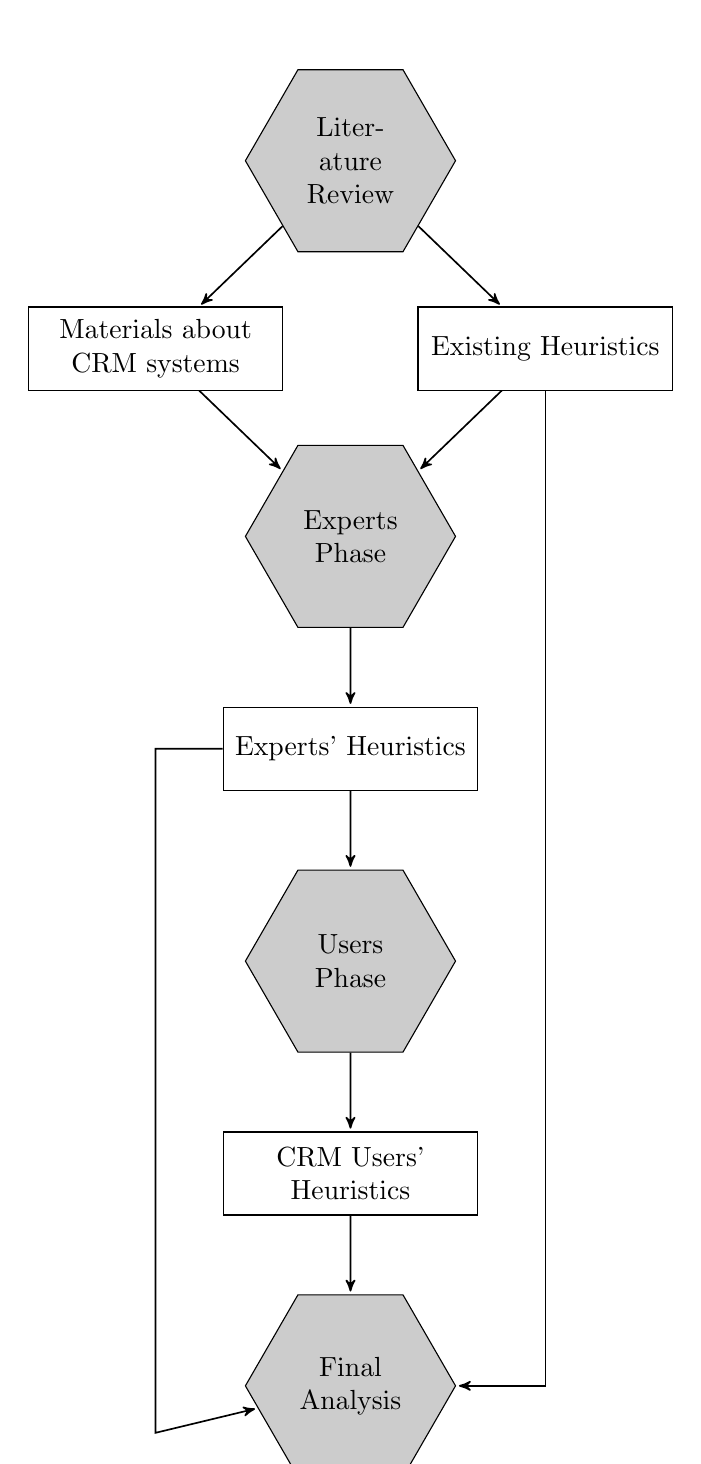
\begin{tikzpicture}
	[ node distance=10mm and 0mm,
		activity/.style={regular polygon,regular polygon sides=6,draw,fill=black!20,text width=1.4cm,text centered},
		document/.style={rectangle,draw,text width=3cm,minimum height=3em,text centered},
		arrowOut/.style={->,shorten >=1pt,>=stealth',semithick},
		arrowIn/.style={<-,shorten <=1pt,>=stealth',semithick}]
			
	\node[document] (materials) {Materials about CRM systems};
	\node[activity] (literature) [above right=of materials] {Lit\-er\-a\-ture Review};
	\node[document] (existing heuristics) [below right=of literature] {Existing Heuristics};
	\node[activity] (group one) [below right=of materials] {Experts Phase};
	\node[document] (expert heuristics) [below=of group one] {Experts' Heuristics};
	\node[activity] (group two) [below=of expert heuristics] {Users Phase};
	\node[document] (user heuristics) [below=of group two] {CRM Users' Heuristics};
	\node[activity] (analysis) [below=of user heuristics] {Final Analysis};
	
	\draw[arrowOut] (literature) -- (materials);
	\draw[arrowOut] (literature) -- (existing heuristics);
	\draw[arrowOut] (materials) -- (group one);
	\draw[arrowOut] (existing heuristics) -- (group one);
	\draw[arrowOut] (existing heuristics) |- (analysis);
	\draw[arrowOut] (group one) -- (expert heuristics);
	\draw[arrowOut] (expert heuristics) -- (group two);
	\draw[arrowOut] (expert heuristics) -| (0,-13.77) -- (analysis);
	\draw[arrowOut] (group two) -- (user heuristics);
	\draw[arrowOut] (user heuristics) -- (analysis);
\end{tikzpicture}
	\caption{Research design}
	\label{img:research_design}
\end{figure}

Figure~\ref{img:research_design} provides an overview of the research design, which consists of four activities based on the development of three sets of heuristics. First, a literature review was conducted. During the literature review, important and relevant usability heuristics were researched and collected. These heuristics served as the basis for the subsequent steps and were eventually used in the final analysis.

Second, a focus group session with usability experts was used to identify heuristics specific to web-based CRM systems. The experts used their judgement to select still-relevant heuristics from the lists identified as part of the literature review, and supplemented them with new heuristics as suitable to cover the characteristics of web-based CRM software.

Third, a validation phase with actual users of a web-based CRM system was completed. This step aimed to increase the internal validity of the results by including the perspectives of users. The participants in this step were given the list of heuristics created in the first phase and were asked to rate the heuristics based on their perceived applicability. After the rating, the participants were asked to identify missing heuristics.

Fourth, the results of the two phases were analyzed to identify the points on which the usability experts and the CRM users agree and on which they disagree. The resulting set of proposed heuristics for web-based CRM systems was then compared to the heuristics used as the initial input for the first focus group. In comparing this new set of heuristics to existing heuristics identified in the literature review, it can then be determined which heuristics have become irrelevant for this class of software, and which new ones need to be added to heuristic evaluations in order to reduce the likelihood of missing problems and to cover as much of the system to be evaluated as possible.

An important consideration is the level of detail at which heuristics are to be evaluated. Some existing sets are high-level and only provide few principles \citep[e.g.][]{Molich1990}, others are detailed and consist of hundreds of items \citep[e.g.][]{Leavitt2006}. For this study, a middle ground was sought by aiming for around fifty to sixty items in the final list. The items were intended to be more specific than stating a general principle like ``consistency'', but less specific than, for example, stating that ``each save button is in the same location''. A heuristic at the right level might be ``buttons are always in the same location''.

\subsection{Pilot}
A pilot study was conducted to help ensure the actual focus group sessions will run smoothly. The goal of the trial run was to uncover potential weaknesses or problems with the procedures so they could be rectified before the actual sessions. The data resulting from the trial run were not used for this study, as the trial's purpose was only to test procedures.

A group of fourteen undergraduate students participated in the trial run. The trial run was performed as a part of the final exam for a user interface design course at the University of Nebraska at Omaha.

For this reason, a number of modifications to the protocol used in the actual sessions had to be made. First, due to the limited amount of time available for the pilot, the students were asked to evaluate only one specific system instead of a class of systems. In addition, an abbreviated list of 26 heuristics was used as the basis for the evaluation. Second, the students were not sufficiently trained to develop new heuristics for the system, so they were only asked to evaluate existing heuristics given to them with regard to applicability. Third, the students were also asked to identify usability problems based on the heuristics supplied to them to satisfy the requirements for the final exam of the class they were taking.

The students were asked to evaluate a student information system familiar to them on the basis of heuristics supplied to them \citep[a modified version of the set developed by][see appendix~\ref{app:trial}]{Oztekin2010}. The students also received a short list of usage scenarios to aid them in purposefully interacting with the system (also in appendix~\ref{app:trial}). Since some of the heuristics were not directly applicable to the system in question, the students were also asked to state whether they believe the heuristics to be appropriate.

After the evaluation phase, the students were asked to discuss the identified usability problems to create a unified list. They were asked to name the usability problems they saw most often in the list they created during the previous activity. The moderator then inserted the problems every student agreed on into a single list in preparation for the final activity. As a last step, the participants rated the usability problems in the list by severity on a three-point scale of ``high'', ``medium'', and ``low''.

During the trial run, no significant problems with the protocol were encountered. The participants were able to understand the instructions and use the group support system easily. Overall, the students also understood the heuristics and were able to evaluate them with regard to their applicability to the student information system used for this pilot.
%results? What type of comments did you get?

The duration of the trial run was limited to one hour, because it was only a part of a exam. This amount of time was far too short to complete the entire protocol. Only 26 heuristics were used and it took most students 45 minutes to comment on each of them. A time frame of one hour for the evaluation component should have provided sufficient time. The subsequent discussion was ended after 15 minutes due to the time constraints mentioned previously. A longer period would have allowed for a more complete discussion. In consequence, a period of three hours was estimated to be necessary to complete the full protocol with the two focus groups.

\section{Research Study}
\subsection{Pre-Tasking}
In preparation for the study, the usability experts were asked to review pre-task material. This is an important step for increasing the level of detail the participants were able to produce, as well as getting them in the right mindset by providing context \citep[p.\ 164]{Cooper2011}.

In order for the participants of the first phase to be able to prepare, the list of existing heuristics from the literature review was provided to them prior to the session for their review. The participants were asked to examine the existing heuristics and start thinking about whether they might be relevant to web-based CRM systems. In addition, screen shots of exemplary systems were sent to the participants to provide visual context and stimuli for developing new heuristics specific to the class of systems at hand.

\subsection{Materials}
\label{sec:materials}
\subsubsection{CRM Systems}
\label{sec:selected_systems}
Based on their leading role in the markets for both large and midsized companies, as well as their wide adoption and availability of documentation, Microsoft Dynamics CRM and salesforce.com were selected as examples of web-based CRM software for this thesis' focus group sessions, which are explained in detail in chapter~\ref{chap:method}. In addition, SugarCRM Sugar Professional was selected, even though it is less present in the enterprise market, because it has the lowest usability rating of the nine leaders and is the only open-source product among them.

\paragraph{Microsoft Dynamics CRM}
Microsoft Dynamics CRM claims to power business productivity through its cloud-based offering. The product can be accessed through a web browser or through a Microsoft Outlook add-in. The software is similar to many of the other Microsoft products in terms of functionality and usability, which makes it familiar to many users \citep{Band2010}. Microsoft Dynamics CRM has the second-strongest presence in the market for enterprise CRM systems, ranking right after Oracle Siebel CRM \citep{Band2010}. Example screen shots of the system are available in appendix section~\ref{appsec:microsoft}.

\paragraph{salesforce.com}
Transforming companies into ``social enterprises'' is the goal of salesforce.com, which they aim to achieve through a strong focus on social media integration and enabling of organization-internal collaboration. The solution is fully web-based and available in a subscription-based software-as-a-service (SaaS) pricing and delivery model, which makes it attractive for organizations not wanting to spend time and money creating an on-premises infrastructure for this purpose. Salesforce.com has the fourth-largest presence in the market for enterprise CRM solutions \citep{Band2010}, and is actually the leader in terms of market presence for midsized companies \citep{Band2010a}. Example screen shots are available in appendix section~\ref{appsec:salesforce}.

\paragraph{SugarCRM Sugar Professional}
As the largest open-source system in the market, SugarCRM is in a special position, since it offers a free edition of its product. Besides the free edition, there are various paid editions with differing levels of service. Paid editions are also available in a hosted delivery model, but all versions can be installed on premises. Due to the open-source status, there is an active developer and support community. Example screen shots are available in appendix section~\ref{appsec:sugarcrm}.

\subsubsection{Usability Heuristics}
The ten heuristics developed by \citet[p.\ 30]{Nielsen1994a} were selected as the basis for the materials for the empirical study, since they are established and well-known general principles.

Two medium-grain sets of heuristics were selected to investigate whether these are considered more or less applicable to the class of systems targeted by this study. One of them was developed for ERP systems, which is a class of systems fairly similar to CRM systems; the other was developed for e-learning systems, which have a quite different set of users and purpose.

The heuristics by \citet{Ardito2006} were chosen to represent the heuristics for systems dissimilar to CRM systems. Finally, the heuristics by \citet{Singh2009} were selected, because ERP systems are similar to CRM systems in terms of users and purpose.

No heuristics at the checklist level were included, because there are too many per set and they are not application-specific. \Citeauthor{Nielsen1994a}'s heuristics were included to represent the general heuristics instead.

\subsection{Session Structure}
\label{sec:session_structure}
The two phases followed two similar structures. Both sessions involved five to six participants and consisted of a quantitative rating activity followed by a qualitative discussion activity.

The differences lie in the input materials, the nature of the qualitative activity, as well as the participants. For the usability expert session, the background materials included a list of existing usability heuristics identified in the literature review. For the CRM user session on the other hand, the materials consisted only of the list of heuristics created by the usability experts in the first session.

Another difference is that the first phase was based on a focus group session, during which all participants collaborated. During the second phase, the participants did not collaborate, but completed the rating and discussion activities individually through an online questionnaire and a phone interview with the researcher respectively.

Figure~\ref{img:session_structure_experts} shows the structure of the usability expert session and figure~\ref{img:session_structure_users} shows the structure of the CRM user session.

\begin{figure}[htbp]
	\centering
	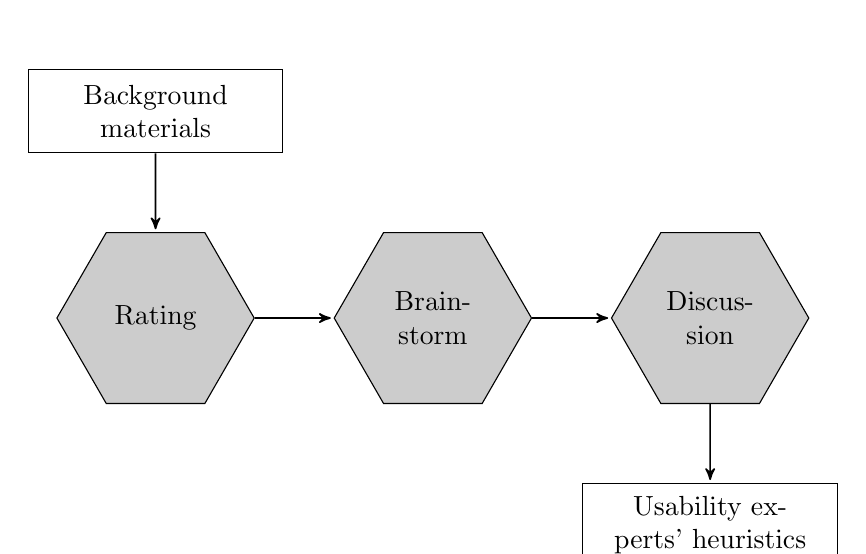
\begin{tikzpicture}
[ node distance=10mm and 10mm,
		activity/.style={regular polygon,regular polygon sides=6,draw,fill=black!20,text width=1.3cm,text centered},
		document/.style={rectangle,draw,text width=3cm,minimum height=3em,text centered},
		arrowOut/.style={->,shorten >=1pt,>=stealth',semithick},
		arrowIn/.style={<-,shorten <=1pt,>=stealth',semithick}]
			
	\node[document] (materials) {Background materials};
	\node[activity] (voting) [below=of materials] {Rating};
	\node[activity] (brainstorming) [right=of voting] {Brain\-storm};
	\node[activity] (discussion) [right=of brainstorming] {Discus\-sion};
	\node[document] (final list) [below=of discussion] {Usability experts' heuristics};
	
	\draw[arrowOut] (materials) -- (voting);
	\draw[arrowOut] (voting) -- (brainstorming);
	\draw[arrowOut] (brainstorming) -- (discussion);
	\draw[arrowOut] (discussion) -- (final list);
\end{tikzpicture}
	\caption{Structure of the collaborative session with usability experts}
	\label{img:session_structure_experts}
\end{figure}

\begin{figure}[htbp]
	\centering
	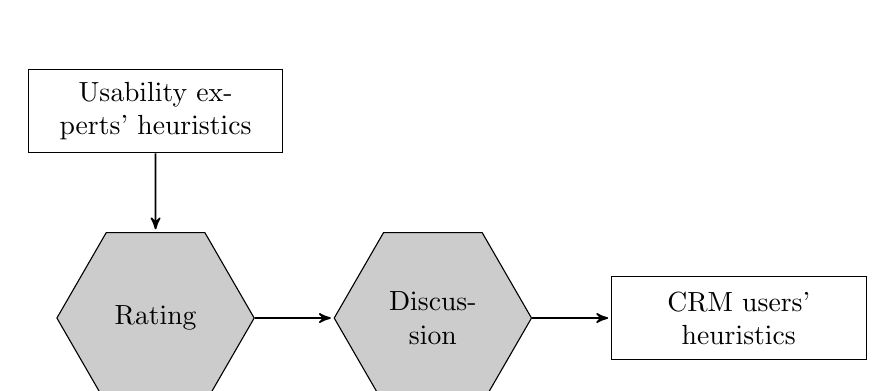
\begin{tikzpicture}
[ node distance=10mm and 10mm,
		activity/.style={regular polygon,regular polygon sides=6,draw,fill=black!20,text width=1.3cm,text centered},
		document/.style={rectangle,draw,text width=3cm,minimum height=3em,text centered},
		arrowOut/.style={->,shorten >=1pt,>=stealth',semithick},
		arrowIn/.style={<-,shorten <=1pt,>=stealth',semithick}]
	
	\node[document] (first list) {Usability experts' heuristics};	
	\node[activity] (second rating) [below=of first list] {Rating};
	\node[activity] (second discussion) [right=of second rating] {Discus\-sion};
	\node[document] (second heuristics) [right=of second discussion] {CRM users' heuristics};
	
	\draw[arrowOut] (first list) -- (second rating);
	\draw[arrowOut] (second rating) -- (second discussion);
	\draw[arrowOut] (second discussion) -- (second heuristics);
\end{tikzpicture}
	\caption{Structure of the validation phase with CRM users}
	\label{img:session_structure_users}
\end{figure}

\subsubsection{First Phase: Usability Experts}
First, the participants were asked to review the list of heuristics provided to them in the group support system (see appendix~\ref{app:first_group}) and to assign two ratings to each heuristic. The first rating allowed the participants to specify how applicable each of the provided heuristics is to web-based CRM systems in their opinion. This rating was assigned on a five-point numeric scale. The second rating allowed the participants to indicate whether they think any modifications were necessary in order to make a heuristic more applicable (e.g.\ whether wording needed to be changed).

After the first activity, a brainstorming session followed. The participants were asked to re-evaluate the heuristics which received the highest rating for ``need for rewording'' in the previous phase. The participants reworded heuristics were possible and discarded the others. Finally, the participants discussed any ideas for heuristics they thought needed to be added to account for web-based CRM systems as extensively as possible. The group support system also allowed for participants to interact and comment on each others' ideas in addition to the verbal discussion.

\subsubsection{Second Phase: CRM Users}
First, the participants of this phase were asked to review the list of heuristics developed by the usability experts and assign a rating to each. This rating allowed the participants to specify how applicable they think each heuristic is to web-based CRM systems. The rating was assigned on a five-point numeric scale with an additional option of ``don't know'' for cases in which a participant may not understand a heuristic. The questionnaire with the heuristics was made available to the participants in a web-based survey tool.

The researcher then called each participant to administer a follow-up interview. In order to refresh the participants' memory of the usability heuristics, the first questions were ``What do you like about your CRM system?'' and ``What don't you like about your CRM system?''. The participants were then asked to give their overall impression of the applicability of the heuristics they saw in the questionnaire and to identify any areas they felt were not addressed properly by the heuristics. Finally, the participants were asked about the heuristics which were added by the usability experts in order to place a special emphasis on validating their legitimacy.

This phase was conducted with individual interviews as opposed to the focus group approach utilized in the first phase. The main reason for this difference was that the participants in the second phase were less willing to make the bigger time commitment required by the group set-up. \Citet{Robinson1993} found that there is no significant difference in the number and quality of responses obtained through group versus individual interviews. Therefore the change in protocol was not felt to be a problem in answering the research question.

\section{Data Sources and Analysis}
During the study, both quantitative and qualitative data were collected. Quantitative data was collected during the first activity of the two phases, wherein the participants' votes on the applicability of the presented usability heuristics were collected. For the group session, this means data about the participants' opinions of the applicability of existing usability heuristics to the specific context of web-based CRM systems. For the second phase, the votes captured the participants' agreement with the results from the first group session, as the participants' votes indicate their opinions of the applicability of the heuristics developed in the first group session to web-based CRM systems.

Qualitative data was collected during the later activities of each phase. During these activities, the participants provided comments and opinions about the usability heuristics presented to them. During the first phase, the participants engaged in a group discussion about the reviewed heuristics, their need for rewording, as well as any areas missing from the heuristics. During the second phase, the participants engaged in one-on-one phone interviews with the researcher to discuss their overall impression of the heuristics, any missing areas, as well as a targeted discussion of the heuristics newly added by the usability experts.

\subsection{Analysis of Quantitative Data}
Due to the small number of participants in the study, the options for statistical analysis of the data are limited. For the quantitative data collected in the rating activity, descriptive statistics such as means and variance were used to determine overall scores for each heuristic. The heuristics were then sorted based on their applicability score and divided into two groups. The analysis performed on the data is available in sections~\ref{sec:evaluation_existing_first} and~\ref{sec:evaluation_existing_second}.

\subsection{Analysis of Qualitative Data}
Focus group analysis can be challenging and deserves special attention. It is important to note that focus group analysis already starts during the session itself. \Citet{Krueger1998} recommends a systematic approach to focus group analysis consisting of six steps, which were followed while analyzing the data in this study. First, the questions for the participants should be ordered in a way that maximizes insight by allowing for enough time for the participants to order their thoughts and exchange opinions with the other participants. Only then should the actual topical questions be asked. During the focus group, comments should be electronically recorded. In addition, notes should be taken by an assistant moderator, since the main moderator is not likely to have enough time to take thorough notes. At the end of the focus group, it is important to get participant verification, by letting every participant summarize their main points or reading the moderators' notes to the participants and ensuring they agree to them.

Immediately after the focus group, the moderator and other participating personnel should debrief and talk about any important points or quotes they remember. This debriefing should also be recorded electronically for later reference. During the main analysis process, labels should be attached to main ideas or phenomena. These labels or codes are then used as the basis for further analysis such as identifying counts of codes and combinations in which they occur. The final step recommended by \citet{Krueger1998} comes after the analysis: preliminary and final reports should be shared with participants and stakeholders.

\chapter{Results}
\label{chap:findings}
This chapter presents the results of this thesis based on the two parts of the study. First, the results of the session with usability experts are presented. Second, the results of the session with CRM users are presented. Both of these sections consist of a description of the participants and an overview and analysis of the outcomes. Finally, a comparative analysis is conducted to investigate the commonalities and differences between the results of the first and second phases. Finally, a unified list of usability heuristics for web-based CRM systems is created.

\section{Phase One}
The first session was administered on June 28th, 2012, and took 2.5 hours. During the first segment, which lasted approximately one hour, participants were briefed and then rated existing heuristics presented to them in the group support system. After a break, the participants engaged in a group discussion during which they were asked to reword those heuristics which were identified to be in need of rewording to be more applicable to web-based CRM systems. Finally, the participants were asked to develop new heuristics specific to web-based CRM systems in a group discussion. The two discussions in the second part of the session took one hour.

\subsection{Participants}
Five usability experts participated in the first session. Table~\ref{tab:first_participants} gives an overview of the participants' experience relevant to this study. All participants had at least four years of experience evaluating, designing, or developing user interfaces, and at least 2.5 years of professional experience in the usability field. Although one participant only had 2.5 years of professional experience in the usability field, he completed a Master's degree in human-computer interaction and had research experience in the field. The mean number of years of professional experience was 9.7, while the mean number of years evaluating, designing, or developing user interfaces was 11.4.

The participants' experience with CRM systems was much less extensive. Two out of the five participants had no experience using a CRM system, with the mean being 1.2 years of experience. Only two people had any experience evaluating, designing, or developing CRM systems (three years and 0.1 years of experience respectively).

\begin{table}[hbtp]
	\centering
	\vspace{0.5cm}
	\caption{Years of experience with usability and CRM systems of the participants of the first session}
	\begin{tabular}{lrrrrr} \toprule
		& \multicolumn{5}{c}{\textbf{Participant}} \\
		\textbf{Years of Experience\ldots{}} & \textbf{A} & \textbf{B} & \textbf{C} & \textbf{D} & \textbf{E} \\ \midrule
		working in the usability field 							& 6 & 10 & 15 & 15 & 2.5 \\
		evaluating, designing, or developing user interfaces	& 6 & 17 & 15 & 15 & 4 \\
		using a CRM system										& 0 &  3 &  1 &  2 & 0 \\
		evaluating, designing, or developing CRM systems		& 0 &  3 &  0 &  0 & 0.1 \\
		\bottomrule
	\end{tabular}
	\label{tab:first_participants}
\end{table}

\subsection{Evaluation of Existing Heuristics}
\label{sec:evaluation_existing_first}
The first activity of the session consisted of a rating of the existing heuristics based on their applicability to web-based CRM systems and their need for rewording to become more applicable. The ratings for applicability were performed on a five-point scale ranging from ``not applicable'' (1) to ``highly applicable'' (5). The ratings for the need for rewording were performed on a dichotomous scale (``no'' (0) and ``yes'' (1)). Responses to all heuristics on both scales were mandatory.

In total, 84 existing heuristics were used during the first activity of the first session. Ten were taken from \citet{Nielsen1994a}, 35 from \citet{Singh2009}, and 39 from \citet{Ardito2006}. Table~\ref{tab:first_results_bysource} shows selected descriptive statistics for the heuristics based on their source. Overall, the general heuristics developed by \citet{Nielsen1994a} etc.\ were rated as the most applicable with the least need for rewording. The heuristics specific to ERP systems developed by \citet{Singh2009} were rated as slightly less applicable than the first set, with a higher need for rephrasing. Finally, the e-learning heuristics developed by \citet{Ardito2006} received the lowest overall scores with regard to applicability and the highest scores with regard to their need for rewording.

\begin{table}[htbp]
	\centering
	\vspace{0.5cm}
	\caption[Overall applicability and need for rewording by heuristics source]{Overall applicability and need for rewording by heuristics source; \textit{applicability} was measured on a five-point scale (1-5), \textit{need for rewording} was measured on a binary scale (0, 1)}
	\label{tab:first_results_bysource}
	\begin{tabular}{lrrrrrr} \toprule
			& \multicolumn3{c}{\textbf{Applicability}} & \multicolumn3{c}{\textbf{Need for Rewording}} \\
			\textbf{Source} & \textbf{Mean} & \textbf{Min.} & \textbf{Max.} & \textbf{Mean} & \textbf{Min.} & \textbf{Max.} \\ \midrule
		\citet{Nielsen1994a}	& 4.100 & 3.8 & 4.6 & 0.040 & 0.0 & 0.4 \\
		\citet{Singh2009}		& 3.709 & 1.4 & 4.6 & 0.246 & 0.0 & 0.8 \\
		\citet{Ardito2006}		& 2.708 & 1.4 & 4.6 & 0.303 & 0.0 & 0.8 \\
		\bottomrule
	\end{tabular}
\end{table}

Figure~\ref{img:first_cumulative} provides an overview of the number of heuristics with a given rating of applicability as well as a cumulative count of heuristics based on their applicability rating. There is no clear natural grouping of heuristics (i.e.\ a clear cut-off or separation between highly applicable heuristics and less applicable heuristics), but there are two somewhat distinct groups (heuristics rated 2.6 or below and heuristics rated 3 and above). The lower group comprises 21 heuristics (25\%), the upper group 56 heuristics (66.67\%). Seven heuristics (8.33\%) received a rating of 2.8, which lies between these groups.

\begin{figure}[htbp]
	\centering
	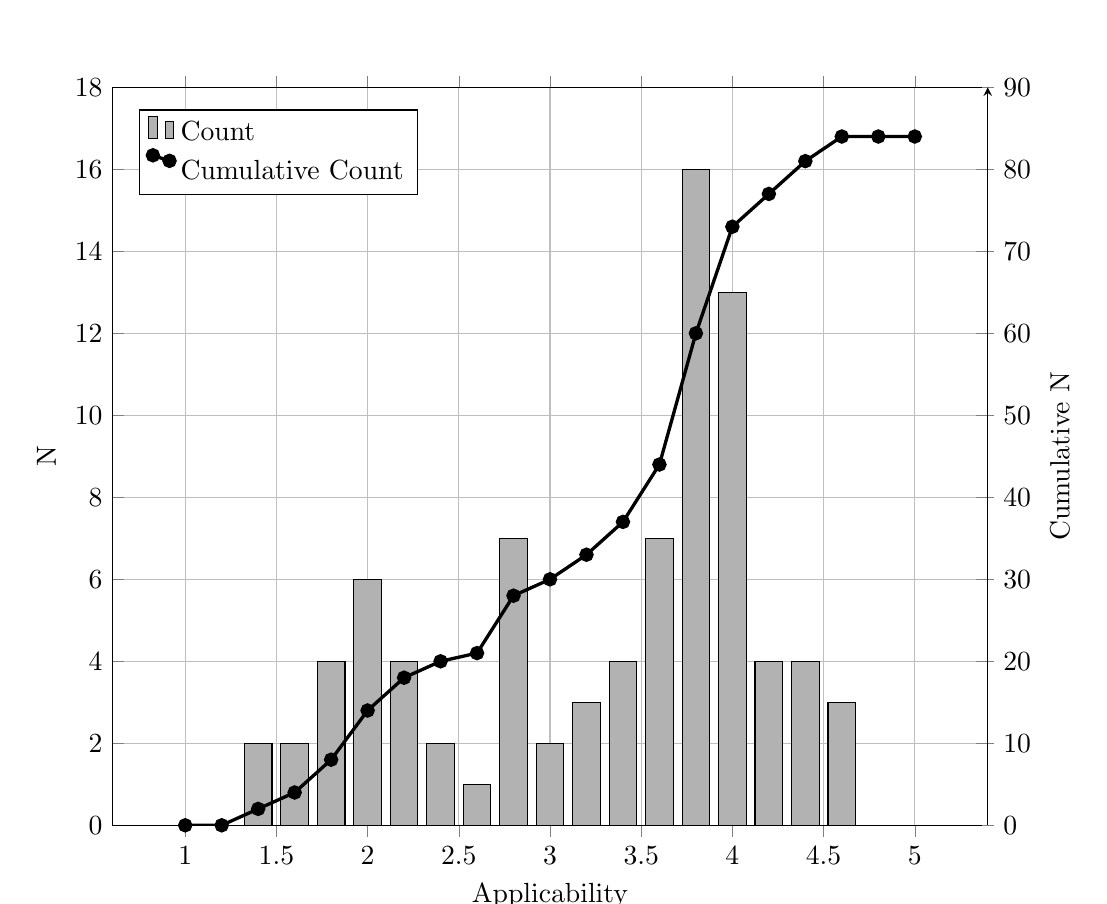
\begin{tikzpicture}
	\begin{axis} [
		xlabel=Applicability,
		ylabel=N,
		grid=major,
		legend pos=north west,
		legend cell align=left,
		ybar,
		ymin=0,
		ymax=18
	]
		\addplot[fill=black!30] coordinates {
			(1.0, 0) (1.2, 0) (1.4, 2) (1.6, 2) (1.8, 4) (2.0, 6) (2.2, 4) (2.4, 2) (2.6, 1) (2.8, 7) (3.0, 2) (3.2, 3) (3.4, 4) (3.6, 7) (3.8,16) (4.0,13) (4.2, 4) (4.4, 4) (4.6, 3) (4.8, 0) (5.0, 0)
		};
		\addlegendentry{Count}
		\addlegendimage{sharp plot,mark=*,very thick}
		\addlegendentry{Cumulative Count}
	\end{axis}
	
	\begin{axis} [
		ylabel=Cumulative N,
		axis y line=right,
		axis x line=none,
		ybar,
		ymin=0,
		ymax=90
	]
		\addplot[sharp plot,mark=*,very thick] coordinates {
			(1.0,0) (1.2,0) (1.4,2) (1.6,4) (1.8,8) (2.0,14) (2.2,18) (2.4,20) (2.6,21) (2.8,28) (3.0,30) (3.2,33) (3.4,37) (3.6,44) (3.8,60) (4.0,73) (4.2,77) (4.4,81) (4.6,84) (4.8,84) (5.0,84)
		};
	\end{axis}
\end{tikzpicture}
	\caption{Count and cumulative count of heuristics based on applicability rating by usability experts}
	\label{img:first_cumulative}
\end{figure}

Figure ~\ref{img:first_by_source} shows the percentage of heuristics achieving a given applicability rating by source. Clearly, \citeauthor{Nielsen1994a}'s heuristics performed well, as they all achieved a rating of 3.8 or more. The ratings for the heuristics developed by \citet{Singh2009} are more dispersed, but with the exception of one outlier, achieved ratings of 2.8 or more. The e-learning heuristics developed by \citet{Ardito2006} were rated least applicable to web-based CRM systems on average, but were also the most dispersed.

\begin{figure}[htbp]
	\centering
	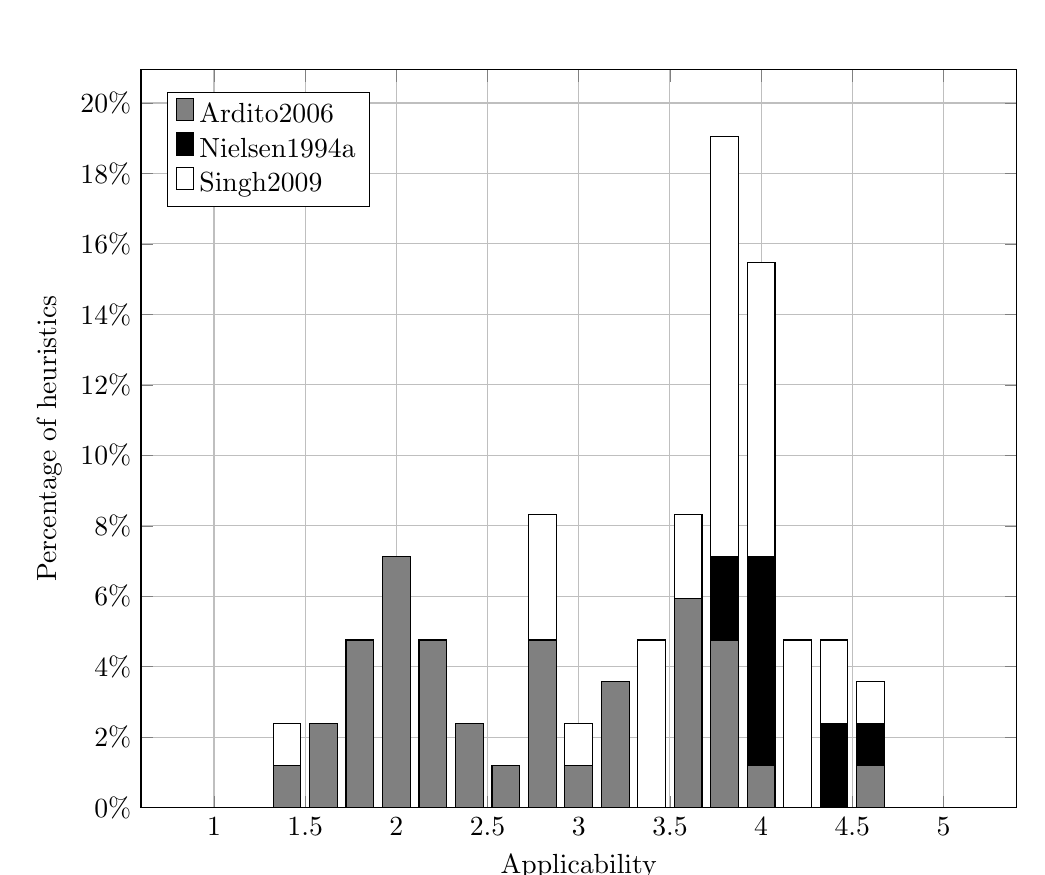
\begin{tikzpicture}
	\begin{axis} [
		xlabel=Applicability,
		ylabel=Percentage of heuristics,
		grid=major,
		legend pos=north west,
		legend cell align=left,
		ybar stacked,
		ymin=0,
		yticklabel=\pgfmathprintnumber{\tick}\%
	]
		\addplot[fill=black!50] coordinates {
			(1.00,0.00) (1.20,0.00) (1.40,1.19) (1.60,2.38) (1.80,4.76) (2.00,7.14) (2.20,4.76) (2.40,2.38) (2.60,1.19) (2.80,4.76) (3.00,1.19) (3.20,3.57) (3.40,0.00) (3.60,5.95) (3.80,4.76) (4.00,1.19) (4.20,0.00) (4.40,0.00) (4.60,1.19) (4.80,0.00) (5.00,0.00) 
		};
		\addlegendentry{\citet{Ardito2006}}
		
		\addplot[fill=black] coordinates {
			(1.00,0.00) (1.20,0.00) (1.40,0.00) (1.60,0.00) (1.80,0.00) (2.00,0.00) (2.20,0.00) (2.40,0.00) (2.60,0.00) (2.80,0.00) (3.00,0.00) (3.20,0.00) (3.40,0.00) (3.60,0.00) (3.80,2.38) (4.00,5.95) (4.20,0.00) (4.40,2.38) (4.60,1.19) (4.80,0.00) (5.00,0.00)
		};
		\addlegendentry{\citet{Nielsen1994a}}
		
		\addplot[fill=white] coordinates {
			(1.00,0.00) (1.20,0.00) (1.40,1.19) (1.60,0.00) (1.80,0.00) (2.00,0.00) (2.20,0.00) (2.40,0.00) (2.60,0.00) (2.80,3.57) (3.00,1.19) (3.20,0.00) (3.40,4.76) (3.60,2.38) (3.80,11.90) (4.00,8.33) (4.20,4.76) (4.40,2.38) (4.60,1.19) (4.80,0.00) (5.00,0.00)
		};
		\addlegendentry{\citet{Singh2009}}
	\end{axis}
\end{tikzpicture}
	\caption{Percent of all heuristics with a given rating of applicability by source}
	\label{img:first_by_source}
\end{figure}

If an applicability rating of 3 is chosen as a cut-off for selecting heuristics deemed applicable to web-based CRM systems, a total of 56 heuristics are included and 28 excluded. Of the included heuristics, 15 were developed by \citet{Ardito2006}, 10 were developed by \citet{Nielsen1994a}, and 31 were developed by \citet{Singh2009}. Table~\ref{tab:first_results_cut-off} shows the number of heuristics included from each source given an applicability rating cut-off of 3.

\begin{table}[htbp]
	\centering
	\vspace{0.5cm}
	\caption{Heuristics above and below cut-off by source}
	\label{tab:first_results_cut-off}
	\begin{tabular}{lrrrr}	\toprule
		\textbf{Source} & $\mathbf{N}$ & $\mathbf{N \boldsymbol{\geq} 3}$ & $\mathbf{N \boldsymbol{<} 3}$ & $\mathbf{\boldsymbol{\%} N \boldsymbol{\geq} 3}$ \\ \midrule
		\citet{Ardito2006} 		& 39 & 15 & 24 	&  38.64 \\
		\citet{Nielsen1994a} 	& 10 & 10 & 0 	& 100.00 \\
		\citet{Singh2009} 		& 35 & 31 & 4 	&  88.57 \\ \midrule
		Total					& 84 & 56 & 28 	&  66.67 \\
		\bottomrule
	\end{tabular}
\end{table}

A detailed table with the mean and standard deviation for each heuristic's applicability to CRM systems and need for rewording is available in appendix section~\ref{appsec:results_first}.

\FloatBarrier
\subsection{Development of New Heuristics}
The first step in developing new heuristics for web-based CRM systems was an evaluation of the heuristics with a rated need for rewording of 0.5 or more (i.e.\ more than half of the participants indicated that the heuristic needed to be reworded). All heuristics with a rating for ``need for rewording'' of 0.5 or greater were included in this activity, regardless of their applicability rating. There were a total of 13 heuristics in this category. Of the 13 heuristics, only four received a rating of applicability of three or greater. Heuristics with a low applicability rating were included, because it was anticipated their applicability could be improved through rewording.

None of the heuristics developed by \citet{Nielsen1994a} received a rating of 0.5 or greater, but six of the heuristics developed by \citet{Singh2009} and seven of the heuristics developed by \citet{Ardito2006} were in need of rewording.

The participants engaged in a group discussion focused on identifying specific problems with the heuristics in need of rewording, and establishing alternative heuristics on their basis. During the discussion, the participants identified different themes of problems with the heuristics. Table~\ref{tab:first_results_rewording_themes} gives an overview over these themes and how often they occurred. Some heuristics were associated with more than one theme.

\begin{table}[htbp]
	\centering
	\vspace{0.5cm}
	\caption[Problems identified with heuristics in need of rewording]{Problems identified with heuristics in need of rewording; A = number of heuristics per problem theme developed by \citet{Ardito2006}, S = number of heuristics per problem theme developed by \citet{Singh2009}}
	\label{tab:first_results_rewording_themes}
	\begin{tabular}{lrrrr}	\toprule
		\textbf{Problem Theme} 	& \textbf{A} & \textbf{S} & \textbf{Total} & \textbf{Reworded} \\ \midrule
		Difficult to understand & 4 & 2 & 6 & 3 \\
		Domain-specific wording & 5 & 0 & 5 & 3 \\
		Too vague and general 	& 0 & 3 & 3 & 1 \\
		Not a real heuristic	& 1 & 1 & 2 & 1 \\
		Subjective				& 0 & 2 & 2 & 1 \\
		Incomplete				& 0 & 1 & 1 & 1 \\
		Multiple meanings		& 0 & 1 & 1 & 0 \\
		\bottomrule
	\end{tabular}
\end{table}

The two most common themes were ``difficult to understand'' and ``domain-specific wording''. Of the six heuristics which were difficult to understand, two came from \citet{Singh2009} and four came from \citet{Ardito2006}. All five of the heuristics with domain-specific wording that needed to be changed were developed by \citet{Ardito2006}.

The participants were able to modify these heuristics in eight cases to create new heuristics which are more relevant to web-based CRM systems. Table~\ref{tab:first_results_rewording_themes} also shows how many of the heuristics with a certain problem theme were reworded by the participants.

There were two heuristics which received an applicability rating of three or greater, but which the usability experts were unable to reword. The first heuristic is ``Functionality to search for information that is available''. The second heuristic is ``The visual layout is well designed''. Both of them were developed by \citet{Singh2009} and the usability experts commented that they were too vague and general to be useful. In addition, the second heuristic was classified as ``subjective''.

Table~\ref{tab:first_reworded} shows a comparison between the old heuristics and the new versions. Note that in one case, the participants created two new heuristics to replace one old one, for a total of nine new heuristics.

\begin{table}[htbp]
	\centering
	\vspace{0.5cm}
	\caption[Old and new heuristics developed in first session]{Old and new heuristics developed in first session; A = heuristic developed by \citet{Ardito2006}, S = heuristic developed by \citet{Singh2009}}
	\label{tab:first_reworded}
	\begin{tabularx}{\textwidth}{XcX}	\toprule
		\textbf{Old Heuristic} & \textbf{Source} & \textbf{New Heuristic} \\ \midrule
		Clearly visualize course structure & A & Clearly visualize user workflow \\
		& & Clearly visualize employee performance \\
		Provide adaptation of the graphical aspect to the context of use & A & The system is customizable at the user level \\
		Highlight cross-references by state and course maps to facilitate topic links & A & Highlight cross-references between different types of data (e.g.\ customer issues, sales support, and marketing campaigns) \\
		Insert easy to use platform tools & A & The system conforms to platform conventions \\
		Provide communication mech\-an\-is\-ms to both students and lecturers & A & The system's communication me\-ch\-an\-isms match the needs of the users \\
		There is a correlation between the searched item and the required information & S & The results returned by a search a\-r\-e relevant to the information required by the user \\
		The output is easy to understand and interpret, whether the output is structured & S & The output style fits the type of data being displayed \\
		The system is intimidating and co\-mplex to learn and use & S & The system reduces intimidation and complexity by providing positive feedback and reinforcement, a clear path to execution, and a terminology that matches the users' language \\
		\bottomrule
	\end{tabularx}
\end{table}

In total, 63 of the existing heuristics are included and 22 are dropped. Table~\ref{tab:first_inclusion_matrix} gives an overview over the criteria for inclusion of existing heuristics as well as the number of heuristics in each group. Inclusion in the usability experts' list is based on the heuristic's rating of applicability as well as their need for rewording. All heuristics which scored an applicability rating of three or greater are included. Heuristics with an applicability rating of less than three were only included, if they received a rating of 0.5 for their need to be reworded and the participants were able to reword them.

\begin{table}[htbp]
	\centering
	\vspace{0.5cm}
	\caption[Decision matrix for inclusion or exclusion of existing heuristics]{Decision matrix for inclusion or exclusion of existing heuristics; Y = heuristic is included, N = heuristic is not included; numbers in parentheses represent the number of heuristics fulfilling the criteria; * one heuristic in this category was reworded and split into two new heuristics}
	\label{tab:first_inclusion_matrix}
	\begin{tabular}{ccccc}	\toprule
		& & \multicolumn{3}{c}{\textbf{Needs Rewording}} \\ \cmidrule(l){3-5}
		& & $\mathbf{\boldsymbol{<}0.5}$ & \multicolumn{2}{c}{$\mathbf{\boldsymbol{>}0.5}$} \\ \cmidrule(l){4-5}
		& & & \textbf{Reworded} & \textbf{Not Reworded} \\ \midrule
		\multirow{2}{*}{\textbf{Applicability}} & $\mathbf{\boldsymbol{\geq}3}$ & Y (52) & Y (2) & Y (2) \\
		& $\mathbf{\boldsymbol{<}3}$ 	& N (19) & Y ($6+1$*) & N (3) \\
		\bottomrule
	\end{tabular}
\end{table}

Of the 13 heuristics rated to be in need of rewording, four received an applicability rating of three or greater and are included in the usability experts' list of heuristics for web-based CRM systems (two of these were also reworded and the new version is included in the list). In addition, seven reworded heuristics are added to the list. These heuristics are based on existing heuristics which received an applicability rating of less than three, but have been reworded to reflect the characteristics of web-based CRM systems. Three heuristics received an applicability rating of less than three and the participants were not able to improve them by rewording, which means they are not included. Table~\ref{tab:excluded} shows the heuristics that were excluded  as well as their source and category.

\begin{table}[htbp]
	\centering
	\caption{Heuristics excluded based on criteria mentioned previously}
	\label{tab:excluded}
	\begin{tabularx}{\textwidth}{Xcc}	\toprule
		\textbf{Heuristic} & \textbf{Source} & \textbf{Category} \\ \midrule
		The capability of the system to support customization for the user at a transaction level & S & Customization \\
		The system supports alternative navigation metaphors & S & Navigation \\
		The system supports guidance-type information & S & Navigation \\
		Insert assessment tests in various forms & A & Application Proactivity \\
		Automatically update students' progress tracking & A & Application Proactivity \\
		Insert learning domain tools & A & Application Proactivity \\
		Allow different repository modes for lecturers and students & A & Application Proactivity \\
		Provide support for the preparation of the multimedia material & A & Hypermediality \\
		Maximize personalized access to learning contents & A & Hypermediality \\
		Allow repository access to both lecturer and student & A & Hypermediality \\
		Create contextualized bookmarks & A & Hypermediality \\
		Enable off-line use of platform maintaining tools and learning context & A & Hypermediality \\
		Provide the possibility to personalize interface graphics & A & Presentation \\
		Enable to define a clear learning path & A & User Activity \\
		Allow to define alternative learning paths & A & User Activity \\
		Provide support for assessment test & A & User Activity \\
		Manage reports about attendance and usage of a course & A & User Activity \\
		Allow use of learning tools even when not scheduled & A & User Activity \\
		Allow the possibility to personalize the learning path & A & User Activity \\
		Provide mechanisms to integrate the didactic material & A & User Activity \\
		Allow the possibility to create standard-com\-pliant documents and tests (AICC, IMS, SC\-O\-R\-M) & A & User Activity \\
		Provide authoring tools to facilitate documents updating and assessment tests editing & A & User Activity \\
		\bottomrule
	\end{tabularx}
\end{table}

When examining the sources of the heuristics which were dropped, it becomes quite evident, that some categories are much more prominent in the list than others. Table~\ref{tab:source_dropped_heuristics} shows the percentage of heuristics dropped from each original category. There were three categories from which more than one third of the heuristics were dropped. These categories are \textit{hypermediality} (71.4\%), \textit{user activity} (64.3\%), and \textit{application proactivity} (40\%). All three of these categories stem from the set of e-learning heuristics developed by \citet{Ardito2006}. These heuristics use domain-specific wording or make reference to domain-specific user interface elements (such as assessment tests and learning paths).

\begin{table}[htbp]
	\centering
	\caption{Categories from which heuristics were dropped with percentage of heuristics dropped}
	\label{tab:source_dropped_heuristics}
	\begin{tabular}{lcccc}	\toprule
		\textbf{Category} & \textbf{Source} & \textbf{Original \#} & \textbf{\# Dropped} & \textbf{\% Dropped} \\ \midrule
		Customization 			& S &  6 & 1 & 16.7 \\
		Navigation				& S & 10 & 2 & 20.0 \\
		Application Proactivity	& A & 10 & 4 & 40.0 \\
		Hypermediality			& A &  7 & 5 & 71.4 \\
		Presentation				& A &  8 & 1 & 12.5 \\
		User Activity			& A & 14 & 9 & 64.3 \\
		\bottomrule
	\end{tabular}
\end{table}

The second and last step in developing new heuristics was an open group discussion in which the participants were asked to identify heuristics which have not been addressed by the heuristics they saw in the previous activity. During this discussion, the participants developed five new heuristics:

\begin{itemize}
	\item The system provides appropriate filters to organize data
	\item The system allows for tailoring of the interface to an individual's workflow
	\item The system displays appropriate information depending on the task at hand
	\item The system has a dashboard which shows the current status at a quick glance
	\item Help and documentation are immersed in the system, non-obtrusive, and ubiquitous
\end{itemize}

With these five new heuristics, the final experts' list of heuristics for web-based CRM systems consists of 68 heuristics. 56 of the original heuristics were included, because they received an applicability rating of three or greater. Of these, two were reworded by the usability experts to become more applicable or clear. In addition, the reworded versions of six heuristics which received an applicability rating of less than three were included (note that one of the heuristics was reworded to result in two separate heuristics for a total of seven). Finally, five new heuristics developed by the usability experts were added. Figure~\ref{img:first_final_list} shows the composition of this list.

\begin{figure}[htbp]
	\centering
	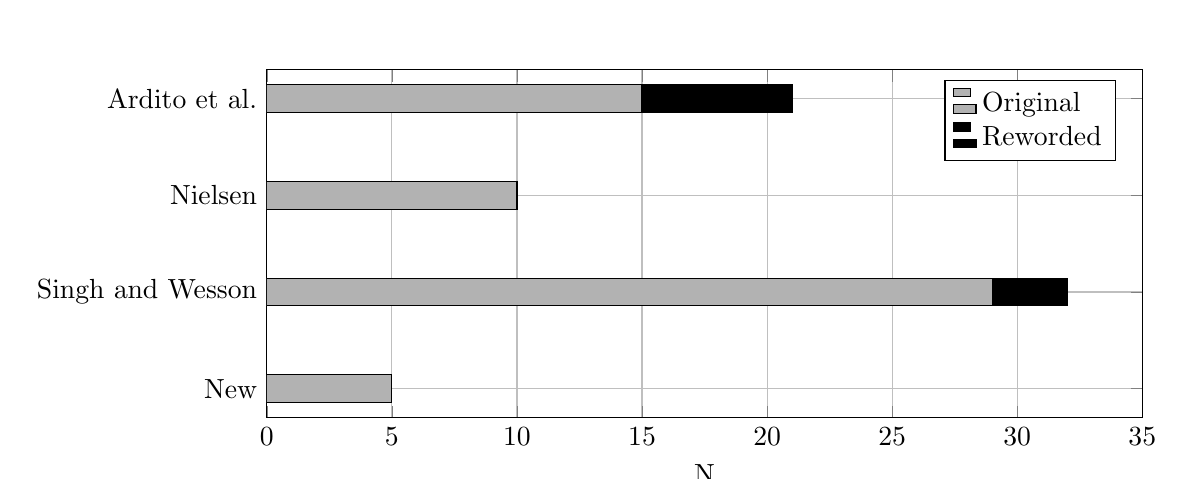
\begin{tikzpicture}
	\begin{axis} [
		height=6cm,
		xlabel=N,
		grid=major,
		legend pos=north east,
		legend cell align=left,
		xbar stacked,
		xmin=0,
		xmax=35,
		y dir=reverse,
		symbolic y coords={Ardito et al., Nielsen, Singh and Wesson, New},
	]
		\addplot[fill=black!30,xbar legend] coordinates {
			(15,Ardito et al.) (10,Nielsen) (29,Singh and Wesson) (5,New)
		};
		\addlegendentry{Original}
		
		\addplot[fill=black,xbar legend] coordinates {
			(6,Ardito et al.) (0,Nielsen) (3,Singh and Wesson) (0,New)
		};
		\addlegendentry{Reworded}
	\end{axis}
\end{tikzpicture}
	\caption{Sources of heuristics in usability experts' list}
	\label{img:first_final_list}
\end{figure}

\FloatBarrier
\section{Phase Two}
The second phase was administered between July 11th, 2012 and July 30th, 2012. The participants were asked to fill out an online questionnaire by rating the applicability of each of the heuristics from the first phase. The questionnaire also contained some background questions. After the participants filled out the questionnaire, the researcher called them to conduct a follow-up interview.

\subsection{Participants}
A total of six CRM users participated in this phase, although one of them could not be reached for the follow-up interview. All participants had at least two years of experience using a web-based CRM system. The mean number of years of experience was 5.67. With the exception of one participant, all use a CRM system daily. The other participant uses one two to three times per week. All but one of the participants had been using a web-based CRM system for the entirety of their years of experience with any CRM system. Table~\ref{tab:second_participants} gives on overview of the participants' experience.

\begin{table}[hbtp]
	\centering
	\vspace{0.5cm}
	\caption{Years of experience with CRM systems of the participants of the second phase}
	\begin{tabular}{lrrrrrr} \toprule
		& \multicolumn{6}{c}{\textbf{Participant}} \\
		\textbf{Years of Experience\ldots{}} & \textbf{F} & \textbf{G} & \textbf{H} & \textbf{I} & \textbf{J} & \textbf{K} \\ \midrule
		using a CRM system 				& 3 & 5 & 16 & 6 & 10 & 2 \\
		using a web-based CRM system	& 3 & 5 &  8 & 6 & 10 & 2 \\
		\bottomrule
	\end{tabular}
	\label{tab:second_participants}
\end{table}

Four of the participants used salesforce.com as their CRM system, one used a system called Bullhorn. The system the sixth participant used could not be determined.

\subsection{Evaluation of Usability Experts' Heuristics}
\label{sec:evaluation_existing_second}
The first activity in this phase, similarly to the first activity in the previous phase, consisted of a rating of the heuristics developed in the first phase based on their applicability to web-based CRM systems. The ratings were performed on a five-point scale ranging from ``not applicable'' (1) to ``highly applicable'' (5). There was an additional option of ``don't know'' for cases in which the participant was unable to understand the heuristic.

On average, it took the participants close to 52 minutes to complete the questionnaire. It should be noted that four of the participants took less than 45 minutes to complete the questionnaire, while it took the two others more than one hour.

A total of 68 heuristics was rated in this activity. Ten were taken from \citet{Nielsen1994a}, 32 from \citet{Singh2009}, 21 from \citet{Ardito2006}, and five were newly developed during the previous phase. Table~\ref{tab:second_results_bysource} shows selected descriptive statistics for the heuristics based on their source. Overall, the ratings of applicability were very similar and very high across all sources of heuristics. Appendix section~\ref{appsec:results_second} contains the detailed results of the rating activity.

\begin{table}[htbp]
	\centering
	\vspace{0.5cm}
	\caption{Overall applicability by heuristics source during second phase}
	\label{tab:second_results_bysource}
	\begin{tabular}{lrrrrrr} \toprule
			& & & \multicolumn4{c}{\textbf{Applicability}} \\
			\textbf{Source} & $\mathbf{N}$ & \textbf{\% Missing} & \textbf{Mean} & \textbf{Min.} & \textbf{Max.} & \textbf{St.\ Dev.} \\ \midrule
			\citet{Ardito2006} & 21 & 14.29 & 4.03 & 2 & 5 & 0.849 \\
			\citet{Nielsen1994a} & 10 & 10.00 & 4.08 & 1 & 5 & 0.614 \\
			\citet{Singh2009} & 32 & 4.69 & 4.33 & 2 & 5 & 0.699 \\
			New & 5 & 3.33 & 4.03 & 2 & 5 & 0.650 \\
		\bottomrule
	\end{tabular}
\end{table}

One exception is a heuristic which consistently received very low ratings by every participant. The heuristic is ``Users often choose system functions by mistake and will need a clearly marked `emergency exit' to leave the unwanted state without having to go through an extended dialogue. Support and undo and redo.'' by \citet{Nielsen1994a}. The mean rating for this heuristic was 1.83 with a standard deviation of 0.687. This is very surprising, as the usability experts rated this heuristic much higher, at 4.6 with a standard deviation of 0.894. Thus, this heuristic was one of the three which received the highest rating of applicability by the usability experts. This is by far the biggest distance between the ratings assigned by usability experts and CRM users for any one heuristic. Since the heuristic did receive very high ratings by the usability experts, it will remain in the list of accepted heuristics, until a measurement error can be eliminated as the reason for this discrepancy.

\begin{figure}[htbp]
	\centering
	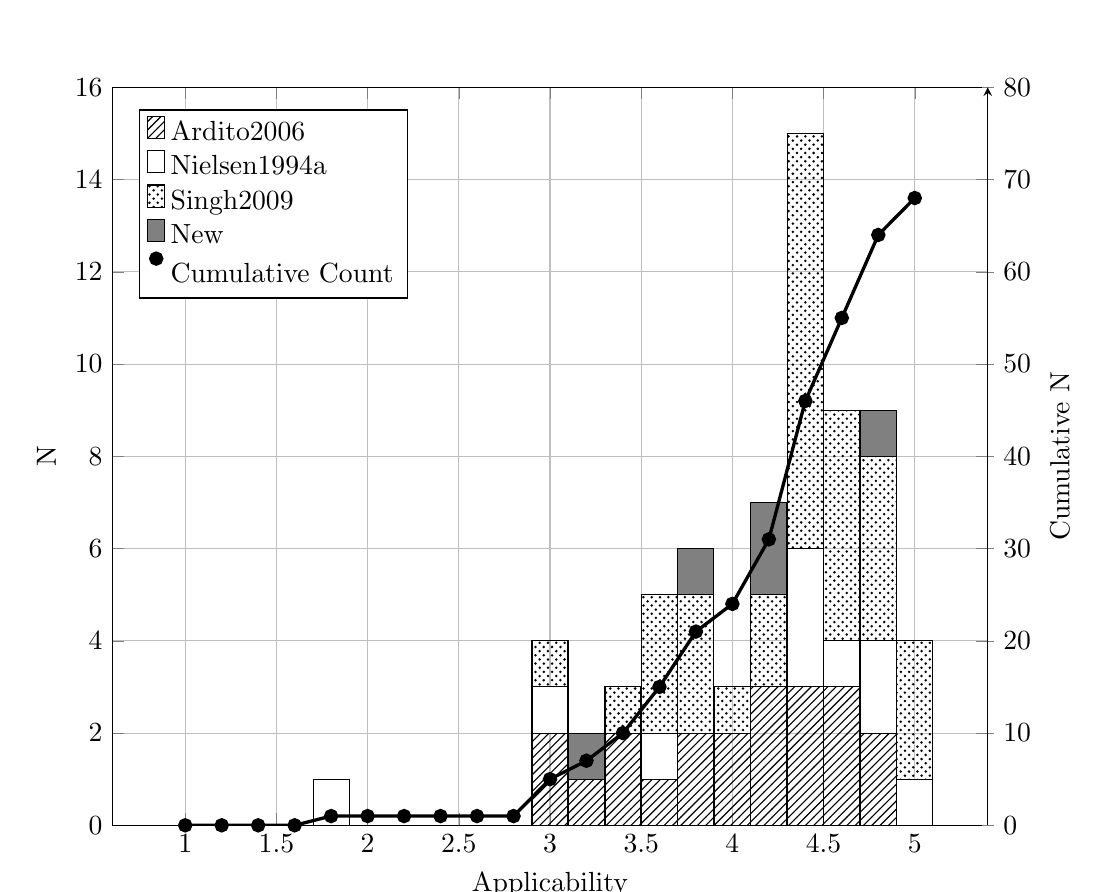
\begin{tikzpicture}
	\begin{axis} [
		xlabel=Applicability,
		ylabel=N,
		grid=major,
		legend pos=north west,
		legend cell align=left,
		ybar stacked,
		bar width=13pt,
		ymin=0,
		ymax=16
	]
		\addplot[fill=white,pattern=north east lines] coordinates {
			(1, 0) (1.2, 0) (1.4, 0) (1.6, 0) (1.8, 0) (2, 0) (2.2, 0) (2.4, 0) (2.6, 0) (2.8, 0) (3, 2) (3.2, 1) (3.4, 2) (3.6, 1) (3.8, 2) (4, 2) (4.2, 3) (4.4, 3) (4.6, 3) (4.8, 2) (5, 0)
		};
		\addlegendentry{\citet{Ardito2006}}
		
		\addplot[fill=white] coordinates {
			(1, 0) (1.2, 0) (1.4, 0) (1.6, 0) (1.8, 1) (2, 0) (2.2, 0) (2.4, 0) (2.6, 0) (2.8, 0) (3, 1) (3.2, 0) (3.4, 0) (3.6, 1) (3.8, 0) (4, 0) (4.2, 0) (4.4, 3) (4.6, 1) (4.8, 2) (5, 1)
		};
		\addlegendentry{\citet{Nielsen1994a}}
		
		\addplot[fill=white,pattern=crosshatch dots] coordinates {
			(1, 0) (1.2, 0) (1.4, 0) (1.6, 0) (1.8, 0)(2, 0) (2.2, 0) (2.4, 0) (2.6, 0) (2.8, 0) (3, 1) (3.2, 0) (3.4, 1) (3.6, 3) (3.8, 3) (4, 1) (4.2, 2) (4.4, 9) (4.6, 5) (4.8, 4) (5, 3)
		};
		\addlegendentry{\citet{Singh2009}}
		
		\addplot[fill=black!50] coordinates {
			(1, 0)  (1.2, 0) (1.4, 0) (1.6, 0) (1.8, 0) (2, 0) (2.2, 0) (2.4, 0) (2.6, 0) (2.8, 0) (3, 0) (3.2, 1) (3.4, 0) (3.6, 0) (3.8, 1) (4, 0) (4.2, 2) (4.4, 0) (4.6, 0) (4.8, 1) (5, 0)
		};
		\addlegendentry{New}
		
		\addlegendimage{sharp plot,mark=*,very thick}
		\addlegendentry{Cumulative Count}
	\end{axis}
	
	\begin{axis} [
		ylabel=Cumulative N,
		axis y line=right,
		axis x line=none,
		ybar,
		ymin=0,
		ymax=80
	]
		\addplot[sharp plot,mark=*,very thick] coordinates {
			(1, 0) (1.2, 0)(1.4, 0)  (1.6, 0) (1.8, 1) (2, 1) (2.2, 1) (2.4, 1) (2.6, 1) (2.8, 1) (3, 5) (3.2, 7) (3.4, 10) (3.6, 15) (3.8, 21) (4, 24) (4.2, 31) (4.4, 46) (4.6, 55) (4.8, 64) (5, 68)
		};
	\end{axis}
\end{tikzpicture}
	\caption{Count and cumulative count of heuristics based on applicability rating by CRM users}
	\label{img:second_cumulative}
\end{figure}

As adumbrated previously, the heuristics received much more uniform ratings in this phase than in the previous phase. When removing the outlier discussed in the previous paragraph, the lowest mean rating received by any heuristic in this phase is 3.0, which indicates relatively good applicability and the heuristics receiving this rating would have been included in the list of accepted heuristics in the previous phase. Figure~\ref{img:second_cumulative} shows the number of heuristics with a given rating of applicability as well as the cumulative count.

Another interesting figure is the percentage of abstentions for each group of heuristics. \citet{Ardito2006} received the highest number of missing votes, followed by \citet{Nielsen1994a}. Table~\ref{tab:second_results_bysource} shows the number of votes missing by source. The percentage represents the total number of votes missing. For \citet{Ardito2006}, the maximum number of votes that could have been cast is 21 heuristics times six participants ($21*6=126$). Of these, 18 votes have not been cast, leading to an abstention rate of 14.29\%. One likely interpretation of these figures is that the participants did not feel comfortable making a decision about the heuristics because they either were unable to understand the heuristic or because they did not feel they have enough experience to make a judgment. This could mean that the participants found the heuristics by \citet{Ardito2006} much harder to understand than the heuristics developed by the usability experts in the previous phase of the study. This problem was also present in phase one, where the participants stated that the most common problem with the heuristics was that they were difficult to understand.

\subsection{Oral Comments}
During this phase, five follow-up phone interviews were conducted with the participants. One participant could not be reached despite numerous attempts. Although the researcher attempted to perform the phone interviews shortly after the participants completed the questionnaire, this was not always possible. Only in two cases could the participants be reached within 24 hours of them completing the questionnaire. The other three participants were interviewed between six and sixteen days after their completing the questionnaire. The interviews consisted of three parts corresponding to the three subsections below.

\subsubsection{Introductory Questions}
The first two questions asked in the interview were focused on the CRM systems the participants use to create some context and get them to open up and become comfortable sharing their opinion. These questions were ``What do you like most about your CRM system?'' and ``What do you like least about your CRM system?''.

The participants were fairly open in discussing these topics and all had something positive and negative to say about their CRM systems without needing to reflect for a long period of time. Overall usability of the CRM systems was the most commonly named positive and negative aspect. Some of the participants found their respective CRM system very easy to use and user-friendly, while others thought theirs was difficult to use and required ``a lot of clicking around'' to complete a task. The participants who use salesforce.com reported that they liked their CRM system better than the participants who used another system.

Another common theme was the advantage of web-based systems to be available from anywhere, even mobile devices. One participant pointed out that she can access the system when working from home on her own computer and another participant said he loved the fact that he can look up information on the go from his smartphone. The participants also pointed out that they like the fact that their CRM system synchronizes across different communication tools such as e-mail clients. This was particularly important to one participant, whose company requires her to log all oral communications and store all written communications in their CRM system. Another participant mentioned that the information she has about her clients is synchronized between her CRM system and her e-mail client, so she can have access to that information from both systems.

Information overload was mentioned as a negative aspect of CRM systems as experienced by the users. One participant said he sometimes felt overwhelmed by the amount of information in the system and the speed at which it gets created, even though the system does provide categorization and filtering of the information.

\subsubsection{Overall Impression}
This section of the interview served to discuss the participants' overall impression of the heuristics as well as their opinion of whether any heuristics were missing or areas of CRM systems that had not been covered. The questions asked in this part of the interview were ``What was your overall impression of the heuristics you saw in the questionnaire?'' and ``Do you think there is anything that is important to CRM systems that was not covered by the heuristics?''.

The participants' overall impressions of the heuristics were good. They said that most of the heuristics seemed applicable and made sense to them. Some of the participants did point out that a number of the heuristics were ``wordy'' and difficult for them to understand, but that they selected the corresponding option on the questionnaire in those cases. Another participant stated that he was unable to judge some of the heuristics since he only had experience using the CRM system as opposed to administering it. This was especially true for heuristics related to customization, as this is often done by an administrator.

When asked whether they thought anything was missing, none of the participants identified an area. This question may have been problematic and not effective in uncovering missing heuristics, since humans are typically bad at identifying things that are missing when asked outright. Another explanation might be that most of the participants were satisfied with their CRM systems for the most part and therefore weren't able to identify potential usability problems, since they don't encounter them.

The participants did mention aspects of CRM systems they liked or disliked but which were not included in the heuristics. These aspects are \textit{access from mobile devices for traveling salespeople} and \textit{synchronization of data across communication tools} (e.g.\ contact information is automatically transferred to the e-mail client and communications with a contact are available from within the CRM system). Based on these two aspects, two new heuristics are added:
\begin{itemize}
	\item The system is accessible and usable from mobile devices.
	\item The system allows for synchronization of its information with outside communication tools.
\end{itemize}

\subsubsection{Focused Evaluation of New Heuristics}
Finally, special emphasis was placed on discussing the five heuristics which were developed in the first phase to create an extra layer of validation. In this section of the interview, the five newly created heuristics were read to the participants one by one and they were asked if they thought each particular heuristic was important for web-based CRM systems.

There was overall agreement among all participants that all heuristics are important to web-based CRM systems. Only in one case, one participant stated he didn't think the heuristic ``Help and documentation are immersed in the system, non-obtrusive, and ubiquitous'' was important, because he usually contacts his company's technical support team when he has a question about the CRM system, instead of consulting the system documentation.

\section{Comparative Analysis}
\subsection{Evaluation of Existing Heuristics}
As part of the final analysis, the ratings assigned by the usability experts and the CRM users were compared. Overall, the ratings for most heuristics were higher as assigned by CRM users than by usability experts. On average, the increase amounted to 0.55 points. The heuristics which were reworded by the usability experts received a much higher rating than the original heuristics. On average, the ratings for the reworded heuristics increased by 1.92 points as compared to the original heuristics. Table~\ref{tab:rating_difference_bysource} shows the difference in ratings between phases by source.

\begin{table}[htbp]
	\centering
	\vspace{0.5cm}
	\caption{Comparison of rating differences between phases by source}
	\label{tab:rating_difference_bysource}
	\begin{tabular}{lccc}	\toprule
		\textbf{Source} & \textbf{Usability Experts} & \textbf{CRM Users} & \textbf{Difference} \\ \midrule
		\citet{Ardito2006} 		& 3.19 	& 4.03 &  0.84 	\\
		\citet{Nielsen1994a} 	& 4.10 	& 4.08 & -0.02 	\\
		\citet{Singh2009} 		& 3.79 	& 4.33 &  0.54 	\\
		New 					&  ---	& 4.03 &   ---	\\
		\bottomrule
	\end{tabular}
\end{table}

Of the five heuristics whose rating decreased the most between the two phases, the average decrease was 1.3 points. Three of these heuristics were developed by \citet{Nielsen1994a}. Table~\ref{tab:biggest_losers} gives an overview of these five heuristics. The five heuristics which experience the largest increase in ratings are shown in table~\ref{tab:biggest_winners_overall}. All of these heuristics are reworded versions of the original heuristics. Table~\ref{tab:biggest_winners_original} shows the five heuristics which received the highest increase in ratings when excluding the reworded heuristics.

\begin{table}[htbp]
	\centering
	\vspace{0.5cm}
	\caption{Heuristics whose applicability rating decreased by 0.8 points or more during phase two}
	\label{tab:biggest_losers}
	\begin{tabularx}{\textwidth}{Xcc}	\toprule
		\textbf{Heuristic} & \textbf{Source} & \textbf{Difference} \\ \midrule
		Users often choose system functions by mistake and will need a clearly marked `emergency exit' to leave the unwanted state without having to go through an extended dialogue. Support and undo and redo. & N & -2.77 \\
		The ability of the UI to be configured without affecting the underlying business logic of the system & S & -1.4 \\
		Accelerators -- unseen by the novice user -- may often speed up the interaction for the expert user to such an extent that the system can cater to both inexperienced and experienced users. Allow users to tailor frequent actions. & N & -0.8 \\
		Introduce mechanism to highlight errors and cues to avoid errors & A & -0.8 \\
		Dialogues should not contain information which is irrelevant or rarely needed. Every extra unit of information in a dialogue competes with the relevant units of information and diminishes their relative visibility. & N & -0.8 \\
		\bottomrule
	\end{tabularx}
\end{table}

\begin{table}[htbp]
	\centering
	\vspace{0.5cm}
	\caption{Heuristics with the largest rating increase}
	\label{tab:biggest_winners_overall}
	\begin{tabularx}{\textwidth}{Xcc}	\toprule
		\textbf{Heuristic} & \textbf{Source} & \textbf{Difference} \\ \midrule
			Clearly visualize employee performance & A & 2.83 \\
			Highlight cross-references between different types of data (e.g.\ customer issues, sales support, and marketing campaigns) & A & 2.63 \\
			Clearly visualize user workflow & A & 2.33 \\
			The system reduces intimidation and complexity by providing positive feedback and reinforcement, a clear path to execution, and a terminology that matches the users' language & S & 2.27 \\
			The system's communication mechanisms match the needs of the users & A & 2.17 \\
		\bottomrule
	\end{tabularx}
\end{table}

\begin{table}[htbp]
	\centering
	\vspace{0.5cm}
	\caption{Heuristics with the largest rating increase excluding reworded heuristics}
	\label{tab:biggest_winners_original}
	\begin{tabularx}{\textwidth}{Xcc}	\toprule
		\textbf{Heuristic} & \textbf{Source} & \textbf{Difference} \\ \midrule
			Functionality to search for information that is available & S & 1.6 \\
			The output provided provides clear visibility into the various other departments & S & 1.5 \\
			Clearly visualize progress tracking & A & 1.4 \\
			Maximize adaptation of technology to the context of use & A & 1.33 \\
			The system improves user productivity & S & 1.07 \\
		\bottomrule
	\end{tabularx}
\end{table}

\FloatBarrier
\subsection{Creation of New Heuristics}
During phase one, five new heuristics were created and then accepted by the participants in phase two.
\begin{enumerate}
	\item The system provides appropriate filters to organize data
	\item The system allows for tailoring of the interface to an individual's workflow
	\item The system displays appropriate information depending on the task at hand
	\item The system has a dashboard which shows the current status at a quick glance
	\item Help and documentation are immersed in the system, non-obtrusive, and ubiquitous	
\end{enumerate}

During phase two, two new heuristics were added.
\begin{enumerate}
	\setcounter{enumi}{5}
	\item The system is accessible and usable from mobile devices
	\item The system allows for synchronization of its information with outside communication tools
\end{enumerate}

To create a unified list of heuristics in appropriate categories, these seven heuristics can be added to the categories created by \citet{Singh2009}. Heuristics 1, 3, 4, and 7 can be sorted into the category \textit{task support}, 2 can be added to \textit{customization}, 6 belongs to \textit{presentation}, and 5 belongs to \textit{learnability}.

The ten heuristics developed by \citet{Nielsen1994a} can also be sorted into the categories developed by \citet{Singh2009} to create a single list of heuristics for web-based CRM systems. See table~\ref{tab:nielsen_to_singh} for the categorization of the heuristics.

\begin{table}[htbp]
	\centering
	\caption{Categorizing heuristics developed by \citet{Nielsen1994a} into categories developed by \citet{Singh2009}}
	\label{tab:nielsen_to_singh}
	\begin{tabularx}{\textwidth}{Xc} \toprule
		\textbf{Heuristic} & \textbf{Category} \\ \midrule
		Even though it is better if the system can be used without documentation, it may be necessary to provide help and documentation. Any such information should be easy to search, focused on the user's task, list concrete steps to be carried out, and not be too large. & Learnability \\
		Even better than good error messages is a careful design which prevents a problem from occurring in the first place. & Navigation \\
		Make object, actions, and options visible. The user should not have to remember information from one part of the dialogue to another. Instructions for use of the system should be visible or easily retrievable whenever appropriate. & Navigation \\
		Accelerators -- unseen by the novice user -- may often speed up the interaction for the expert user to such an extent that the system can cater to both inexperienced and experienced users. Allow users to tailor frequent actions. & Navigation \\
		The system should always keep users informed about what is going on, through appropriate feedback within reasonable time. & Presentation \\
		Dialogues should not contain information which is irrelevant or rarely needed. Every extra unit of information in a dialogue competes with the relevant units of information and diminishes their relative visibility. & Presentation \\
		Error messages should be expressed in plain language (no codes), precisely indicate the problem, and constructively suggest a solution. & Presentation \\
		The system should speak the users' language with words, phrases, and concepts familiar to the user, rather than system-oriented terms. Follow real-world conventions, making information appear in a natural and logical order. & Task Support \\
		Users often choose system functions by mistake and will need a clearly marked ``emergency exit'' to leave the unwanted state without having to go through an extended dialogue. Support and undo and redo. & Task Support \\
		Users should not have to wonder whether different words, situations, or actions mean the same thing. Follow platform conventions. & Task Support \\
		\bottomrule
	\end{tabularx}
\end{table}

\FloatBarrier
Most of the remaining heuristics by \citet{Ardito2006} can remain in their categories and are added to the final list of heuristics. Solely the two heuristics that were in the category \textit{hypermediality} are added to the category \textit{task support} instead, since it is a better fit for them. Finally, the list of heuristics for web-based CRM systems consists of the categories and heuristics displayed in table~\ref{tab:final_list}. There are a total of 70 heuristics in seven categories. Table~\ref{tab:final_list_composition} shows the composition of the final list.

\begin{table}[htbp]
	\centering
	\vspace{0.5cm}
	\caption[Composition of the final list of heuristics]{Composition of the final list of heuristics; N = \citet{Nielsen1994a}, S = \citet{Singh2009}, A = \citet{Ardito2006}}
	\label{tab:final_list_composition}
	\begin{tabular}{lcccc|c} \toprule
		\textbf{Category} & \textbf{N} & \textbf{S} & \textbf{A} & \textbf{New} & \textbf{Total} \\ \midrule
		Application Proactivity	&  0 &  0 &  6 & 0 &  6 \\
		Customization 			&  0 &  5 &  0 & 1 &  6 \\
		Learnability 			&  1 &  5 &  0 & 1 &  7 \\
		Navigation 				&  3 &  8 &  0 & 0 & 11 \\
		Presentation 			&  3 &  6 &  8 & 1 & 18 \\
		Task Support 			&  3 &  8 &  2 & 4 & 17 \\
		User Activity 			&  0 &  0 &  5 & 0 &  5 \\ \midrule
		\textbf{Total} 			& 10 & 32 & 21 & 7 & 70 \\
		\bottomrule
	\end{tabular}
\end{table}

\begin{singlespace}
		\tabulinesep=_1mm^1mm
	\begin{longtabu} to \textwidth {l X[1, p] c}
			\label{tab:final_list}\\
			\caption{Final, unified list of heuristics for web-based CRM systems}\\
			\toprule
			\textbf{Category} & \textbf{Heuristic} & \textbf{Source} \\
			\midrule
		\endfirsthead
			
			\textbf{Category} & \textbf{Heuristic} & \textbf{Source} \\
			\midrule
		\endhead
		
			\bottomrule
		\endlastfoot
		
		Application Proactivity & Introduce mechanisms to prevent usage errors & A \\
		Application Proactivity & Maximize adaptation of technology to the context of use & A \\
		Application Proactivity & Provide mechanisms for teaching-through-er\-rors & A \\
		Application Proactivity & Provide mechanisms to manage user's profiles & A \\
		Application Proactivity & Register the date of last modification of documents to facilitate updating & A \\
		Application Proactivity & The system conforms to platform conventions & A \\
		Customization & The ability of the system to be re-configured over a period of time & S \\
		Customization & The ability of the UI to be configured without affecting the underlying business logic of the system & S \\
		Customization & The alignment of the system to update existing business processes, and (or) to include new ones & S \\
		Customization & The capability of the system to support user-level customization & S \\
		Customization & The ease in which the system can be configured to a particular industry type & S \\
		Customization & The system allows for tailoring of the interface to an individual's workflow & New \\
		Learnability & A user can learn how to use the system without a long introduction & S \\
		Learnability & Even though it is better if the system can be used without documentation, it may be necessary to provide help and documentation. Any such information should be easy to search, focused on the user's task, list concrete steps to be carried out, and not be too large. & N \\
		Learnability & Help and documentation are immersed in the system, non-obtrusive, and ubiquitous & New \\
		Learnability & It is easy to become skillful at using the system within a short amount of time & S \\
		Learnability & The system reduces intimidation and complexity by providing positive feedback and reinforcement, a clear path to execution, and a terminology that matches the users' language & S \\
		Learnability & The various functions of the system can be identified by exploration & S \\
		Learnability & There is sufficient on-line help to support the learning process & S \\
		Navigation & Accelerators -- unseen by the novice user -- may often speed up the interaction for the expert user to such an extent that the system can cater to both inexperienced and experienced users. Allow users to tailor frequent actions. & N \\
		Navigation & Even better than good error messages is a careful design which prevents a problem from occurring in the first place. & N \\
		Navigation & Functionality can be found quickly and easily & S \\
		Navigation & Functionality to search for information that is available & S \\
		Navigation & Information can be easily accessed & S \\
		Navigation & Make object, actions, and options visible. The user should not have to remember information from one part of the dialogue to another. Instructions for use of the system should be visible or easily retrievable whenever appropriate. & N \\
		Navigation & The results returned by a search are relevant to the information required by the user & S \\
		Navigation & The system can guide the user through the correct sequence of transaction to complete a business process & S \\
		Navigation & The system is capable of supporting the different interaction styles of the various users & S \\
		Navigation & The UI supports efficient and accurate navigation of the system & S \\
		Navigation & There is clarity in terms of the next sequence of transactions of steps & S \\
		Presentation & Clearly and constantly indicate system state & A \\
		Presentation & Clearly visualize employee performance & A \\
		Presentation & Clearly visualize options and commands available & A \\
		Presentation & Clearly visualize progress tracking & A \\
		Presentation & Clearly visualize user workflow & A \\
		Presentation & Dialogues should not contain information wh\-ich is irrelevant or rarely needed. Every extra unit of information in a dialogue competes with the relevant units of information and diminishes their relative visibility. & N \\
		Presentation & Error messages should be expressed in plain language (no codes), precisely indicate the problem, and constructively suggest a solution. & N \\
		Presentation & Introduce mechanism to highlight errors and cues to avoid errors & A \\
		Presentation & Maintain UCD [user-centered design] at\-trib\-utes for interface graphical aspects & A \\
		Presentation & The information presented supports informed decision making & S \\
		Presentation & The information provided by the system is timely, accurate, complete and understandable & S \\
		Presentation & The output provided provides clear visibility into the various other departments & S \\
		Presentation & The output style fits the type of data being displayed & S \\
		Presentation & The system is accessible and usable from mobile devices & New \\
		Presentation & The system is customizable at the user level & A \\
		Presentation & The system should always keep users informed about what is going on, through appropriate feedback within reasonable time. & N \\
		Presentation & The UI [user interface] is intuitive & S \\
		Presentation & The visual layout is well designed & S \\
		Task Support & Highlight cross-references between different ty\-pes of data (e.g. customer issues, sales support, and marketing campaigns) & A \\
		Task Support & Supply different media channels for communication & A \\
		Task Support & The information provided by the system is in real-time & S \\
		Task Support & The responses from the system are quick and efficient & S \\
		Task Support & The system allows for synchronization of its information with outside communication tools & New \\
		Task Support & The system automates routine and redundant tasks & S \\
		Task Support & The system displays appropriate information depending on the task at hand & New \\
		Task Support & The system has a dashboard which provides a quick glance of the current status & New \\
		Task Support & The system improves user productivity & S \\
		Task Support & The system is easy to use & S \\
		Task Support & The system provides appropriate filters to organize data & New \\
		Task Support & The system should speak the users' language with words, phrases, and concepts familiar to the user, rather than system-oriented terms. Follow real-world conventions, making information appear in a natural and logical order. & N \\
		Task Support & The system supports efficient completion of tasks & S \\
		Task Support & The system supports improved information flow between the various organizational departments & S \\
		Task Support & The terminology used by the system is consistent with the terminology of the user & S \\
		Task Support & Users often choose system functions by mistake and will need a clearly marked "emergency exit" to leave the unwanted state without having to go through an extended dialogue. Support and undo and redo. & N \\
		Task Support & Users should not have to wonder whether different words, situations, or actions mean the same thing. Follow platform conventions. & N \\
		User Activity & Insert mechanisms to make annotations & A \\
		User Activity & Provide both synchronous and asynchronous communication tools & A \\
		User Activity & Provide easy-to-use authoring tools & A \\
		User Activity & Provide mechanisms for search by indexing, key or natural language & A \\
		User Activity & The system's communication mechanisms mat\-ch the needs of the users & A \\
	\end{longtabu}
\end{singlespace}

\chapter{Discussion \& Conclusion}
\label{chap:discussion}
The purpose of this study was to identify the usability heuristics relevant to web-based CRM systems. To investigate this problem, a two-phased study was conducted involving both usability experts and CRM users. While the previous chapter presented the results of the two phases as well as the comparative analysis, this chapter presents a discussion of the results and the findings gleaned from them, as well as their implications and the study's limitations.

\section{Discussion}
\subsection{Applicability Based on Specificity}
The results of the first phase showed a gradation in applicability of the heuristics based on their source. The most general set of heuristics \citep{Nielsen1994a} received the highest ratings at 4.087, followed closely by the heuristics specifically developed for ERP systems \citep{Singh2009} at 4.086 points, while the heuristics for e-learning systems \citep{Ardito2006} received the lowest ratings at 3.647 points. The reason for this may be that the general heuristics were not developed with a specific class of applications in mind. They were intentionally created to be applicable to a wide array of user interfaces \citep[p.\ 28]{Nielsen1994a}.

On the other hand, previous research has shown that some usability problems may be missed, if only general heuristics are used in an evaluation \citep[e.g.][]{Rusu2011}, so it is necessary to create heuristics for specific applications to improve usability evaluations, even though they may not be widely applicable.

\subsection{Applicability Based on Domain}
The ERP heuristics were likely rated as more applicable than the e-learning heuristics, because ERP systems are more similar to CRM systems. In fact, many ERP systems contain CRM systems. They also support similar work flows and users, as opposed to e-learning systems, which have a different audience and goals. ERP and CRM systems are usually used to support and even automate business processes, while e-learning systems are used to support learning processes and education.

This finding shows that similar classes of applications share more of the same heuristics than applications used for very different purposes. This finding also supports previous research indicating that different heuristics are needed to appropriately cover different classes of applications \citep[e.g.][]{Rusu2011}. In addition, the \textit{Task-Technology Fit} model discussed in section~\ref{sec:ttf} shows that task characteristics have a direct influence on task-technology fit. Two tasks with very different characteristics will likely also have a different technology fit, whereas tasks which share many characteristics and are more similar will have a similar fit to a technology.

\subsection{Lack of Specificity of Usability Experts' New Heuristics}
The five new heuristics developed by the usability experts in phase one are relatively general and do not use any domain-specific terminology. They appear to be applicable to a variety of systems that are used to store and access large volumes of information and support business processes.

The reason for this lack of specificity may be that most of the usability experts had very little experience with CRM systems. On average, the participants had only 1.2 years of experience using a CRM system. \Citet{Nielsen1992} found that in heuristic evaluations, evaluators who have expertise in both usability as well as the subject matter of the system being evaluated find 19 percentage points more usability problems than evaluators who do not have subject matter expertise. It is quite likely that the participants in this thesis study had difficulty developing heuristics that are more specific to CRM systems because they were not ``double specialists''. This limitation is discussed in greater detail in section~\ref{sec:limitations}.

\subsection{Differences in Ratings for \citeauthor{Nielsen1994a}'s Heuristics}
On average, the usability experts rated the heuristics developed by \citet{Nielsen1994a} higher than the CRM users did. The average applicability rating assigned to \citeauthor{Nielsen1994a}'s heuristics (4.10) by usability experts is 0.81 higher than the average rating for all heuristics (3.29). On the contrary, the average rating assigned to \citeauthor{Nielsen1994a}'s heuristics (4.08) by CRM users is 0.10 points lower than the average rating for all heuristics (4.18). This means that the usability experts considered \citeauthor{Nielsen1994a}'s heuristics more applicable and important than the CRM users did.

Based on observations made during the focus group discussion, it is likely that most of the usability experts recognized these heuristics and their importance in the field of usability research, while none of the CRM users did. Since the usability experts recognized \citeauthor{Nielsen1994a}'s importance in the field, which became evident in the focus group discussion, they may have been biased to assigning a higher rating to his heuristics than they actually deserved.

It is also possible that the CRM users assigned lower ratings to \citeauthor{Nielsen1994a}'s heuristics, because they are general in nature and the participants therefore thought they were less useful than the more specific heuristics.

\subsection{Low Rating for \textit{User Control and Freedom} Heuristic by CRM Users}
One of \citeauthor{Nielsen1994a}'s heuristics (``Users often choose system functions by mistake and will need a clearly marked `emergency exit' to leave the unwanted state without having to go through an extended dialogue. Support undo and redo.'') received a particularly high rating by the usability experts, while the CRM users assigned the lowest rating by far to it.

One possible explanation is the previously mentioned bias of the usability experts to rate this heuristic highly, although it may not be very applicable in reality. This explanation seems possible, yet is unlikely, because there is such a big discrepancy between the two ratings.

Another explanation might be that the users took offense to the wording of the heuristic, thinking that they do not, in fact, make a lot of mistakes when using a system. It is also possible that the users had trouble understanding this particular heuristic, as they assigned higher ratings to other heuristics related to error avoidance and recovery (``Introduce mechanisms to prevent usage errors'' received a rating of 4.6, ``Introduce mechanisms to highlight errors and cues to avoid errors'' received a rating of 3.0). Further research is necessary to investigate this discrepancy.

\subsection{Answers to Research Questions}
The first research question, ``What are the usability heuristics relevant to web-based CRM systems?'' was answered by the creation of the unified list in table~\ref{tab:final_list}. Existing heuristics were evaluated by two sets of participants and those with high ratings of applicability to web-based CRM systems were included in the final list. It contains heuristics from four sources: the heuristics created by \citet{Nielsen1994a}, \citet{Singh2009}, and \citet{Ardito2006}, as well as heuristics created by the participants of the study.

The answer to the second research question, ''Which heuristics are irrelevant?'', shows that heuristics are irrelevant to a particular class of applications, if they contain domain-specific wording or references to user interface elements, which are not used in the class of applications at hand. More broadly-formulated, general heuristics are applicable to more classes of applications, but less helpful in identifying domain-specific usability problems.

The final research question, ``Are there new heuristics that need to be added?'', can be answered with a ``yes''. Seven new heuristics were created during the study and added to the body of heuristics for web-based CRM systems. It is expected that these heuristics are most relevant to web-based CRM systems and less relevant to other types of computer systems.

\section{Contributions}
This study was the first to investigate usability heuristics for web-based CRM systems as well as the effects of the involvement of users in the process of developing domain-specific usability heuristics. It was shown that there is a difference in the applicability of a set of heuristics based on the domain it is applied to. General heuristics remain largely applicable to specific domains, while the applicability of specific heuristics depends on the similarity of the domain they were developed for and the one they are used to evaluate.

The findings of this study demonstrate that users can be involved in the process of developing domain-specific heuristics and can add subject matter expertise, especially if the usability experts have no or only limited experience with the specific class of applications. It was shown that people unfamiliar with usability evaluations and heuristics are still able to understand them for the most part and can make valuable contributions and judgments on their applicability to a domain they are familiar with.

\section{Implications}
\subsection{For Research}
The results of this study show that there is a need for developing domain-specific usability heuristics for the various classes of software in use. It will also be necessary to periodically evaluate existing heuristics to investigate whether they need to be adapted to account for emerging types of systems.

Since this study found that even people untrained in usability evaluations can understand heuristics and make contributions to the development of them, the question of whether usability experts are still necessary arises. Traditionally, usability experts both create usability heuristics and then use them to evaluate software and identify usability problems. Now that non-experts were successfully included in the development of new heuristics, it remains to be answered whether this holds true in general and usability experts do not have to play the main role in developing new heuristics, but can inform the process and support domain experts in the development. It is also possible that the non-experts could perform a heuristic evaluation by themselves and apply a set of defined heuristics correctly to identify usability problems.

There are also implications with regard to the two theories discussed in section~\ref{sec:theories}. Some of the constructs contained in these models have relationships with the concepts and findings developed in this thesis.

\subsubsection{IS Success Model}
The study performed in this thesis mostly relates to the independent variables in the IS Success Model, as these capture the quality of the system, information, and service, rather than the attitudes and behaviors which are captured by the dependent variables. Usability heuristics are used to improve the quality of an information system, which will then influence the attitudes and behaviors.

\paragraph{System quality} measures the desired characteristics of the information system itself \citep{DeLone2004}. Among these qualities are usability, availability, and reliability. \textit{System flexibility} is also one of the characteristics included in \textit{system quality} and was originally developed by \citet{Hamilton1981a}. In the final list of heuristics developed in the present study, there are thirteen items related to flexibility and customizability, which is a component of flexibility (see table~\ref{tab:flexibility_heuristics}).

\begin{table}[htb]
	\vspace{0.5cm}
	\centering
	\caption{Heuristics related to system flexibility with overall applicability ratings}
	\label{tab:flexibility_heuristics}
	\begin{tabularx}{\textwidth}{Xcc} \toprule
		\textbf{Heuristic} & \textbf{Source} & \textbf{Applicability} \\ \midrule
		Maximize adaptation of technology to the context of use & A & 3.73 \\
		Provide mechanisms for search by indexing, key or natural language & A & 3.93 \\
		Supply different media channels for communication & A & 3.82 \\
		The system is customizable at the user level & A & 3.00 \\
		The system's communication mechanisms match the needs of the users & A & 3.18 \\
		Accelerators -- unseen by the novice user -- may often speed up the interaction for the expert user to such an extent that the system can cater to both inexperienced and experienced users. Allow users to tailor frequent actions. & N & 3.96 \\
		The system allows for tailoring of the interface to an individual's workflow & New & 3.17 \\
		The system is accessible and usable from mobile devices & New & --- \\
		The ability of the system to be re-configured over a period of time & S & 4.13 \\
		The ability of the UI to be configured without affecting the underlying business logic of the system & S & 3.64 \\
		The capability of the system to support user-level customization & S & 3.55 \\
		The ease in which the system can be configured to a particular industry type & S & 3.89 \\
		The system is capable of supporting the different interaction styles of the various users & S & 3.64 \\
		\bottomrule
	\end{tabularx}
\end{table}

These heuristics generally recommend that the system be flexible to allow for varying interaction modes across users as well as for customization of the system to different users, business processes, and industries. Since there is a total of 70 heuristics in the list, the percentage of heuristics relating to system flexibility is 18.6\%. This finding reinforces the relationship between usability and system quality.

\paragraph{Information quality} measures the quality of the information system's output \citep{DeLone1992}. This construct contains measures such as relevance, understandability, accuracy, and timeliness of the information provided by the system. There are nine items in the final list of heuristics developed in the present study relating to information quality (see table~\ref{tab:iq_heuristics}). The heuristics are concerned with clarity, relevance, usableness, and timeliness of the system's output. This shows that information quality is important for the usability of CRM systems.

\begin{table}[htb]
	\vspace{0.5cm}
	\centering
	\caption{Heuristics related to information quality with overall applicability ratings}
	\label{tab:iq_heuristics}
	\begin{tabularx}{\textwidth}{Xcc} \toprule
		\textbf{Heuristic} & \textbf{Source} & \textbf{Applicability} \\ \midrule
		Clearly visualize employee performance & A & 3.55 \\
		The system displays appropriate information depending on the task at hand & New & 4.17 \\
		The system has a dashboard which provides a quick glance of the current status & New & 4.83 \\
		The system allows for synchronization of its information with outside communication tools & New & --- \\
		Information can be easily accessed & S & 4.55 \\
		The information presented supports informed decision making & S & 4.53 \\
		The information provided by the system is in real-time & S & 4.18 \\
		The information provided by the system is timely, accurate, complete and understandable & S & 4.73 \\
		The output provided provides clear visibility into the various other departments & S & 3.82 \\
		The output style fits the type of data being displayed & S & 4.15 \\
		\bottomrule
	\end{tabularx}
\end{table}

\paragraph{Service quality} is a construct focused on the support the information system and IS organization provides for end users and includes \textit{tangibility}, \textit{reliability}, \textit{responsiveness}, \textit{assurance}, and \textit{empathy} \citep{DeLone2003}. With regard to this thesis, two instruments in this construct are of particular interest, \textit{responsiveness} (promptness of service to users) and \textit{assurance} (knowledge of IS employees to do their job well). During the phone interviews performed with CRM users, one of the participants pointed out that help and documentation are not important to him, because he prefers to consult the IT department when he has a question about or problem with the CRM application instead of reading the help documentation. It seems reasonable to assume that this attitude is fairly common among end users and therefore, a responsive and knowledgeable IT help desk are important in ensuring the success of an information system.

This discovery shows that there is a relationship between service quality and usability, as increased service quality through a responsive and competent help desk can increase the ability of the end users to properly operate the system and therefore increase \textit{user satisfaction} with the system. There is also an interesting implication when looking at the relationship in the opposite direction. A good help desk could effectively erase the need for good documentation of the system for some users, although others may still prefer to use the documentation instead of consulting the help desk.

\subsubsection{Task-Technology Fit}
The results of the study performed for this thesis have implications for the three variables in the task-technology fit model developed by \citet{Goodhue1995}.

\paragraph{Task characteristics} are the characteristics of the ``actions carried out by individuals in turning inputs into outputs'' \citep{Goodhue1995}. Tasks can be classified by their variety and difficulty, interdependence, and routineness \citep{Goodhue1995}. The different tasks performed within CRM systems can be classified into different groups. Answering a customer's complaint call, for example, entails more variety and less interdependence, than creating a report about the sales performance of products across market segments. There are also differences in classification of tasks from different classes of systems. The characteristics of the tasks performed with an accounting system likely differ from those performed with a CRM system.

\paragraph{Technology characteristics} are the characteristics of the ``tools used by individuals in carrying out their tasks''. While an examination of the tools/systems themselves was not part of this study, previous research has examined CRM systems. \Citet{Band2010,Band2010a}, for example, compared the functionality and usability of a variety of CRM systems and found a number of differences.

\paragraph{Task-technology fit} is ``the extent that technology functionality matches task requirements and individual abilities''. The findings of this thesis study show that the more similar the task characteristics are, the more applicable the heuristics are. This finding is in line with the idea that task-technology fit will be similar for tasks which share many characteristics when using the same technology.

\subsection{For Practice}
For practitioners, the findings of this study show that it is indeed important to use both general heuristics and heuristics specific to the class of system being evaluated, as other heuristics are not as applicable. If there is not a set of heuristics specific to the type of system being evaluated, it should be developed. Alternatively, it may be acceptable to use a set of heuristics for a similar type of applications, as this study shows that heuristics for similar types of applications are more applicable than heuristics for very different types of applications. In addition, the set of heuristics developed in this study can be used for heuristic evaluations of web-based CRM systems.

Second, this study has shown that users of the software heuristics are being developed for can be involved in the process successfully. They can add a domain-specific perspective to the development of heuristics, especially when the usability experts do not have that experience. It remains to be answered whether usability experts are even still needed for heuristic evaluations, as it has been shown that users can understand them, although it has not been proven that they know how to apply the heuristics to identify usability problems. This implication could change the role of the usability expert to be someone who informs and guides the development of heuristics and their application.

\section{Limitations}
\label{sec:limitations}
The biggest limitation of this study is its small sample size. Typically, it is recommended to repeat focus groups on a particular topic at least three or four times with different participants to ensure as many points as possible are covered \citep{Edmunds1999,Morgan1998}. Due to time constraints, this was not possible. Instead, the second phase of this study was used to achieve a degree of validity by engaging CRM users.

This means the results only have limited generalizability and thus external validity \citep[p.\ 158]{Creswell1994}. In addition, reproducibility of the results may be limited due to the qualitative and exploratory nature of the study as well as the small sample size, which can lead to decreased reliability \citep[p.\ 159]{Creswell1994}.

With regard to the participants themselves, there were two main limitations. First, the participants in phase one had expertise in usability engineering, but not in using or designing CRM systems (i.e.\ they were not ``double experts''). This means that they had a sub-optimal understanding of the characteristics of CRM systems and the tasks performed on them, which manifested itself during the creation of new heuristics, because their lack of domain-specific knowledge led to the development of less specific heuristics.

Second, the participants of the second study were difficult to recruit. Initially, the researcher planned to perform two focus group sessions (with the same protocol), but due to a lack of participants available at any single point in time, it became necessary to switch to the method described in this study.

This change brought with it another limitation. The participants were not briefed in person about the purpose of the study and their role in it. They merely received a written set of instructions and explanations. It is expected that some participants may not have read these instructions and explanations in full detail and thus did not understand their role in the study as fully as others.

Another limitation during this phase was that in many cases, more than a week passed between the point in time when participants filled out the questionnaire and when they could be reached for the follow-up interview. This means these participants did not have the questionnaire fresh on their minds. To mitigate this limitation, a few engagement questions were asked to refocus the participants on the topic and make them more comfortable expressing their opinion (see section~\ref{sec:session_structure}). Yet, it would have been beneficial to interview all participants within 24 or 48 hours after they filled out the questionnaire.

\section{Future Directions}
\label{sec:future_research}
Due to the limitations faced by this study outlined above, a future research direction is the validation of the results with a greater sample of usability experts and CRM users. This could be accomplished through a method similar to that used in this thesis, e.g.\ through repeated collaborative sessions.

Alternatively, a quantitative methodology for the validation of the results could be developed to be able to capture the judgment of a greater number of participants and analyze the results using more advanced statistical methods. This new methodology could be similar to the questionnaire used in the second phase of this study.

Furthermore, the usefulness of the developed set of heuristics has not been researched. Future research could investigate the usefulness of the heuristics for user interface designers etc.\ seeking to perform a heuristic evaluation of a web-based CRM system.

It would also be interesting to investigate the discrepancy in ratings for the \textit{user control and freedom} heuristic to find out why this heuristic was rated as highly applicable by usability experts and very inapplicable by CRM users.

Another interesting research area would be the success of involving of non-usability experts in the use of heuristics. While this study has shown that non-usability experts can understand heuristics and make valuable contributions in judging their applicability to a domain they are familiar with, it is unclear whether they would be able to apply them in an evaluation to identify usability problems. It would also be interesting to investigate whether heuristics can be successfully evaluated by non-usability experts alone, effectively removing the need for usability experts entirely.

Finally, a generalizable framework for developing usability heuristics for a specific class of applications should be developed, so that new heuristics can be developed more easily and reliably. This framework could be based on the method used in this study.

\section{Conclusion}
\label{sec:conclusions}
This thesis investigated usability heuristics and their applicability to web-based CRM systems. A literature review and research method were presented to address the questions:

\RQ{}

A two-phased, mixed approach combining different qualitative and quantitative methods was employed to answer the research questions.

With regard to the first two research questions, general heuristics were found to be more applicable to this specific class of applications than heuristics developed for other classes of systems which are used for purposes that greatly differ from CRM systems. Heuristics for e-learning systems, for example, were shown to be much less applicable than the general heuristics developed by \citet{Nielsen1994a}.

As for the third research questions, there were seven new heuristics, which were created specifically for web-based CRM systems. This shows that there is a need for domain-specific heuristics for web-based CRM systems.

\begin{singlespace}
	\bibliographystyle{apalike}
	\bibliography{thesisbib}
\end{singlespace}

\appendix
\chapter{Screen Shots of Selected CRM Software}
\label{app:screenshots}

\section{Microsoft Dynamics CRM}
\label{appsec:microsoft}
\subsection{Sales Account Information}

\begin{figure}[htbp]
	\centering
	\scalegraphics{./img/dynamics/msft_account_list}
	\caption[Microsoft Dynamics CRM: List of accounts]{List of accounts, retrieved June 4, 2012}
\end{figure}

\begin{figure}[htbp]
	\centering
	\scalegraphics{./img/dynamics/msft_account_detail}
	\caption[Microsoft Dynamics CRM: Detail view of sales account]{Detail view of sales account, retrieved June 4, 2012}
\end{figure}

\FloatBarrier
\subsection{Contact Information}
\begin{figure}[htbp]
	\centering
	\scalegraphics{./img/dynamics/msft_contact_list}
	\caption[Microsoft Dynamics CRM: List of contacts]{List of contacts, retrieved June 4, 2012}
\end{figure}

\begin{figure}[htbp]
	\centering
	\scalegraphics{./img/dynamics/msft_contact_detail}
	\caption[Microsoft Dynamics CRM: Detail view of contact]{Detail view of contact, retrieved June 4, 2012}
\end{figure}

\FloatBarrier
\subsection{Reports and Dashboards}

\begin{figure}[htbp]
	\centering
	\scalegraphics{./img/dynamics/msft_reports}
	\caption[Microsoft Dynamics CRM: List of reports]{List of reports, retrieved June 4, 2012}
\end{figure}

\begin{figure}[htbp]
	\centering
	\scalegraphics{./img/dynamics/screen_msft_dashboard}
	\caption[Microsoft Dynamics CRM: Business intelligence dashboard]{Business intelligence dashboard, retrieved from \url{http://www.liventerprise.com/tool/Microsoft_Dynamics_CRM/}, \downloadDate}
\end{figure}

\begin{figure}[htbp]
	\centering
	\scalegraphics{./img/dynamics/msft_home_screen}
	\caption[Microsoft Dynamics CRM: Dashboard on home screen]{Dashboard on home screen, retrieved June, 4, 2012}
\end{figure}

\FloatBarrier
\subsection{Customizability}

\begin{figure}[htbp]
	\centering
	\scalegraphics{./img/dynamics/msft_customize_table}
	\caption[Microsoft Dynamics CRM: Customize table with list of accounts]{Customize table with list of accounts, retrieved June 4, 2012}
\end{figure}

\begin{figure}[htbp]
	\centering
	\scalegraphics{./img/dynamics/screen_msft_contact_detail2}
	\caption[Microsoft Dynamics CRM: Form for customizing contact information]{Form for customizing contact information, retrieved from \url{http://blogs.msdn.com/b/dynamicscrmonline/archive/2009/01/20/tip-for-a-successful-import-using-the-import-wizard.aspx}, \downloadDate}
\end{figure}

\begin{figure}[htbp]
	\centering
	\scalegraphics{./img/dynamics/screen_msft_workflow}
	\caption[Microsoft Dynamics CRM: Customizing workflow information]{Customizing workflow information, retrieved from \url{http://imageshack.us/f/97/leadworkflow.jpg/}, \downloadDate}
\end{figure}

\FloatBarrier
\subsection{Navigation Shortcuts}

\begin{figure}[htbp]
	\centering
	\scalegraphics{./img/dynamics/msft_account_shortcuts}
	\caption[Microsoft Dynamics CRM: Window with shortcuts to other accounts]{Window with shortcuts to other accounts, retrieved June 4, 2012}
\end{figure}

\begin{figure}[htbp]
	\centering
	\scalegraphics{./img/dynamics/msft_activity_shortcuts}
	\caption[Microsoft Dynamics CRM: Window with shortcuts for recent activities]{Window with shortcuts for recent activities, retrieved June 4, 2012}
\end{figure}

\FloatBarrier
\subsection{Miscellaneous}
\begin{figure}[htbp]
	\centering
	\scalegraphics{./img/dynamics/msft_activity_list}
	\caption[Microsoft Dynamics CRM: List of recent activities]{List of recent activities, retrieved June 4, 2012}
\end{figure}

\begin{figure}[htbp]
	\centering
	\scalegraphics{./img/dynamics/msft_what's_new}
	\caption[Microsoft Dynamics CRM: ``What's new'' screen with recent activities of persons one is subscribed to]{``What's new'' screen with recent activities of persons one is subscribed to, retrieved June 4, 2012}
\end{figure}

\begin{figure}[htbp]
	\centering
	\scalegraphics{./img/dynamics/msft_calendar}
	\caption[Microsoft Dynamics CRM: Calendar]{Calendar, retrieved June 4, 2012}
\end{figure}

\begin{figure}[htbp]
	\centering
	\scalegraphics{./img/dynamics/msft_imports}
	\caption[Microsoft Dynamics CRM: List of file import jobs]{List of file import jobs, retrieved June 4, 2012}
\end{figure}

\begin{figure}[htbp]
	\centering
	\scalegraphics{./img/dynamics/screen_msft_error}
	\caption[Microsoft Dynamics CRM: Permissions error]{Permissions error, retrieved from \url{http://social.microsoft.com/Forums/en-US/crm/thread/ad41ccd0-ef3c-49aa-a7d6-de0c3cd66aca}, \downloadDate}
\end{figure}

\FloatBarrier %%%%%%%%%%%%%%%%%%%%%%%%%%%%%%%%%%%%%%%%%%%%%%%%%%%%%%%%%%%%%%%%%%%%%%%%%
\section{salesforce.com}
\label{appsec:salesforce}

\FloatBarrier
\subsection{Sales Account Information}
\begin{figure}[htbp]
	\centering
	\scalegraphics{./img/force/frce_accounts}
	\caption[salesforce.com: Overview screen of sales accounts]{Overview screen of sales accounts, retrieved June 4, 2012}
\end{figure}

\begin{figure}[htbp]
	\centering
	\scalegraphics{./img/force/frce_account_detail}
	\caption[salesforce.com: Detail view of sales account]{Detail view of sales account, retrieved June 4, 2012}
\end{figure}

\begin{figure}[htbp]
	\centering
	\scalegraphics{./img/force/frce_account_edit}
	\caption[salesforce.com: Editing view of sales account]{Editing view of sales account, retrieved June 4, 2012}
\end{figure}

\FloatBarrier
\subsection{Contact Information}
\begin{figure}[htbp]
	\centering
	\scalegraphics{./img/force/frce_contacts}
	\caption[salesforce.com: Overview screen of contacts]{Overview screen of contacts, retrieved June 4, 2012}
\end{figure}

\begin{figure}[htbp]
	\centering
	\scalegraphics{./img/force/frce_contact_detail}
	\caption[salesforce.com: Detail view of contact]{Detail view of contact, retrieved June 4, 2012}
\end{figure}

\begin{figure}[htbp]
	\centering
	\scalegraphics{./img/force/frce_contact_edit}
	\caption[salesforce.com: Editing view of contact]{Editing view of contact, retrieved June 4, 2012}
\end{figure}

\FloatBarrier
\subsection{Sales Leads and Opportunities}
\begin{figure}[htbp]
	\centering
	\scalegraphics{./img/force/frce_leads}
	\caption[salesforce.com: Overview screen of sales leads]{Overview screen of sales leads, retrieved June 4, 2012}
\end{figure}

\begin{figure}[htbp]
	\centering
	\scalegraphics{./img/force/frce_lead_detail}
	\caption[salesforce.com: Detail view of sales lead]{Detail view of sales lead, retrieved June 4, 2012}
\end{figure}

\begin{figure}[htbp]
	\centering
	\scalegraphics{./img/force/frce_lead_creation}
	\caption[salesforce.com: Editing view of sales lead]{Editing view of sales lead, retrieved June 4, 2012}
\end{figure}

\FloatBarrier
\subsection{Reports and Dashboards}
\begin{figure}[htbp]
	\centering
	\scalegraphics{./img/force/frce_report_list}
	\caption[salesforce.com: Overview screen of available reports]{Overview screen of available reports, retrieved June 4, 2012}
\end{figure}

\begin{figure}[htbp]
	\centering
	\scalegraphics{./img/force/frce_report}
	\caption[salesforce.com: Sample report]{Sample report, retrieved June 4, 2012}
\end{figure}

\begin{figure}[htbp]
	\centering
	\scalegraphics{./img/force/frce_dashboard}
	\caption[salesforce.com: Business intelligence dashboard]{Business intelligence dashboard, retrieved from \url{http://thirdwaveconsulting.com/grants-management/}, \downloadDate}
\end{figure}

\begin{figure}[htbp]
	\centering
	\scalegraphics{./img/force/frce_home}
	\caption[salesforce.com: Home screen]{Home screen, retrieved June 4, 2012}
\end{figure}

\FloatBarrier
\subsection{Customizability}
\begin{figure}[htbp]
	\centering
	\scalegraphics{./img/force/frce_customize}
	\caption[salesforce.com: Display customization]{Display customization, retrieved June 4, 2012}
\end{figure}

\begin{figure}[htbp]
	\centering
	\scalegraphics{./img/force/frce_customize_tabs}
	\caption[salesforce.com: Tab customization]{Tab customization, retrieved June 4, 2012}
\end{figure}

\begin{figure}[htbp]
	\centering
	\scalegraphics{./img/force/frce_customize_contact}
	\caption[salesforce.com: Contact screen customization]{Contact screen customization, retrieved June 4, 2012}
\end{figure}

\FloatBarrier
\subsection{Knowledge Management and Customer Service}
\begin{figure}[htbp]
	\centering
	\scalegraphics{./img/force/frce_solution_list}
	\caption[salesforce.com: Overview screen of customer service problem solutions]{Overview screen of customer service problem solutions, retrieved June 4, 2012}
\end{figure}

\begin{figure}[htbp]
	\centering
	\scalegraphics{./img/force/frce_solution_detail}
	\caption[salesforce.com: Detail view of customer service problem solution]{Detail view of customer service problem solution, retrieved June 4, 2012}
\end{figure}

\begin{figure}[htbp]
	\centering
	\scalegraphics{./img/force/frce_solution_edit}
	\caption[salesforce.com: Editing view of customer service problem solution]{Editing view of customer service problem solution, retrieved June 4, 2012}
\end{figure}

\begin{figure}[htbp]
	\centering
	\scalegraphics{./img/force/frce_call_log}
	\caption[salesforce.com: Detail view of customer service call log]{Detail view of customer service call log, retrieved June 4, 2012}
\end{figure}

\begin{figure}[htbp]
	\centering
	\scalegraphics{./img/force/frce_case_log}
	\caption[salesforce.com: Detail view of customer service case log]{Detail view of customer service case log, retrieved June 4, 2012}
\end{figure}

\FloatBarrier
\subsection{Social Media Features}
\begin{figure}[htbp]
	\centering
	\scalegraphics{./img/force/frce_profile}
	\caption[salesforce.com: Personal profile]{Personal profile, retrieved June 4, 2012}
\end{figure}

\begin{figure}[htbp]
	\centering
	\scalegraphics{./img/force/frce_company_feed}
	\caption[salesforce.com: Company news feed]{Company news feed, retrieved from \url{http://isolsoft.com/salesforce-software-review/}, \downloadDate}
\end{figure}

\begin{figure}[htbp]
	\centering
	\scalegraphics{./img/force/frce_contact_chatter}
	\caption[salesforce.com: ``Chatter'' feed for sales contact]{``Chatter'' feed for sales contact, retrieved June 4, 2012}
\end{figure}

\FloatBarrier %%%%%%%%%%%%%%%%%%%%%%%%%%%%%%%%%%%%%%%%%%%%%%%%%%%%%%%%%%%%%%%%%%%%%%%%%
\section{SugarCRM}
\label{appsec:sugarcrm}

\FloatBarrier
\subsection{Sales Account Information}
\begin{figure}[htbp]
	\centering
	\scalegraphics{./img/sugar/sugar_accounts}
	\caption[SugarCRM: Overview screen of sales accounts]{Overview screen of sales accounts, retrieved July 12, 2012}
\end{figure}

\begin{figure}[htbp]
	\centering
	\scalegraphics{./img/sugar/sugar_account_detail}
	\caption[SugarCRM: Detail view of sales account]{Detail view of sales account, retrieved July 12, 2012}
\end{figure}

\begin{figure}[htbp]
	\centering
	\scalegraphics{./img/sugar/sugar_account_edit}
	\caption[SugarCRM: Editing view of sales account]{Editing view of sales account, retrieved July 12, 2012}
\end{figure}

\FloatBarrier
\subsection{Contact Information}
\begin{figure}[htbp]
	\centering
	\scalegraphics{./img/sugar/sugar_contacts}
	\caption[SugarCRM: Overview screen of contacts]{Overview screen of contacts, retrieved July 12, 2012}
\end{figure}

\begin{figure}[htbp]
	\centering
	\scalegraphics{./img/sugar/sugar_contact_detail}
	\caption[SugarCRM: Detail view of contact]{Detail view of contact, retrieved July 12, 2012}
\end{figure}

\begin{figure}[htbp]
	\centering
	\scalegraphics{./img/sugar/sugar_contact_edit}
	\caption[SugarCRM: Editing view of contact]{Editing view of contact, retrieved July 12, 2012}
\end{figure}

\FloatBarrier
\subsection{Sales Leads and Opportunities}
\begin{figure}[htbp]
	\centering
	\scalegraphics{./img/sugar/sugar_leads}
	\caption[SugarCRM: Overview screen of sales leads]{Overview screen of sales leads, retrieved July 12, 2012}
\end{figure}

\begin{figure}[htbp]
	\centering
	\scalegraphics{./img/sugar/sugar_lead_detail}
	\caption[SugarCRM: Detail view of sales lead]{Detail view of sales lead, retrieved July 12, 2012}
\end{figure}

\begin{figure}[htbp]
	\centering
	\scalegraphics{./img/sugar/sugar_lead_creation}
	\caption[SugarCRM: Editing view of sales lead]{Editing view of sales lead, retrieved July 12, 2012}
\end{figure}

\FloatBarrier
\subsection{Reports and Dashboards}
\begin{figure}[htbp]
	\centering
	\scalegraphics{./img/sugar/sugar_report_list}
	\caption[SugarCRM: Overview screen of available reports]{Overview screen of available reports, retrieved July 12, 2012}
\end{figure}

\begin{figure}[htbp]
	\centering
	\scalegraphics{./img/sugar/sugar_report}
	\caption[SugarCRM: Sample report]{Sample report, retrieved July 12, 2012}
\end{figure}

\begin{figure}[htbp]
	\centering
	\scalegraphics{./img/sugar/sugar_dashboard}
	\caption[SugarCRM: Business intelligence dashboard]{Business intelligence dashboard, retrieved from \url{http://thirdwaveconsulting.com/grants-management/}, \downloadDate}
\end{figure}

\begin{figure}[htbp]
	\centering
	\scalegraphics{./img/sugar/sugar_home}
	\caption[SugarCRM: Home screen]{Home screen, retrieved July 12, 2012}
\end{figure}

\FloatBarrier
\subsection{Knowledge Management and Customer Service}
\begin{figure}[htbp]
	\centering
	\scalegraphics{./img/sugar/sugar_solution_list}
	\caption[SugarCRM: Overview screen of customer service problem solutions]{Overview screen of customer service problem solutions, retrieved July 12, 2012}
\end{figure}

\begin{figure}[htbp]
	\centering
	\scalegraphics{./img/sugar/sugar_solution_detail}
	\caption[SugarCRM: Detail view of customer service problem solution]{Detail view of customer service problem solution, retrieved July 12, 2012}
\end{figure}

\begin{figure}[htbp]
	\centering
	\scalegraphics{./img/sugar/sugar_solution_edit}
	\caption[SugarCRM: Editing view of customer service problem solution]{Editing view of customer service problem solution, retrieved July 12, 2012}
\end{figure}

\begin{figure}[htbp]
	\centering
	\scalegraphics{./img/sugar/sugar_call_log}
	\caption[SugarCRM: Detail view of customer service call log]{Detail view of customer service call log, retrieved July 12, 2012}
\end{figure}

\begin{figure}[htbp]
	\centering
	\scalegraphics{./img/sugar/sugar_case_log}
	\caption[SugarCRM: Detail view of customer service case log]{Detail view of customer service case log, retrieved July 12, 2012}
\end{figure}

\chapter{Materials used in Trial Run}
\label{app:trial}

\section{Heuristics}
These heuristics are based on \citet{Oztekin2010}. They were modified to account for the characteristics of the system being evaluated in the trial run by eliminating some heuristics clearly not applicable to the system being evaluated in the trial run.

\begin{singlespace}
		\tabulinesep=_1mm^1mm
		\vspace{0.5cm}
\begin{longtabu} to \textwidth {lX[1, p]}
			\caption{Heuristics used in trial run}\\
			\toprule
			\textbf{Category} & \textbf{Guideline} \\
			\midrule
		\endfirsthead
		
			\bottomrule
		\endlastfoot
		
		Reducing redundancy & Are learning objects easily created and reused? \\
												& Are items visible in multiple places and from multiple paths? \\
												& Does modifying an action or activity require excessive ``redoing'' to make a single change? \\
		Aesthetics 					& Are the screens pleasing to look at? \\
												& Is there proper use of color or graphics that enhance navigation? \\
		Completeness 				& Can you clearly understand all components and structure? \\
												& Is the screen well organized, easy to navigate, and logical? \\
												& Are meaningful labels and descriptive links used to support recognition? \\
		Memorability				& Is there sufficient visibility so the user does not have to look for things and try to remember them? \\
												& Is information presented in organized chunks to support learnability and memorability? \\
												& Is cognitive load reduced by providing familiarity of items and action sequences? \\
												& Is the user offered sufficient FAQ and human support to obtain necessary help? \\
		Consistency, functionality 	& Does the interface provide adequate ``back'' button functionality to return to a previous screen? \\
																& Do the activity, icon, button, label, and links provide clear purpose/intent that matches the tasks? \\
																& Is consistent form and style used for various titles and headers? \\
		Accessibility				& Are alternative pathways to course content and activities available? \\
												& Are accessibility issues addressed throughout the course? \\
												& Are screen features adaptable to individual user preference?\\
		Interactivity, feedback, help	& Is the user provided with sufficient information to know where in the system he/she is? \\
																	& Does the course offer multiple opportunities for interaction and communication among students, to instructor, and to content? \\
		Flexibility 				& Is the speed of loading course page high enough? \\
		Visibility 					& Is the intended functionality clear for each option or selection?\\
												& Are options (buttons/selections) logically grouped and labeled?\\
		Error prevention 		& Can multiple but similar tasks be done easily? \\
												& Can the user easily undo selections, actions, errors in arrangement or management of items? \\
												& Do error or warning messages prevent possible errors from occurring? \\
\end{longtabu}
\end{singlespace}

\section{Instructions for Participants}
\subsection*{Setup}
\begin{itemize}
\item URL: [removed]
\item User Name: [removed]
\item Session ID: [removed]
\item Session Passkey: [removed]
\end{itemize}

\subsection*{Evaluation}
Log into mavlink using your Student ID and password.

Click on ``Search for classes'' on the far left.  Click on ``Use the mavlink search to enroll''.

\begin{figure}[h]
	\centering
	\scalegraphics{./img/other/mavlink}
\end{figure}

As you walk through the following tasks, take note of any usability problems you can identify using the heuristics supplied in ThinkTank.  When you identify a usability problem, leave a comment with a short description of the problem on the corresponding heuristic in ThinkTank.  Comment on every heuristic.  If you can't identify any new problems that relate to a specific heuristic, please state that.

\subsubsection*{Task List}
\begin{enumerate}
	\item Search for all UNO classes offered in the Fall semester of 2012 in the area of Criminology \& Criminal Justice, taught on Mondays and Wednesdays.
	\item You changed your mind and want to take a class that is taught only on Tuesdays instead. You do not want to enroll in a class that is offered on days other than Tuesday (e.g.\ Tuesdays and Thursdays).  All other criteria remain the same.
	\item Search for all Fall 2012 classes taught by Jong-Hoon Youn.
	\item Find out who taught ``INTRO TO WEB DEVELOPMENT'' during Spring 2011.
\end{enumerate}

(The answers to these scenarios are not important.  They are only intended to help you identify usability problems by interacting with MavLink.)

\chapter{Institutional Review Board Application}
Authorization from the Institutional Review Board (IRB) was sought prior to performing the study. The IRB approved the application on June 6, 2012.

\section{Final Approval}
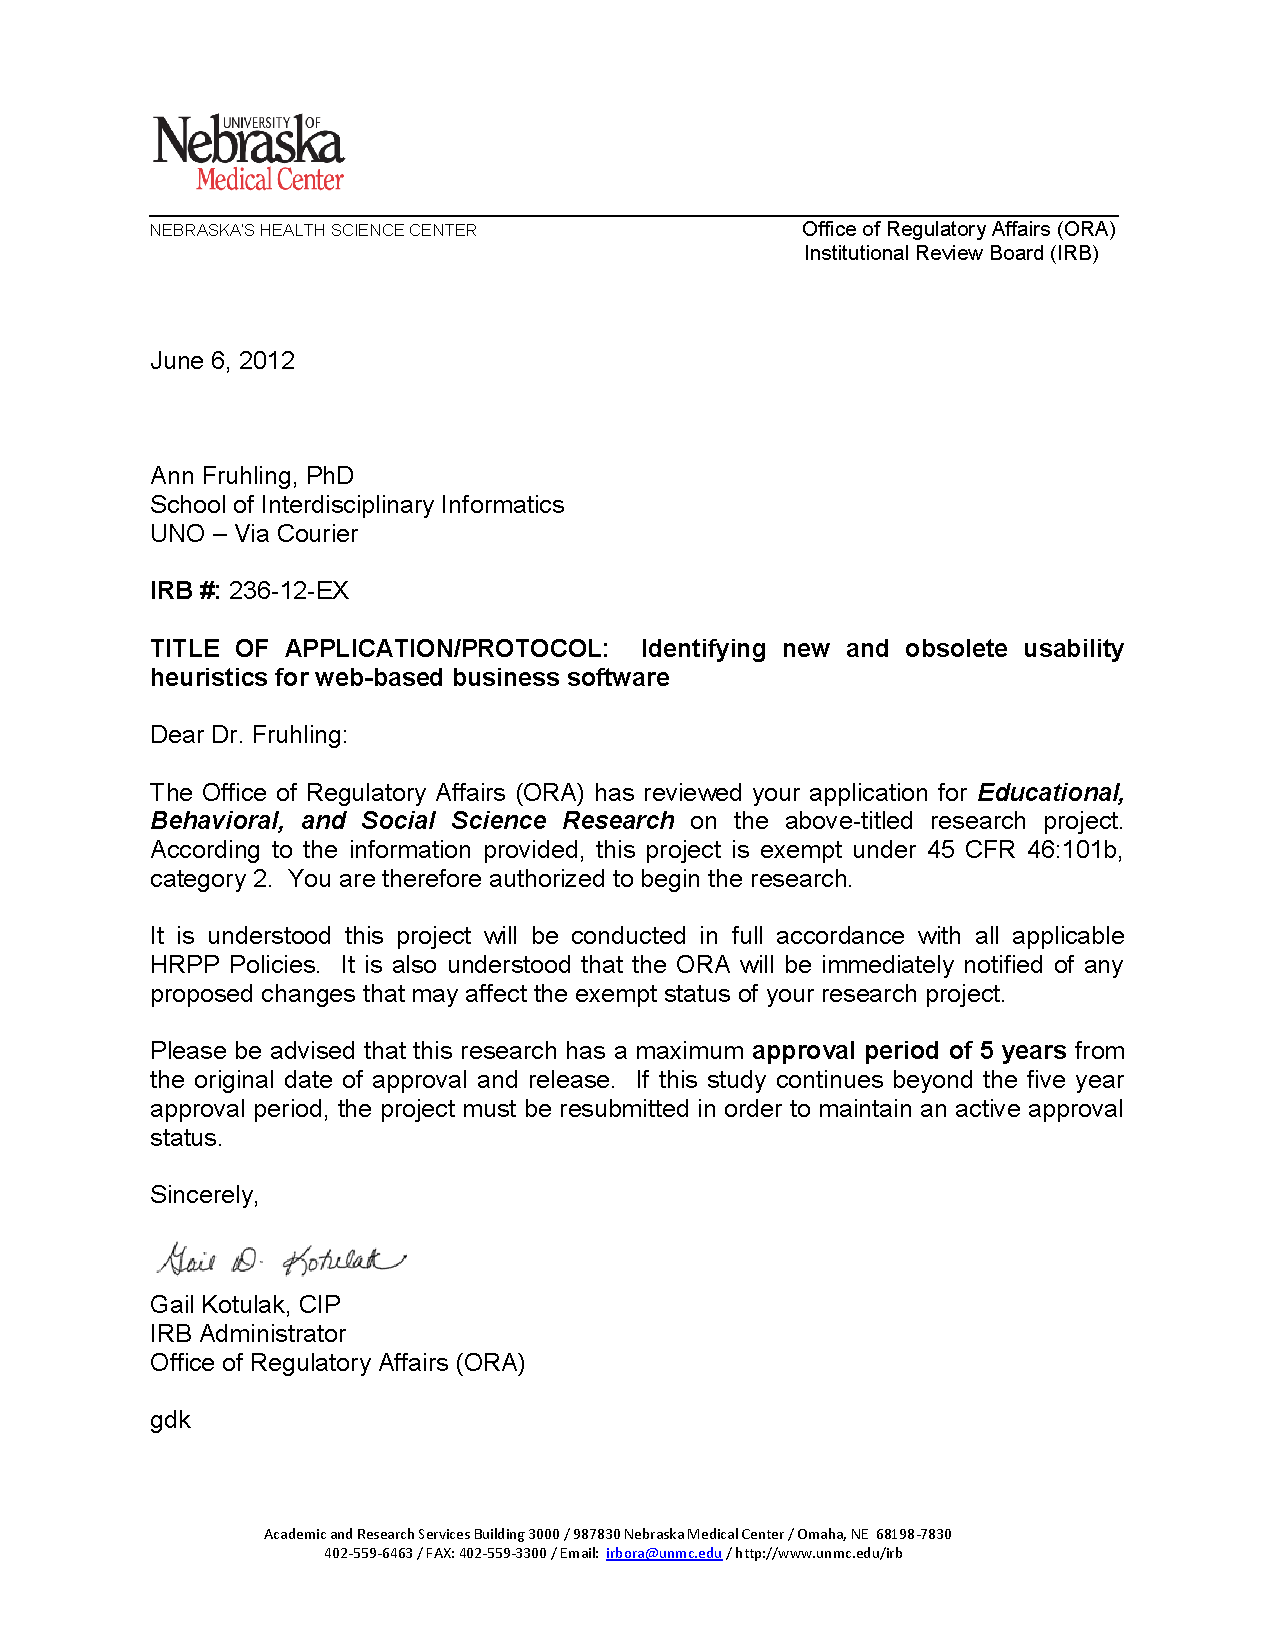
\includepdf[pages={1}]{irb_approval}

\section{Full Application}
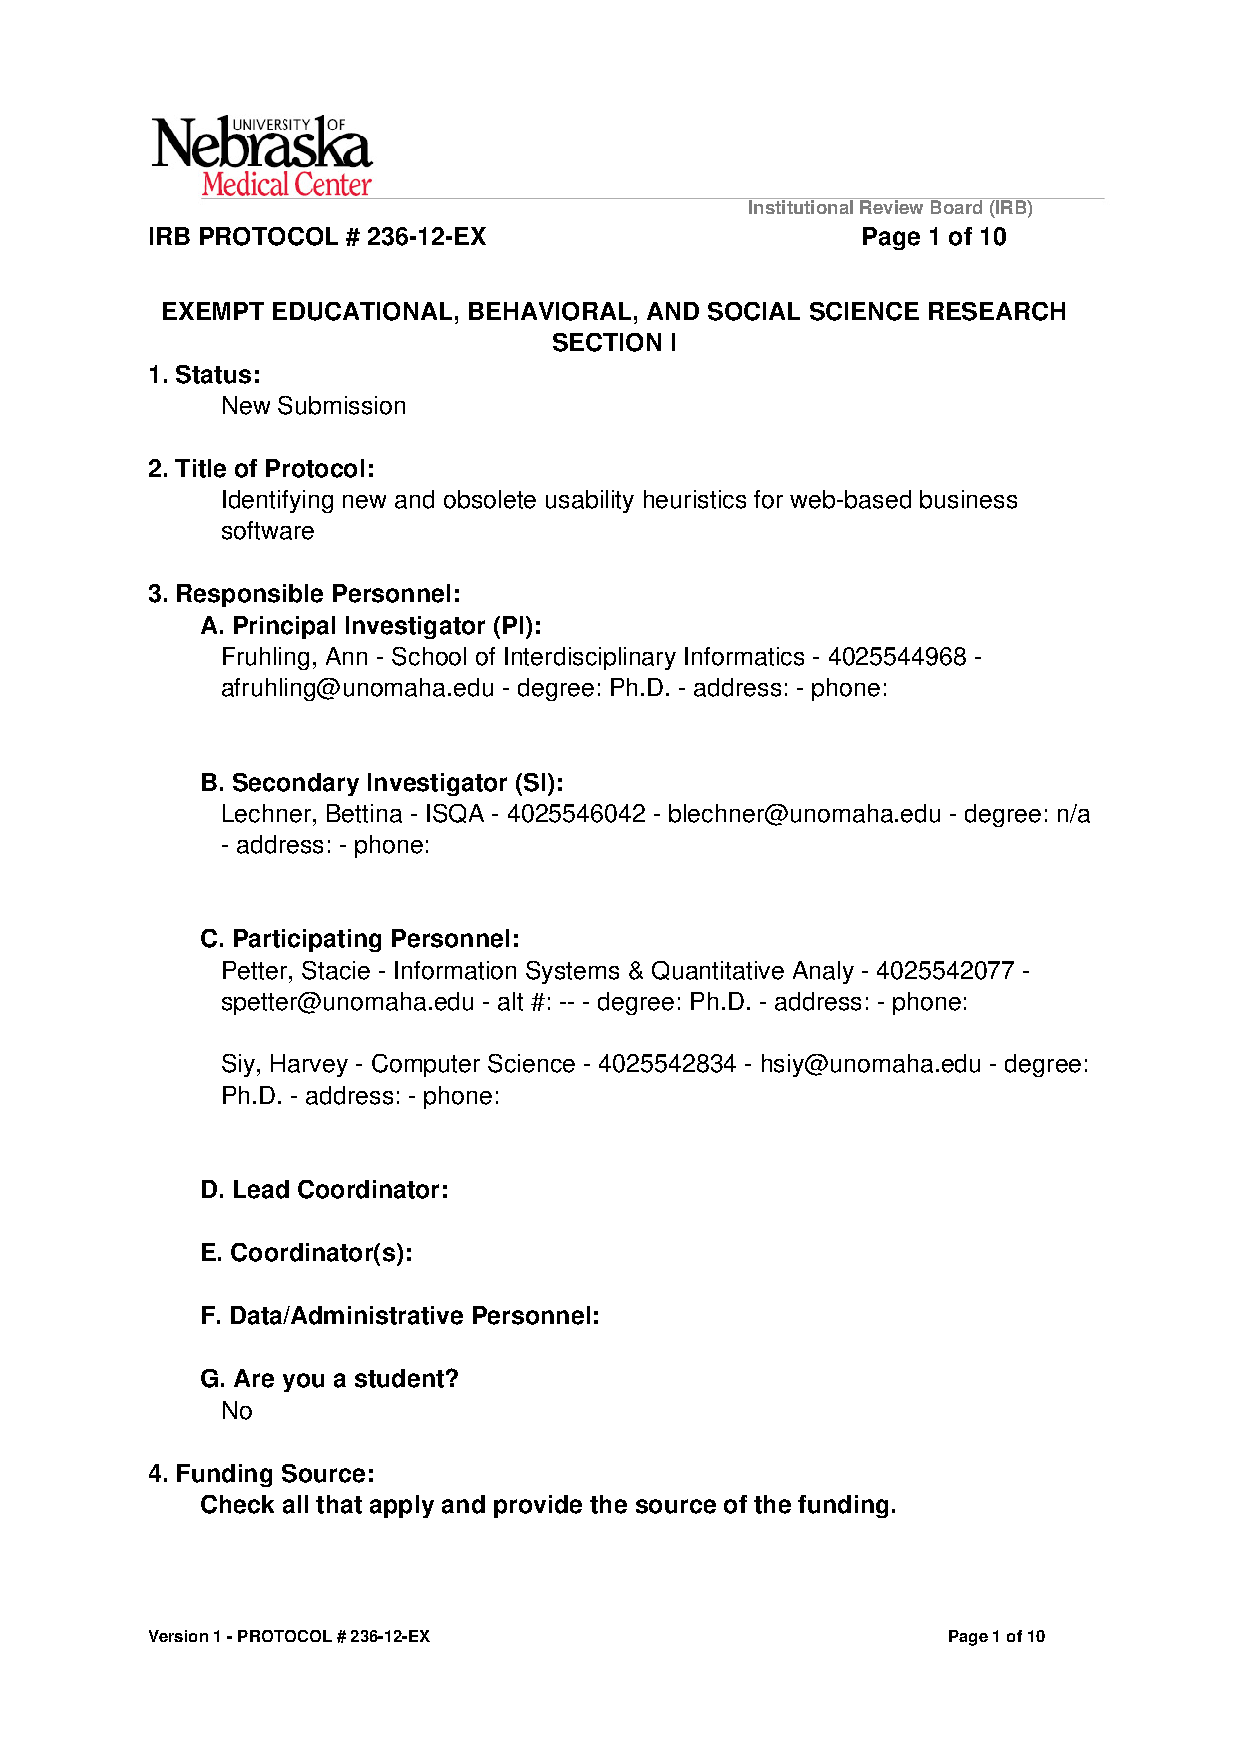
\includepdf[pages={1-10}]{irb}

\chapter{Materials Used in First Focus Group}
\label{app:first_group}
The following materials were used to provide context and information during the first focus group session, as well as before the session as pre-tasking material. Unless noted otherwise, the materials are provided in this chapter.

\begin{itemize}
	\item Description of CRM systems and functionality
	\item Screen shots of CRM systems (see appendix~\ref{app:screenshots})
	\item Existing heuristics identified in literature review (see appendix~\ref{appsec:litrev_list})
		\begin{itemize}
			\item Heuristics developed by \citet{Nielsen1994a}
			\item Heuristics for ERP systems developed by \citet{Singh2009}
			\item Heuristics for e-learning systems developed by \citet{Ardito2006}
		\end{itemize}
	\item Online live demo of Microsoft Dynamics CRM and salesforce.com
\end{itemize}

\section{Recruitment Material}
\input{./recruitment/expert}

\section{Background Questionnaire}
The following questions were used to collect information about the participants' experience in fields relevant to the study. The answers were collected through paper forms and were linked to the participants' responses throughout the study by assigning a unique ID number to each participant.

\tabulinesep=_2mm^2mm
\begin{longtabu} to \textwidth {X[1, p] r}		
	How many years of experience do you have working in the usability field? & \underline{\makebox[1in]{}}\\	
	How many years of experience do you have evaluating, designing, or developing user interfaces? & \underline{\makebox[1in]{}}\\
	How many years of experience do you have using a CRM system? & \underline{\makebox[1in]{}}\\	
	How many years of experience do you have evaluating, designing, or developing CRM systems? & \underline{\makebox[1in]{}}
\end{longtabu}

\section{Description of CRM Systems}
Customer relationship management (CRM) systems are used by many organizations to implement targeted marketing and advertising strategies and to build lucrative relationships with customers. To this end, these systems offer certain common functionalities \citep{Chaffey2011,Band2010b}:

\begin{itemize}
	\item Customer selection (identify types of customers to target, segment customers): customer business intelligence, customer data management
	\item Customer acquisition (perform marketing activities to form relationships with new customers): sales force automation (leads management, approval workflows, quoting), revenue and pricing management, order management
	\item Customer retention (perform marketing activities to maintain relationships with customers): electronic bill presentment and payment, interactive voice response, contact center infrastructure, customer service and support
	\item Customer extension (increase depth or range of products a customer purchases from the company): sales force automation, customer service management
\end{itemize}

\section{Instructions for Participants}
\subsection{Setup for Group Support System}
\begin{itemize}
\item URL: [removed]
\item User Name: [removed]
\item Session ID: [removed]
\item Session Passkey: [removed]
\end{itemize}

\subsection{Tasks}
\subsubsection*{Step 1}
Please review the informational materials about CRM systems on your desk. These materials include a short description of CRM systems and typical functionality and screen shots of two different web-based CRM systems. In addition, there should be a browser window open on your computer. The browser is logged into two web-based CRM systems (Microsoft Dynamics CRM and salesforce.com) you can interact with to familiarize yourself with their functionality.

\subsubsection*{Step 2}
Please review the list of heuristics on your desk. By design, some of these heuristics may be more applicable to web-based CRM systems than others. There may be some heuristics which seem like duplicates or are very similar to each other, but this is also intentional.

Log on to the group support system using the information provided above, where you will find the same list of usability heuristics. Please cast your vote with regard to how applicable you think each individual heuristic is to web-based CRM systems. You can also indicate whether you think any modifications to the original wording are necessary to account for CRM systems.

\subsubsection*{Step 3}
Once you are done voting, please proceed to the brainstorming activity. Please enter any heuristics that you think are relevant to web-based CRM systems, but are not present in the list you reviewed during the previous activity. As other participants enter their ideas, you can comment on them.

\subsubsection*{Step 4}
Participate in the group discussion led by the moderator.

\subsubsection*{Step 5}
Fill out the short questionnaire about your professional background.


\chapter{Materials Used in Second Focus Group}
\label{app:second_group}
The following materials were used for the second phase of the study which included CRM users.

\begin{itemize}
	\item Recruitment material
	\item List of usability heuristics developed by usability experts in first phase (see appendix section~\ref{appsec:experts_list})
	\item Background questionnaire
\end{itemize}

\section{Recruitment Material}
\input{./recruitment/user}

\section{Background Questionnaire}
The following questions were used to collect information about the participants' experience in fields relevant to the study. The answers were collected through paper forms and were linked to the participants' responses throughout the study by assigning a unique ID number to each participant.

\tabulinesep=_2mm^2mm
\begin{longtabu} to \textwidth {X[1, p] r}		
	How many years of experience do you have using a CRM (customer relationship management) system? & \underline{\makebox[1in]{}}\\	
	How many years of experience do you have using a web-based/ online CRM system (using an Internet browser such as Internet Explorer or Mozilla Firefox to access the system)? & \underline{\makebox[1in]{}} \\
	How often do you use the CRM system? & \underline{\makebox[1in]{}}
\end{longtabu}

\chapter{Lists of Heuristics Created}
This section contains the three lists developed in the various phases of this study. Section~\ref{appsec:litrev_list} consists of the heuristics selected in the literature review, which where presented to the usability experts for review. Section~\ref{appsec:experts_list} contains the heuristics developed by the usability experts during the first phase of the empirical study. This list was used as the basis for the second phase. Section~\ref{appsec:users_list} consists of the heuristics developed by the CRM users during the second phase of the empirical study. Please note that although each heuristic is linked back to its source in the tables following, the participants did not receive this information. They were only presented the heuristics themselves.

\section{List Based on Literature Review}
\label{appsec:litrev_list}

\begin{singlespace}
		\tabulinesep=_2mm^2mm
	\begin{longtabu} to \textwidth {X[1, p] c}
			\caption[List of heuristics developed during literature review]{List of heuristics developed during literature review; N = \citet{Nielsen1994a}, S = \citet{Singh2009}, A = \citet{Ardito2006}}\\
			\toprule
			\textbf{Heuristic} & \textbf{Source} \\
			\midrule
		\endfirsthead
			
			\textbf{Heuristic} & \textbf{Source} \\
			\midrule
		\endhead
		
			\bottomrule
		\endlastfoot
		
		The system should always keep users informed about what is going on, through appropriate feedback within reasonable time. & N \\
		The system should speak the users' language with words, phrases, and concepts familiar to the user, rather than system-oriented terms. Follow real-world conventions, making information appear in a natural and logical order. & N \\
		Users often choose system functions by mistake and will need a clearly marked "emergency exit" to leave the unwanted state without having to go through an extended dialogue. Support and undo and redo. & N \\
		Users should not have to wonder whether different words, situations, or actions mean the same thing. Follow platform conventions. & N \\
		Even better than good error messages is a careful design which prevents a problem from occurring in the first place. & N \\
		Make object, actions, and options visible. The user should not have to remember information from one part of the dialogue to another. Instructions for use of the system should be visible or easily retrievable whenever appropriate. & N \\
		Accelerators -- unseen by the novice user -- may often speed up the interaction for the expert user to such an extent that the system can cater to both inexperienced and experienced users. Allow users to tailor frequent actions. & N \\
		Dialogues should not contain information which is irrelevant or rarely needed. Every extra unit of information in a dialogue competes with the relevant units of information and diminishes their relative visibility. & N \\
		Error messages should be expressed in plain language (no codes), precisely indicate the problem, and constructively suggest a solution. & N \\
		Even though it is better if the system can be used without documentation, it may be necessary to provide help and documentation. Any such information should be easy to search, focused on the user's task, list concrete steps to be carried out, and not be too large. & N \\
		Information can be easily accessed & S \\
		Functionality can be found quickly and easily & S \\
		The system can guide the user through the correct sequence of transaction to complete a business process & S \\
		The UI supports efficient and accurate navigation of the system & S \\
		Functionality to search for information that is available & S \\
		There is a correlation between the searched item and the required information & S \\
		The system is capable of supporting the different interaction styles of the various users & S \\
		The system supports alternative navigation metaphors & S \\
		The system supports guidance-type information & S \\
		There is clarity in terms of the next sequence of transactions of steps & S \\
		The visual layout is well designed & S \\
		The information provided by the system is timely, accurate, complete and understandable & S \\
		The output is easy to understand and interpret, whether the output is structured & S \\
		The information presented supports informed decision making & S \\
		The output provided provides clear visibility into the various other departments & S \\
		The UI is intuitive & S \\
		Maintain UCD [user-centered design] attributes for interface graphical aspects & A \\
		Introduce mechanism to highlight errors and cues to avoid errors & A \\
		Provide the possibility to personalize interface graphics & A \\
		Clearly and constantly indicate system state & A \\
		Clearly visualize progress tracking & A \\
		Clearly visualize options and commands available & A \\
		Clearly visualize course structure & A \\
		Provide adaptation of the graphical aspect to the context of use & A \\
		The terminology used by the system is consistent with the terminology of the user & S \\
		The information provided by the system is in real-time & S \\
		The responses from the system are quick and efficient & S \\
		The system supports efficient completion of tasks & S \\
		The system improves user productivity & S \\
		The system automates routine and redundant tasks & S \\
		The system is easy to use & S \\
		The system supports improved information flow between the various organizational departments & S \\
		A user can learn how to use the system without a long introduction & S \\
		The various functions of the system can be identified by exploration & S \\
		There is sufficient on-line help to support the learning process & S \\
		It is easy to become skillful at using the system within a short amount of time & S \\
		The system is intimidating and complex to learn and use & S \\
		The ease in which the system can be configured to a particular industry type & S \\
		The capability of the system to support user-level customization & S \\
		The capability of the system to support customization for the user at a transaction level & S \\
		The alignment of the system to update existing business processes, and (or) to include new ones & S \\
		The ability of the system to be re-configured over a period of time & S \\
		The ability of the UI to be configured without affecting the underlying business logic of the system & S \\
		Provide support for the preparation of the multimedia material & A \\
		Highlight cross-references by state and course maps to facilitate topic links & A \\
		Supply different media channels for communication & A \\
		Maximize personalized access to learning contents & A \\
		Allow repository access to both lecturer and student & A \\
		Create contextualized bookmarks & A \\
		Enable off-line use of platform maintaining tools and learning context & A \\
		Insert assessment tests in various forms & A \\
		Automatically update students' progress tracking & A \\
		Insert learning domain tools & A \\
		Provide mechanisms to manage user's profiles & A \\
		Introduce mechanisms to prevent usage errors & A \\
		Provide mechanisms for teaching-through-errors & A \\
		Allow different repository modes for lecturers and students & A \\
		Insert easy to use platform tools & A \\
		Maximize adaptation of technology to the context of use & A \\
		Register the date of last modification of documents to facilitate updating & A \\
		Provide easy-to-use authoring tools & A \\
		Enable to define a clear learning path & A \\
		Allow to define alternative learning paths & A \\
		Provide support for assessment test & A \\
		Manage reports about attendance and usage of a course & A \\
		Allow use of learning tools even when not scheduled & A \\
		Provide both synchronous and asynchronous communication tools & A \\
		Provide communication mechanisms to both students and lecturers & A \\
		Allow the possibility to personalize the learning path & A \\
		Insert mechanisms to make annotations & A \\
		Provide mechanisms to integrate the didactic material & A \\
		Provide mechanisms for search by indexing, key or natural language & A \\
		Allow the possibility to create standard-compliant documents and tests (AICC, IMS, SCORM) & A \\
		Provide authoring tools to facilitate documents updating and assessment tests editing & A \\
	\end{longtabu}
\end{singlespace}

\section{List Developed by Usability Experts}
\label{appsec:experts_list}
\begin{singlespace}
		\tabulinesep=_2mm^2mm
	\begin{longtabu} to \textwidth {X[1, p] c}
			\caption[List of heuristics developed during first phase]{List of heuristics developed during first phase; * heuristic is a reworded version of original; N = \citet{Nielsen1994a}, S = \citet{Singh2009}, A = \citet{Ardito2006}}\\
			\toprule
			\textbf{Heuristic} & \textbf{Source} \\
			\midrule
		\endfirsthead
			
			\textbf{Heuristic} & \textbf{Source} \\
			\midrule
		\endhead
		
			\bottomrule
		\endlastfoot
		
		Maximize adaptation of technology to the context of use & A \\
		The system is customizable at the user level & A* \\
		Insert mechanisms to make annotations & A \\
		Clearly visualize user workflow & A* \\
		Clearly visualize options and commands available & A \\
		Clearly and constantly indicate system state & A \\
		Clearly visualize progress tracking & A \\
		Introduce mechanism to highlight errors and cues to avoid errors & A \\
		Provide mechanisms to manage user's profiles & A \\
		Provide mechanisms for search by indexing, key or natural language & A \\
		The system's communication mechanisms match the needs of the users & A* \\
		Maintain UCD [user-centered design] attributes for interface graphical aspects & A \\
		Highlight cross-references between different types of data (e.g. customer issues, sales support, and marketing campaigns) & A* \\
		Register the date of last modification of documents to facilitate updating & A \\
		Provide easy-to-use authoring tools & A \\
		Supply different media channels for communication & A \\
		Introduce mechanisms to prevent usage errors & A \\
		Provide both synchronous and asynchronous communication tools & A \\
		The system conforms to platform conventions & A* \\
		Provide mechanisms for teaching-through-errors & A \\
		Clearly visualize employee performace & A* \\
		Even better than good error messages is a careful design which prevents a problem from occurring in the first place. & N \\
		Error messages should be expressed in plain language (no codes), precisely indicate the problem, and constructively suggest a solution. & N \\
		Even though it is better if the system can be used without documentation, it may be necessary to provide help and documentation. Any such information should be easy to search, focused on the user's task, list concrete steps to be carried out, and not be too large. & N \\
		Dialogues should not contain information which is irrelevant or rarely needed. Every extra unit of information in a dialogue competes with the relevant units of information and diminishes their relative visibility. & N \\
		Accelerators -- unseen by the novice user -- may often speed up the interaction for the expert user to such an extent that the system can cater to both inexperienced and experienced users. Allow users to tailor frequent actions. & N \\
		Make object, actions, and options visible. The user should not have to remember information from one part of the dialogue to another. Instructions for use of the system should be visible or easily retrievable whenever appropriate. & N \\
		Users should not have to wonder whether different words, situations, or actions mean the same thing. Follow platform conventions. & N \\
		The system should always keep users informed about what is going on, through appropriate feedback within reasonable time. & N \\
		The system should speak the users' language with words, phrases, and concepts familiar to the user, rather than system-oriented terms. Follow real-world conventions, making information appear in a natural and logical order. & N \\
		Users often choose system functions by mistake and will need a clearly marked "emergency exit" to leave the unwanted state without having to go through an extended dialogue. Support and undo and redo. & N \\
		The system provides appropriate filters to organize data & New \\
		The system has a dashboard which provides a quick glance of the current status & New \\
		The system displays appropriate information depending on the task at hand & New \\
		Help and documentation are immersed in the system, non-obtrusive, and ubiquitous & New \\
		The system allows for tailoring of the interface to an individual's workflow & New \\
		The terminology used by the system is consistent with the terminology of the user & S \\
		The various functions of the system can be identified by exploration & S \\
		The system is capable of supporting the different interaction styles of the various users & S \\
		Functionality can be found quickly and easily & S \\
		The information provided by the system is in real-time & S \\
		The ability of the system to be re-configured over a period of time & S \\
		The output style fits the type of data being displayed & S* \\
		The responses from the system are quick and efficient & S \\
		The system is easy to use & S \\
		The ease in which the system can be configured to a particular industry type & S \\
		The system supports efficient completion of tasks & S \\
		The system can guide the user through the correct sequence of transaction to complete a business process & S \\
		The system reduces intimidation and complexity by providing positive feedback and reinforcement, a clear path to execution, and a terminology that matches the users' language & S* \\
		The output provided provides clear visibility into the various other departments & S \\
		The capability of the system to support user-level customization & S \\
		The system automates routine and redundant tasks & S \\
		The alignment of the system to update existing business processes, and (or) to include new ones & S \\
		The results returned by a search are relevant to the information required by the user & S* \\
		The ability of the UI to be configured without affecting the underlying business logic of the system & S \\
		Information can be easily accessed & S \\
		The system supports improved information flow between the various organizational departments & S \\
		There is clarity in terms of the next sequence of transactions of steps & S \\
		It is easy to become skillful at using the system within a short amount of time & S \\
		The UI supports efficient and accurate navigation of the system & S \\
		The system improves user productivity & S \\
		Functionality to search for information that is available & S \\
		The information provided by the system is timely, accurate, complete and understandable & S \\
		The information presented supports informed decision making & S \\
		There is sufficient on-line help to support the learning process & S \\
		The visual layout is well designed & S \\
		The UI is intuitive & S \\
		A user can learn how to use the system without a long introduction & S \\
	\end{longtabu}
\end{singlespace}

\section{List Validated by CRM Users}
\label{appsec:users_list}
\begin{singlespace}
		\tabulinesep=_2mm^2mm
	\begin{longtabu} to \textwidth {X[1, p] c}
			\caption[List of heuristics developed during second phase]{List of heuristics developed during second phase; * heuristic is a reworded version of original; N = \citet{Nielsen1994a}, S = \citet{Singh2009}, A = \citet{Ardito2006}, New = newly developed heuristic}\\
			\toprule
			\textbf{Heuristic} & \textbf{Source} \\
			\midrule
		\endfirsthead
			
			\textbf{Heuristic} & \textbf{Source} \\
			\midrule
		\endhead
		
			\bottomrule
		\endlastfoot
		
		Clearly and constantly indicate system state & A \\
		Clearly visualize employee performance & A* \\
		Clearly visualize options and commands available & A \\
		Clearly visualize progress tracking & A \\
		Clearly visualize user workflow & A* \\
		Highlight cross-references between different types of data (e.g. customer issues, sales support, and marketing campaigns) & A* \\
		Insert mechanisms to make annotations & A \\
		Introduce mechanism to highlight errors and cues to avoid errors & A \\
		Introduce mechanisms to prevent usage errors & A \\
		Maintain UCD [user-centered design] attributes for interface graphical aspects & A \\
		Maximize adaptation of technology to the context of use & A \\
		Provide both synchronous and asynchronous communication tools & A \\
		Provide easy-to-use authoring tools & A \\
		Provide mechanisms for search by indexing, key or natural language & A \\
		Provide mechanisms for teaching-through-errors & A \\
		Provide mechanisms to manage user's profiles & A \\
		Register the date of last modification of documents to facilitate updating & A \\
		Supply different media channels for communication & A \\
		The system conforms to platform conventions & A* \\
		The system is customizable at the user level & A* \\
		The system's communication mechanisms match the needs of the users & A* \\
		Accelerators -- unseen by the novice user -- may often speed up the interaction for the expert user to such an extent that the system can cater to both inexperienced and experienced users. Allow users to tailor frequent actions. & N \\
		Dialogues should not contain information which is irrelevant or rarely needed. Every extra unit of information in a dialogue competes with the relevant units of information and diminishes their relative visibility. & N \\
		Error messages should be expressed in plain language (no codes), precisely indicate the problem, and constructively suggest a solution. & N \\
		Even better than good error messages is a careful design which prevents a problem from occurring in the first place. & N \\
		Even though it is better if the system can be used without documentation, it may be necessary to provide help and documentation. Any such information should be easy to search, focused on the user's task, list concrete steps to be carried out, and not be too large. & N \\
		Make object, actions, and options visible. The user should not have to remember information from one part of the dialogue to another. Instructions for use of the system should be visible or easily retrievable whenever appropriate. & N \\
		The system should always keep users informed about what is going on, through appropriate feedback within reasonable time. & N \\
		The system should speak the users' language with words, phrases, and concepts familiar to the user, rather than system-oriented terms. Follow real-world conventions, making information appear in a natural and logical order. & N \\
		Users should not have to wonder whether different words, situations, or actions mean the same thing. Follow platform conventions. & N \\
		Help and documentation are immersed in the system, non-obtrusive, and ubiquitous & New \\
		The system allows for tailoring of the interface to an individual's workflow & New \\
		The system displays appropriate information depending on the task at hand & New \\
		The system has a dashboard which provides a quick glance of the current status & New \\
		The system provides appropriate filters to organize data & New \\
		A user can learn how to use the system without a long introduction & S \\
		Functionality can be found quickly and easily & S \\
		Functionality to search for information that is available & S \\
		Information can be easily accessed & S \\
		It is easy to become skillful at using the system within a short amount of time & S \\
		The ability of the system to be re-configured over a period of time & S \\
		The ability of the UI to be configured without affecting the underlying business logic of the system & S \\
		The alignment of the system to update existing business processes, and (or) to include new ones & S \\
		The capability of the system to support user-level customization & S \\
		The ease in which the system can be configured to a particular industry type & S \\
		The information presented supports informed decision making & S \\
		The information provided by the system is in real-time & S \\
		The information provided by the system is timely, accurate, complete and understandable & S \\
		The output provided provides clear visibility into the various other departments & S \\
		The output style fits the type of data being displayed & S* \\
		The responses from the system are quick and efficient & S \\
		The results returned by a search are relevant to the information required by the user & S* \\
		The system automates routine and redundant tasks & S \\
		The system can guide the user through the correct sequence of transaction to complete a business process & S \\
		The system improves user productivity & S \\
		The system is capable of supporting the different interaction styles of the various users & S \\
		The system is easy to use & S \\
		The system reduces intimidation and complexity by providing positive feedback and reinforcement, a clear path to execution, and a terminology that matches the users' language & S* \\
		The system supports efficient completion of tasks & S \\
		The system supports improved information flow between the various organizational departments & S \\
		The terminology used by the system is consistent with the terminology of the user & S \\
		The UI [user interface] is intuitive & S \\
		The UI supports efficient and accurate navigation of the system & S \\
		The various functions of the system can be identified by exploration & S \\
		The visual layout is well designed & S \\
		There is clarity in terms of the next sequence of transactions of steps & S \\
		There is sufficient on-line help to support the learning process & S \\
	\end{longtabu}
\end{singlespace}

\section{Final, Unified List of Heuristics}
\label{appsec:final}
\begin{singlespace}
		\tabulinesep=_1mm^1mm
	\begin{longtabu} to \textwidth {l X[1, p] c}
			\caption{Final, unified list of heuristics for web-based CRM systems}\\
			\toprule
			\textbf{Category} & \textbf{Heuristic} & \textbf{Source} \\
			\midrule
		\endfirsthead
			
			\textbf{Category} & \textbf{Heuristic} & \textbf{Source} \\
			\midrule
		\endhead
		
			\bottomrule
		\endlastfoot
		
		Application Proactivity & Introduce mechanisms to prevent usage errors & A \\
		Application Proactivity & Maximize adaptation of technology to the context of use & A \\
		Application Proactivity & Provide mechanisms for teaching-through-er\-rors & A \\
		Application Proactivity & Provide mechanisms to manage user's profiles & A \\
		Application Proactivity & Register the date of last modification of documents to facilitate updating & A \\
		Application Proactivity & The system conforms to platform conventions & A \\
		Customization & The ability of the system to be re-configured over a period of time & S \\
		Customization & The ability of the UI to be configured without affecting the underlying business logic of the system & S \\
		Customization & The alignment of the system to update existing business processes, and (or) to include new ones & S \\
		Customization & The capability of the system to support user-level customization & S \\
		Customization & The ease in which the system can be configured to a particular industry type & S \\
		Customization & The system allows for tailoring of the interface to an individual's workflow & New \\
		Learnability & A user can learn how to use the system without a long introduction & S \\
		Learnability & Even though it is better if the system can be used without documentation, it may be necessary to provide help and documentation. Any such information should be easy to search, focused on the user's task, list concrete steps to be carried out, and not be too large. & N \\
		Learnability & Help and documentation are immersed in the system, non-obtrusive, and ubiquitous & New \\
		Learnability & It is easy to become skillful at using the system within a short amount of time & S \\
		Learnability & The system reduces intimidation and complexity by providing positive feedback and reinforcement, a clear path to execution, and a terminology that matches the users' language & S \\
		Learnability & The various functions of the system can be identified by exploration & S \\
		Learnability & There is sufficient on-line help to support the learning process & S \\
		Navigation & Accelerators -- unseen by the novice user -- may often speed up the interaction for the expert user to such an extent that the system can cater to both inexperienced and experienced users. Allow users to tailor frequent actions. & N \\
		Navigation & Even better than good error messages is a careful design which prevents a problem from occurring in the first place. & N \\
		Navigation & Functionality can be found quickly and easily & S \\
		Navigation & Functionality to search for information that is available & S \\
		Navigation & Information can be easily accessed & S \\
		Navigation & Make object, actions, and options visible. The user should not have to remember information from one part of the dialogue to another. Instructions for use of the system should be visible or easily retrievable whenever appropriate. & N \\
		Navigation & The results returned by a search are relevant to the information required by the user & S \\
		Navigation & The system can guide the user through the correct sequence of transaction to complete a business process & S \\
		Navigation & The system is capable of supporting the different interaction styles of the various users & S \\
		Navigation & The UI supports efficient and accurate navigation of the system & S \\
		Navigation & There is clarity in terms of the next sequence of transactions of steps & S \\
		Presentation & Clearly and constantly indicate system state & A \\
		Presentation & Clearly visualize employee performance & A \\
		Presentation & Clearly visualize options and commands available & A \\
		Presentation & Clearly visualize progress tracking & A \\
		Presentation & Clearly visualize user workflow & A \\
		Presentation & Dialogues should not contain information wh\-ich is irrelevant or rarely needed. Every extra unit of information in a dialogue competes with the relevant units of information and diminishes their relative visibility. & N \\
		Presentation & Error messages should be expressed in plain language (no codes), precisely indicate the problem, and constructively suggest a solution. & N \\
		Presentation & Introduce mechanism to highlight errors and cues to avoid errors & A \\
		Presentation & Maintain UCD [user-centered design] at\-trib\-utes for interface graphical aspects & A \\
		Presentation & The information presented supports informed decision making & S \\
		Presentation & The information provided by the system is timely, accurate, complete and understandable & S \\
		Presentation & The output provided provides clear visibility into the various other departments & S \\
		Presentation & The output style fits the type of data being displayed & S \\
		Presentation & The system is accessible and usable from mobile devices & New \\
		Presentation & The system is customizable at the user level & A \\
		Presentation & The system should always keep users informed about what is going on, through appropriate feedback within reasonable time. & N \\
		Presentation & The UI [user interface] is intuitive & S \\
		Presentation & The visual layout is well designed & S \\
		Task Support & Highlight cross-references between different ty\-pes of data (e.g. customer issues, sales support, and marketing campaigns) & A \\
		Task Support & Supply different media channels for communication & A \\
		Task Support & The information provided by the system is in real-time & S \\
		Task Support & The responses from the system are quick and efficient & S \\
		Task Support & The system allows for synchronization of its information with outside communication tools & New \\
		Task Support & The system automates routine and redundant tasks & S \\
		Task Support & The system displays appropriate information depending on the task at hand & New \\
		Task Support & The system has a dashboard which provides a quick glance of the current status & New \\
		Task Support & The system improves user productivity & S \\
		Task Support & The system is easy to use & S \\
		Task Support & The system provides appropriate filters to organize data & New \\
		Task Support & The system should speak the users' language with words, phrases, and concepts familiar to the user, rather than system-oriented terms. Follow real-world conventions, making information appear in a natural and logical order. & N \\
		Task Support & The system supports efficient completion of tasks & S \\
		Task Support & The system supports improved information flow between the various organizational departments & S \\
		Task Support & The terminology used by the system is consistent with the terminology of the user & S \\
		Task Support & Users often choose system functions by mistake and will need a clearly marked "emergency exit" to leave the unwanted state without having to go through an extended dialogue. Support and undo and redo. & N \\
		Task Support & Users should not have to wonder whether different words, situations, or actions mean the same thing. Follow platform conventions. & N \\
		User Activity & Insert mechanisms to make annotations & A \\
		User Activity & Provide both synchronous and asynchronous communication tools & A \\
		User Activity & Provide easy-to-use authoring tools & A \\
		User Activity & Provide mechanisms for search by indexing, key or natural language & A \\
		User Activity & The system's communication mechanisms mat\-ch the needs of the users & A \\
	\end{longtabu}
\end{singlespace}

\chapter{Detailed Results}
\label{app:results}

\section{First Phase}
\label{appsec:results_first}
\begin{landscape}
\begin{singlespace}
		\tabulinesep=_2mm^2mm
\begin{longtabu} to 650pt {X[6, p] X[1, p] X[1, p] X[1, p] X[1, p]}
			\caption{Mean and standard deviation for each heuristic's rating of applicability to CRM systems and need for rewording}\\
			\toprule
			& \multicolumn2{c}{\textbf{Applicability}} & \multicolumn2{c}{\textbf{Need for Rewording}} \\
			\textbf{Heuristic} & \textbf{Mean} & \textbf{Std.\ Dev.} & \textbf{Mean} & \textbf{Std.\ Dev.} \\
			\midrule
		\endfirsthead
		
			& \multicolumn2{c}{\textbf{Applicability}} & \multicolumn2{c}{\textbf{Need for Rewording}} \\
			\textbf{Heuristic} & \textbf{Mean} & \textbf{Std.\ Dev.} & \textbf{Mean} & \textbf{Std.\ Dev.} \\
			\midrule
		\endhead
		
			\bottomrule
		\endlastfoot
		
		The system should always keep users informed about what is going on, through appropriate feedback within reasonable time. & 3.8 & 0.837 & 0.0 & 0.000 \\
The system should speak the users' language with words, phrases, and concepts familiar to the user, rather than system-oriented terms. Follow real-world conventions, making information appear in a natural and logical order. & 4.0 & 0.707 & 0.0 & 0.000 \\
Users often choose system functions by mistake and will need a clearly marked "emergency exit" to leave the unwanted state without having to go through an extended dialogue. Support and undo and redo. & 4.6 & 0.894 & 0.0 & 0.000 \\
Users should not have to wonder whether different words, situations, or actions mean the same thing. Follow platform conventions. & 4.4 & 0.894 & 0.0 & 0.000 \\
Even better than good error messages is a careful design which prevents a problem from occurring in the first place. & 4.0 & 1.000 & 0.0 & 0.000 \\
Make object, actions, and options visible. The user should not have to remember information from one part of the dialogue to another. Instructions for use of the system should be visible or easily retrievable whenever appropriate. & 4.0 & 0.707 & 0.0 & 0.000 \\
Accelerators---unseen by the novice user---may often speed up the interaction for the expert user to such an extent that the system can cater to both inexperienced and experienced users. Allow users to tailor frequent actions. & 4.4 & 0.894 & 0.0 & 0.000 \\
Dialogues should not contain information which is irrelevant or rarely needed. Every extra unit of information in a dialogue competes with the relevant units of information and diminishes their relative visibility. & 3.8 & 0.837 & 0.4 & 0.548 \\
Error messages should be expressed in plain language (no codes), precisely indicate the problem, and constructively suggest a solution. & 4.0 & 0.707 & 0.0 & 0.000 \\
Even though it is better if the system can be used without documentation, it may be necessary to provide help and documentation. Any such information should be easy to search, focused on the user's task, list concrete steps to be carried out, and not be too large. & 4.0 & 0.707 & 0.0 & 0.000 \\
Information can be easily accessed & 4.0 & 1.000 & 0.4 & 0.548 \\
Functionality can be found quickly and easily & 3.8 & 0.447 & 0.2 & 0.447 \\
The system can guide the user through the correct sequence of transaction to complete a business process & 4.0 & 1.225 & 0.2 & 0.447 \\
The UI supports efficient and accurate navigation of the system & 4.2 & 0.837 & 0.2 & 0.447 \\
Functionality to search for information that is available & 3.4 & 1.140 & 0.6 & 0.548 \\
There is a correlation between the searched item and the required information & 3.4 & 1.140 & 0.6 & 0.548 \\
The system is capable of supporting the different interaction styles of the various users & 3.8 & 1.304 & 0.0 & 0.000 \\
The system supports alternative navigation metaphors & 2.8 & 1.304 & 0.4 & 0.548 \\
The system supports guidance-type information & 2.8 & 0.837 & 0.8 & 0.447 \\
There is clarity in terms of the next sequence of transactions of steps & 3.8 & 1.304 & 0.2 & 0.447 \\
The visual layout is well designed & 4.0 & 0.707 & 0.6 & 0.548 \\
The information provided by the system is timely, accurate, complete and understandable & 4.4 & 0.894 & 0.4 & 0.548 \\
The output is easy to understand and interpret, whether the output is structured & 3.6 & 0.548 & 0.8 & 0.447 \\
The information presented supports informed decision making & 4.2 & 0.837 & 0.2 & 0.447 \\
The output provided provides clear visibility into the various other departments & 3.0 & 1.414 & 0.4 & 0.548 \\
The UI is intuitive & 3.8 & 0.447 & 0.4 & 0.548 \\
Maintain UCD [user-centered design] attributes for interface graphical aspects & 4.0 & 0.707 & 0.4 & 0.548 \\
Introduce mechanism to highlight errors and cues to avoid errors & 3.8 & 0.837 & 0.0 & 0.000 \\
Provide the possibility to personalize interface graphics & 2.8 & 1.483 & 0.0 & 0.000 \\
Clearly and constantly indicate system state & 3.8 & 0.837 & 0.0 & 0.000 \\
Clearly visualize progress tracking & 3.2 & 1.304 & 0.2 & 0.447 \\
Clearly visualize options and commands available & 3.8 & 0.447 & 0.2 & 0.447 \\
Clearly visualize course structure & 2.0 & 0.707 & 0.8 & 0.447 \\
Provide adaptation of the graphical aspect to the context of use & 2.4 & 0.548 & 0.8 & 0.447 \\
The terminology used by the system is consistent with the terminology of the user & 4.6 & 0.548 & 0.0 & 0.000 \\
The information provided by the system is in real-time & 3.8 & 1.304 & 0.2 & 0.447 \\
The responses from the system are quick and efficient & 4.0 & 0.707 & 0.0 & 0.000 \\
The system supports efficient completion of tasks & 4.0 & 1.225 & 0.0 & 0.000 \\
The system improves user productivity & 3.6 & 1.140 & 0.4 & 0.548 \\
The system automates routine and redundant tasks & 4.2 & 0.837 & 0.0 & 0.000 \\
The system is easy to use & 3.8 & 0.837 & 0.4 & 0.548 \\
The system supports improved information flow between the various organizational departments & 3.8 & 1.304 & 0.0 & 0.000 \\
A user can learn how to use the system without a long introduction & 4.0 & 0.707 & 0.0 & 0.000 \\
The various functions of the system can be identified by exploration & 3.8 & 0.447 & 0.0 & 0.000 \\
There is sufficient on-line help to support the learning process & 3.8 & 0.837 & 0.0 & 0.000 \\
It is easy to become skillful at using the system within a short amount of time & 3.4 & 0.548 & 0.4 & 0.548 \\
The system is intimidating and complex to learn and use & 1.4 & 0.894 & 0.6 & 0.548 \\
The ease in which the system can be configured to a particular industry type & 4.0 & 0.000 & 0.2 & 0.447 \\
The capability of the system to support user-level customization & 3.4 & 1.140 & 0.0 & 0.000 \\
The capability of the system to support customization for the user at a transaction level & 2.8 & 0.837 & 0.0 & 0.000 \\
The alignment of the system to update existing business processes, and (or) to include new ones & 4.2 & 0.447 & 0.0 & 0.000 \\
The ability of the system to be re-configured over a period of time & 3.8 & 1.095 & 0.0 & 0.000 \\
The ability of the UI to be configured without affecting the underlying business logic of the system & 4.4 & 0.548 & 0.0 & 0.000 \\
Provide support for the preparation of the multimedia material & 2.6 & 1.342 & 0.2 & 0.447 \\
Highlight cross-references by state and course maps to facilitate topic links & 2.2 & 0.837 & 0.6 & 0.548 \\
Supply different media channels for communication & 3.6 & 0.894 & 0.2 & 0.447 \\
Maximize personalized access to learning contents & 2.8 & 0.447 & 0.4 & 0.548 \\
Allow repository access to both lecturer and student & 2.0 & 1.732 & 0.4 & 0.548 \\
Create contextualized bookmarks & 2.8 & 1.643 & 0.4 & 0.548 \\
Enable off-line use of platform maintaining tools and learning context & 2.8 & 1.304 & 0.4 & 0.548 \\
Insert assessment tests in various forms & 1.4 & 0.548 & 0.0 & 0.000 \\
Automatically update students' progress tracking & 1.6 & 0.548 & 0.4 & 0.548 \\
Insert learning domain tools & 1.8 & 0.837 & 0.4 & 0.548 \\
Provide mechanisms to manage user's profiles & 3.2 & 0.837 & 0.2 & 0.447 \\
Introduce mechanisms to prevent usage errors & 3.8 & 0.447 & 0.0 & 0.000 \\
Provide mechanisms for teaching-through-errors & 3.2 & 1.304 & 0.0 & 0.000 \\
Allow different repository modes for lecturers and students & 1.8 & 1.304 & 0.8 & 0.447 \\
Insert easy to use platform tools & 2.0 & 0.707 & 0.6 & 0.548 \\
Maximize adaptation of technology to the context of use & 3.0 & 1.000 & 0.4 & 0.548 \\
Register the date of last modification of documents to facilitate updating & 4.6 & 0.548 & 0.0 & 0.000 \\
Provide easy-to-use authoring tools & 3.6 & 1.140 & 0.2 & 0.447 \\
Enable to define a clear learning path & 2.2 & 0.837 & 0.4 & 0.548 \\
Allow to define alternative learning paths & 2.2 & 0.837 & 0.4 & 0.548 \\
Provide support for assessment test & 2.0 & 0.707 & 0.2 & 0.447 \\
Manage reports about attendance and usage of a course & 1.8 & 0.837 & 0.2 & 0.447 \\
Allow use of learning tools even when not scheduled & 2.2 & 1.095 & 0.2 & 0.447 \\
Provide both synchronous and asynchronous communication tools & 3.6 & 0.548 & 0.0 & 0.000 \\
Provide communication mechanisms to both students and lecturers & 2.0 & 0.707 & 0.6 & 0.548 \\
Allow the possibility to personalize the learning path & 2.0 & 0.707 & 0.4 & 0.548 \\
Insert mechanisms to make annotations & 3.6 & 1.517 & 0.2 & 0.447 \\
Provide mechanisms to integrate the didactic material & 1.8 & 0.447 & 0.6 & 0.548 \\
Provide mechanisms for search by indexing, key or natural language & 3.6 & 1.140 & 0.2 & 0.447 \\
Allow the possibility to create standard-compliant documents and tests (AICC, IMS, SCORM) & 1.6 & 0.548 & 0.2 & 0.447 \\
Provide authoring tools to facilitate documents updating and assessment tests editing & 2.4 & 1.140 & 0.2 & 0.447 \\
\end{longtabu}
\end{singlespace}
\end{landscape}

\section{Second Phase}
\label{appsec:results_second}
\begin{landscape}
\begin{singlespace}
		\tabulinesep=_2mm^2mm
\begin{longtabu} to 650pt {X[7, p] X[1, p] X[1, p]}
			\caption{Mean and standard deviation for each heuristic's rating of applicability to CRM systems}\\
			\toprule
			& \multicolumn2{c}{\textbf{Applicability}} \\
			\textbf{Heuristic} & \textbf{Mean} & \textbf{Std.\ Dev.} \\
			\midrule
		\endfirsthead
		
			& \multicolumn2{c}{\textbf{Applicability}}  \\
			\textbf{Heuristic} & \textbf{Mean} & \textbf{Std.\ Dev.} \\
			\midrule
		\endhead
		
			\bottomrule
		\endlastfoot
		
		Clearly and constantly indicate system state & 3.80 & 1.166 \\
		Clearly visualize employee performance & 4.83 & 0.373 \\
		Clearly visualize options and commands available & 4.00 & 1.000 \\
		Clearly visualize progress tracking & 4.60 & 0.490 \\
		Clearly visualize user workflow & 4.33 & 0.943 \\
		Highlight cross-references between different types of data (e.g. customer issues, sales support, and marketing campaigns) & 4.83 & 0.373 \\
		Insert mechanisms to make annotations & 3.40 & 0.490 \\
		Introduce mechanism to highlight errors and cues to avoid errors & 3.00 & 0.632 \\
		Introduce mechanisms to prevent usage errors & 4.60 & 0.490 \\
		Maintain UCD [user-centered design] attributes for interface graphical aspects & 4.25 & 0.829 \\
		Maximize adaptation of technology to the context of use & 4.33 & 0.471 \\
		Provide both synchronous and asynchronous communication tools & 4.50 & 0.500 \\
		Provide easy-to-use authoring tools & 3.75 & 1.299 \\
		Provide mechanisms for search by indexing, key or natural language & 4.20 & 1.166 \\
		Provide mechanisms for teaching-through-errors & 3.00 & 1.265 \\
		Provide mechanisms to manage user's profiles & 3.20 & 1.166 \\
		Register the date of last modification of documents to facilitate updating & 4.60 & 0.490 \\
		Supply different media channels for communication & 4.00 & 1.414 \\
		The system conforms to platform conventions & 3.67 & 0.943 \\
		The system is customizable at the user level & 3.50 & 1.258 \\
		The system's communication mechanisms match the needs of the users & 4.17 & 1.067 \\
		Accelerators -- unseen by the novice user -- may often speed up the interaction for the expert user to such an extent that the system can cater to both inexperienced and experienced users. Allow users to tailor frequent actions. & 3.60 & 1.020 \\
		Dialogues should not contain information which is irrelevant or rarely needed. Every extra unit of information in a dialogue competes with the relevant units of information and diminishes their relative visibility. & 3.00 & 1.414 \\
		Error messages should be expressed in plain language (no codes), precisely indicate the problem, and constructively suggest a solution. & 5.00 & 0.000 \\
		Even better than good error messages is a careful design which prevents a problem from occurring in the first place. & 4.33 & 0.471 \\
		Even though it is better if the system can be used without documentation, it may be necessary to provide help and documentation. Any such information should be easy to search, focused on the user's task, list concrete steps to be carried out, and not be too large. & 4.33 & 0.471 \\
		Make object, actions, and options visible. The user should not have to remember information from one part of the dialogue to another. Instructions for use of the system should be visible or easily retrievable whenever appropriate. & 4.67 & 0.471 \\
		The system should always keep users informed about what is going on, through appropriate feedback within reasonable time. & 4.40 & 0.800 \\
		The system should speak the users' language with words, phrases, and concepts familiar to the user, rather than system-oriented terms. Follow real-world conventions, making information appear in a natural and logical order. & 4.80 & 0.400 \\
		Users often choose system functions by mistake and will need a clearly marked "emergency exit" to leave the unwanted state without having to go through an extended dialogue. Support and undo and redo. & 1.83 & 0.687 \\
		Users should not have to wonder whether different words, situations, or actions mean the same thing. Follow platform conventions. & 4.80 & 0.400 \\
		Help and documentation are immersed in the system, non-obtrusive, and ubiquitous & 3.80 & 0.748 \\
		The system allows for tailoring of the interface to an individual's workflow & 3.17 & 1.067 \\
		The system displays appropriate information depending on the task at hand & 4.17 & 0.687 \\
		The system has a dashboard which provides a quick glance of the current status & 4.83 & 0.373 \\
		The system provides appropriate filters to organize data & 4.17 & 0.373 \\
		A user can learn how to use the system without a long introduction & 3.83 & 1.344 \\
		Functionality can be found quickly and easily & 4.17 & 1.213 \\
		Functionality to search for information that is available & 5.00 & 0.000 \\
		Information can be easily accessed & 5.00 & 0.000 \\
		It is easy to become skillful at using the system within a short amount of time & 4.33 & 0.745 \\
		The ability of the system to be re-configured over a period of time & 4.40 & 0.490 \\
		The ability of the UI to be configured without affecting the underlying business logic of the system & 3.00 & 0.894 \\
		The alignment of the system to update existing business processes, and (or) to include new ones & 4.80 & 0.400 \\
		The capability of the system to support user-level customization & 3.67 & 1.247 \\
		The ease in which the system can be configured to a particular industry type & 3.80 & 0.980 \\
		The information presented supports informed decision making & 4.80 & 0.400 \\
		The information provided by the system is in real-time & 4.50 & 0.764 \\
		The information provided by the system is timely, accurate, complete and understandable & 5.00 & 0.000 \\
		The output provided provides clear visibility into the various other departments & 4.50 & 0.500 \\
		The output style fits the type of data being displayed & 4.60 & 0.490 \\
		The responses from the system are quick and efficient & 4.83 & 0.373 \\
		The results returned by a search are relevant to the information required by the user & 4.67 & 0.471 \\
		The system automates routine and redundant tasks & 4.40 & 0.800 \\
		The system can guide the user through the correct sequence of transaction to complete a business process & 3.67 & 1.247 \\
		The system improves user productivity & 4.67 & 0.745 \\
		The system is capable of supporting the different interaction styles of the various users & 3.50 & 1.258 \\
		The system is easy to use & 4.33 & 0.745 \\
		The system reduces intimidation and complexity by providing positive feedback and reinforcement, a clear path to execution, and a terminology that matches the users' language & 3.67 & 1.247 \\
		The system supports efficient completion of tasks & 4.67 & 0.471 \\
		The system supports improved information flow between the various organizational departments & 4.67 & 0.471 \\
		The terminology used by the system is consistent with the terminology of the user & 4.83 & 0.373 \\
		The UI [user interface] is intuitive & 4.33 & 1.106 \\
		The UI supports efficient and accurate navigation of the system & 4.50 & 0.764 \\
		The various functions of the system can be identified by exploration & 3.75 & 0.829 \\
		The visual layout is well designed & 4.00 & 0.816 \\
		There is clarity in terms of the next sequence of transactions of steps & 4.17 & 0.687 \\
		There is sufficient on-line help to support the learning process & 4.50 & 0.500 \\
\end{longtabu}
\end{singlespace}
\end{landscape}

\end{document}
